\documentclass[11pt,notitlepage,a4paper]{article}
%\usepackage[a4paper,hmargin=1.3in,vmargin=1.3in]{geometry}
\usepackage[
  bookmarks=true,       % show bookmarks bar?
  unicode=true,         % non-Latin characters in Acrobat’s bookmarks
  pdftoolbar=false,     % show Acrobat’s toolbar?
  pdfmenubar=false,     % show Acrobat’s menu?
  pdffitwindow=false,   % window fit to page when opened
  pdfstartview={FitH},  % fits the width of the page to the window
  pdftitle={BLAKE3},    % title
  pdfauthor={TODO},     % author
  pdfsubject={BLAKE3},  % subject of the document
  pdfnewwindow=true,    % links in new window
  colorlinks=true,      % false: boxed links; true: colored links
  linkcolor=darkgreen,  % color of internal links
  citecolor=darkblue,   % color of links to bibliography
  filecolor=magenta,    % color of file links
  urlcolor=darkred,     % color of external links
]{hyperref}
\usepackage{url}
%\usepackage{fullpage}
\usepackage{a4wide}
\usepackage{amsmath,amssymb,cite,dsfont}

\usepackage{verbatim,footmisc}
\usepackage{array}

%\usepackage{euler}
%\usepackage{helvet}
%\renewcommand{\familydefault}{\sfdefault}
%\fontfamily{phv}\selectfont

\renewcommand{\familydefault}{\sfdefault}
\usepackage[scaled=1]{helvet}
\usepackage[helvet]{sfmath}
\everymath={\sf}

\usepackage[T1]{fontenc} % improves underscore rendering

\usepackage{multirow}
\usepackage{booktabs}
\usepackage{datetime}
\usepackage{xcolor}
\usepackage{graphicx}
\usepackage{subfigure}

\usepackage[english]{babel}

\usepackage{xspace}
\usepackage{booktabs}
\usepackage{listings}
\usepackage{tikz}
\usepackage[shortcuts]{extdash} % unbreakable dashes, e.g. SHA\=/2
% \usepackage[outputdir=build]{minted} % syntax highlighting using Pygments
\usepackage[title]{appendix} % add "Appendix" to each appendix section title
\usepackage[font=small,labelfont=bf]{caption}
\usetikzlibrary
{
  calc,
  positioning,
  shapes,
  shapes.geometric,
  arrows
}

\definecolor{darkred}{RGB}{170,0,0}
\definecolor{darkblue}{RGB}{0,0,170}
\definecolor{darkgreen}{RGB}{0,170,0}

\newdateformat{mydate}{\THEYEAR.\twodigit\THEMONTH.\twodigit\THEDAY}

\newcommand{\GG}{\mathsf{G}}
\newcommand{\IV}{\text{IV}}
\newcommand{\cpress}{\text{\textbf{compress}}}
\newcommand{\lto}{\leftarrow}
\newcommand{\BB}{\mathsf{B2}}

\title{BLAKE3}

\begin{document}

\fontfamily{phv}\selectfont

\pagestyle{plain}

%\maketitle
\begin{center}
{\huge BLAKE3: one function, fast everywhere}

\bigskip

\mydate\today 
\quad---\quad
{\large \tt REQUEST FOR COMMENTS, NOT A FINAL VERSION}

\medskip

\url{https://blake3.io}

\medskip

AUTHORS
%Jack O'Connor (\texttt{@oconnor663}) \\
%Jean-Philippe Aumasson (\texttt{@veorq}) \\
%Samuel Neves (\texttt{@sevenps}) \\
%Zooko Wilcox-O'Hearn (\texttt{@zooko}) \\
%Christian Winnerlein (\texttt{@codesinchaos})
\end{center}


\medskip

\begin{center}
  \begin{minipage}{0.92\linewidth}

      \textbf{Abstract.} We present the cryptographic hash function BLAKE3, an
      improved derivative of BLAKE2 and of its predecessor, the SHA\=/3 finalist
      BLAKE. BLAKE3 supports an unbounded degree of parallelism, using an internal
      binary tree structure that scales up to any number of SIMD lanes and CPU cores.
      On Intel Kaby Lake, peak single-threaded throughput is $3\times$ that of
      BLAKE2b, $4\times$ that of SHA\=/2, and $8\times$ that of SHA\=/3, and it can scale
      further using multiple threads. On the other end, BLAKE3 is also efficient on
      smaller architectures and microcontrollers. Throughput on ARM Cortex-M0
      is $1.3\times$ that of BLAKE2s or SHA\=/256, and $3\times$ that of BLAKE2b,
      SHA\=/512, or SHA\=/3. Unlike BLAKE2 and SHA\=/2, which have incompatible
      variants better suited for different platforms, BLAKE3 is a single hash
      function, designed to be consistently fast in software across a wide
      variety of platforms and use cases.

   \end{minipage}
\end{center}

\smallskip

\section{Introduction}\label{sec:intro}

Since its announcement in 2012, BLAKE2~\cite{DBLP:conf/acns/AumassonNWW13} has 
seen widespread adoption, in large
part because of its strong performance in software. BLAKE2b and BLAKE2s are
included in OpenSSL and in the Python and Go standard libraries. BLAKE2b is
also included as the \texttt{b2sum} utility in GNU Coreutils, as the
\texttt{generichash} API in Libsodium, and as the underlying hash function for
Argon2, the winner of the Password Hashing Competition in 2015.

A drawback of BLAKE2 has been its large number of incompatible variants. The
original BLAKE2 paper described 64-bit BLAKE2b, 32-bit BLAKE2s, the parallel
variants BLAKE2bp and BLAKE2sp, and a framework for tree modes. The BLAKE2X
paper added extendable output modes. None of these are compatible with each
other, and choosing the right one for an application means understanding both
the tradeoffs between them and also the state of language and library support.
BLAKE2b, the most widely supported, is rarely the fastest on any particular
platform. BLAKE2bp and BLAKE2sp, with much higher peak throughput on x86, are
sparsely supported and almost never used.

BLAKE3 eliminates this drawback. It is a single hash function with no variants,
designed to support all the use cases of BLAKE2, as well as new use cases like
streaming verification. Furthermore, it improves on performance, in some cases
dramatically. On Intel Kaby Lake, peak throughput on a single core is triple
that of BLAKE2b, and BLAKE3 can scale further to any number of cores. On ARM
Cortex-M0, throughput is 30\% higher than BLAKE2s and again triple that of
BLAKE2b.

Internally, BLAKE3 divides its input into 2~KiB chunks and arranges those
chunks as the leaves of a binary tree. This tree structure means that there is
no limit to the parallelism that BLAKE3 can exploit, given enough input. The
direct benefit of this parallelism is very high throughput on platforms with
SIMD support, including all modern x86 processors. Another benefit of hashing
chunks in parallel is that the implementation can use SIMD vectors of any
width, regardless of the word size of the compression function. That leaves us
free to use a compression function that is efficient on smaller architectures,
without sacrificing peak throughput on x86\=/64.

The BLAKE3 compression function is closely based on BLAKE2s. BLAKE3 has the
same 128-bit security level and 256-bit default output size. The round function
is identical, along with the IV constants and the message schedule. Thus,
cryptanalysis of BLAKE2 applies directly to BLAKE3. Based on that analysis and
with the benefit of hindsight, we believe that BLAKE2 is overly conservative in
its number of rounds, and BLAKE3 reduces the number of rounds from 10 to 7.
BLAKE3 also changes the setup and finalization steps of the compression
function to support the internal tree structure, more efficient keying, and
extendable output.

The biggest changes from BLAKE2 to BLAKE3 are:

\begin{itemize}
    \item BLAKE3 uses an \textbf{internal tree structure}.
    \item There are \textbf{no variants or flavors}.
    \item The compression function uses \textbf{fewer rounds}.
    \item In lieu of a parameter block, the BLAKE3 API supports \textbf{three
        domain-separated modes}: \texttt{hash(input)},
        \texttt{keyed\_hash(key, input)}, and \texttt{derive\_key(key,
        context)}. These modes differ only in the internal flag bits they set.
    \item The space formerly occupied by the parameter block is now used for
        the optional 256-bit key, so \textbf{keying is zero-cost}.
    \item BLAKE3 has built-in support for \textbf{extendable output}. Like
        BLAKE2X, but unlike SHA\=/3 or HKDF, extended output is parallelizable
        and seekable.
\end{itemize}

\section{Specification}\label{sec:specification}

\subsection{Tree Structure}\label{sec:tree}

BLAKE3 splits its input into chunks of up to 2048 bytes and arranges those
chunks as the leaves of a binary tree. The last chunk may be shorter, but not
empty, unless the entire input is empty. If there is only one chunk, that chunk
is the root node and only node of the tree. Otherwise, the chunks are assembled
with parent nodes, each parent node having exactly two children. The
structure of the tree is determined by two rules:
\begin{enumerate}
    \item Left subtrees are full. Each left subtree is a complete binary tree,
        with all its chunks at the same depth, and a number of chunks that is a
        power of 2.
    \item Left subtrees are big. Each left subtree contains a number of chunks
        greater than or equal to the number of chunks in its sibling right
        subtree.
\end{enumerate}
For example, trees from 1 to 4 chunks have the structure shown in
Figure~\ref{fig:fourchunks}.

\begin{figure}[h]
\centering
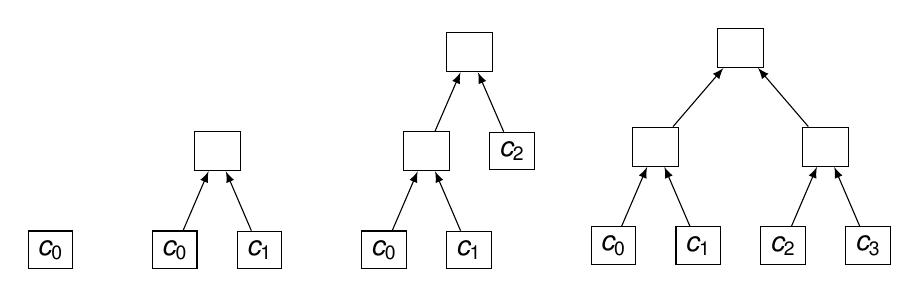
\begin{tikzpicture}

\node[draw,rectangle] (chunk1) at (0, 0) {$c_0$};

%%

\node[draw,rectangle,right=1cm of chunk1] (chunk2) {$c_0$};
\node[draw,rectangle,right=0.5cm of chunk2] (chunk3) {$c_1$};
\node[draw,rectangle,above=1cm of chunk2] (parent1) at ($(chunk2)!0.5!(chunk3)$) {\phantom{$p_0$}};
\draw[-latex] (chunk2) -- (parent1);
\draw[-latex] (chunk3) -- (parent1);

%%

\node[draw,rectangle,right=1cm of chunk3] (chunk2) {$c_0$};
\node[draw,rectangle,right=0.5cm of chunk2] (chunk3) {$c_1$};
\node[draw,rectangle,above=1cm of chunk2] (parent1) at ($(chunk2)!0.5!(chunk3)$) {\phantom{$p_0$}};
\node[draw,rectangle,right=0.5cm of parent1] (chunk4) {$c_2$};
\node[draw,rectangle,above=1cm of chunk4] (parent2) at ($(parent1)!0.5!(chunk4)$) {\phantom{$p_0$}};
\draw[-latex] (chunk2) -- (parent1);
\draw[-latex] (chunk3) -- (parent1);
\draw[-latex] (parent1) -- (parent2);
\draw[-latex] (chunk4) -- (parent2);

%%

\node[draw,rectangle,below right=1cm of chunk4] (chunk2) {$c_0$};
\node[draw,rectangle,right=0.5cm of chunk2] (chunk3) {$c_1$};
\node[draw,rectangle,above=1cm of chunk2] (parent1) at ($(chunk2)!0.5!(chunk3)$) {\phantom{$p_0$}};
\node[draw,rectangle,right=0.5cm of chunk3] (chunk4) {$c_2$};
\node[draw,rectangle,right=0.5cm of chunk4] (chunk5) {$c_3$};
\node[draw,rectangle,above=1cm of chunk4] (parent2) at ($(chunk4)!0.5!(chunk5)$) {\phantom{$p_0$}};
\node[draw,rectangle,above=1cm of parent2] (parent3) at ($(parent1)!0.5!(parent2)$) {\phantom{$p_0$}};
\draw[-latex] (chunk2) -- (parent1);
\draw[-latex] (chunk3) -- (parent1);
\draw[-latex] (chunk4) -- (parent2);
\draw[-latex] (chunk5) -- (parent2);
\draw[-latex] (parent1) -- (parent3);
\draw[-latex] (parent2) -- (parent3);

\end{tikzpicture}
\caption{Example tree structures, from 1 to 4 chunks.}
\label{fig:fourchunks}
\end{figure}

The compression function is used to derive a chaining value from each chunk and
parent node. The chaining value of the root node, encoded as 32 bytes in
little-endian order, is the default-length BLAKE3 hash of the input. BLAKE3
supports input of any byte length $0 \leq \ell < 2^{64}$.

\subsection{Compression Function}\label{sec:compression}

The compression function takes an 8-word chaining value and a 16-word message
block, and it returns a new 16-word value. A word is 32 bits. The inputs to
the compression function are:

\begin{itemize}
    \item The input chaining value, $h_{0} \ldots h_{7}$.
    \item The message block, $m_{0} \ldots m_{15}$.
    \item A 64-bit offset, $t=t_{0},t_{1}$, with $t_{0}$ the lower order word
        and $t_{1}$ the higher order word.
    \item The number of input bytes in the block, $b$.
    \item A set of domain separation bit flags, $d$.
\end{itemize}

The compression function initializes its 16-word internal state $v_{0} \ldots
v_{15}$ as follows: 

\begin{equation*}
\begin{pmatrix}
v_{0} & v_{1} & v_{2} & v_{3} \\
v_{4} & v_{5} & v_{6} & v_{7} \\
v_{8} & v_{9} & v_{10} & v_{11} \\
v_{12} & v_{13} & v_{14} & v_{15} \\
\end{pmatrix}
\leftarrow
\begin{pmatrix}
h_{0} & h_{1} & h_{2} & h_{3} \\
h_{4} & h_{5} & h_{6} & h_{7} \\
\IV_{0} & \IV_{1} & \IV_{2} & \IV_{3} \\
t_{0} & t_{1} & b & d 
\end{pmatrix}
\end{equation*}

The $\IV_{0} \ldots \IV_{7}$ constants are the same as in
BLAKE2s, and they are reproduced in Appendix~\ref{sec:ivconstants}.

The compression function applies a 7-round keyed permutation $v' = E(m, v)$ to
the state $v_0, \dots, v_{15}$, keyed by the message $m_0, \dots, m_{15}$. The
keyed permutation here is identical to the one underlying BLAKE2s, and is
reproduced in Appendix~\ref{sec:roundfn}.

The output of the compression function $h_{0}' \ldots h_{15}'$ is
defined as:
\begin{align*}
h_{0}'  \ & \leftarrow \ v'_{0} \oplus  v'_{8} &
h_{8}'  \ & \leftarrow \ v'_{8} \oplus  h_{0} \\
h_{1}'  \ & \leftarrow \ v'_{1} \oplus  v'_{9} &
h_{9}'  \ & \leftarrow \ v'_{9} \oplus  h_{1} \\
h_{2}'  \ & \leftarrow \ v'_{2} \oplus  v'_{10} &
h_{10}' \ & \leftarrow \ v'_{10} \oplus  h_{2} \\
h_{3}'  \ & \leftarrow \ v'_{3} \oplus  v'_{11} &
h_{11}' \ & \leftarrow \ v'_{11} \oplus  h_{3} \\
h_{4}'  \ & \leftarrow \ v'_{4} \oplus  v'_{12} &
h_{12}' \ & \leftarrow \ v'_{12} \oplus  h_{4} \\
h_{5}'  \ & \leftarrow \ v'_{5} \oplus  v'_{13} &
h_{13}' \ & \leftarrow \ v'_{13} \oplus  h_{5} \\
h_{6}'  \ & \leftarrow \ v'_{6} \oplus  v'_{14} &
h_{14}' \ & \leftarrow \ v'_{14} \oplus  h_{6} \\
h_{7}'  \ & \leftarrow \ v'_{7} \oplus  v'_{15} &
h_{15}' \ & \leftarrow \ v'_{15} \oplus  h_{7}\,.
\end{align*}
If we define $v_l$ (resp. $v'_l$) and $v_h$ (resp. $v'_h$) as the first and last 8-words of the input (resp. output) of $E(m, v)$ as elements of $\mathbb{F}_2^{256}$, the compression function may be represented as 
\[
  \begin{pmatrix}
    1 & 1 \\
    0 & 1
  \end{pmatrix}\cdot%
  \begin{pmatrix}
  v'_l \\ v'_h
  \end{pmatrix} + 
  \begin{pmatrix}
   0 \\ v_l
  \end{pmatrix}\,.
\]
A common variant of the compression function, used internally to produce 256-bit chaining values, simply truncates the output to its first 256 bits. We defer to analysis of the compression function to \S\ref{sec:security}.

%\subsubsection{Flags}
The compression function input $d$ is a bitfield, with each individual flag consisting of a power of 2 value. The value of $d$ is the sum of all the flags defined for a given
compression. Their names and values are given in Table~\ref{tab:flags}.
\begin{table}
  \centering
  \caption{Admissible values for input $d$ in the BLAKE3 compression function.}%
  \label{tab:flags}
  \begin{tabular}{cc}
    \toprule
    Flag name             & Value \\ \midrule
    \texttt{CHUNK\_START} & $2^0$ \\
    \texttt{CHUNK\_END}   & $2^1$ \\
    \texttt{PARENT}       & $2^2$ \\
    \texttt{ROOT}         & $2^3$ \\
    \texttt{KEYED\_HASH}  & $2^4$ \\
    \texttt{DERIVE\_KEY}  & $2^5$ \\
    \bottomrule
  \end{tabular}
\end{table}

\subsection{Modes}\label{sec:modes}

BLAKE3 defines three domain-separated modes: \texttt{hash},
\texttt{keyed\_hash}, and \texttt{derive\_key}. The modes differ from each
other in their key words $k_{0} \ldots k_{7}$ and in the additional flags they
set for every call to the compression function:

\begin{itemize}
  \item In the \texttt{hash} mode, $k_{0} \ldots k_{7}$ are the constants $\IV_0 \ldots \IV_7$, and no additional flags are set. 
  \item In the \texttt{keyed\_hash} mode, $k_{0} \ldots k_{7}$ are parsed in little-endian order from the 32-byte key given by the caller, and the \texttt{KEYED\_HASH} flag is set for every compression.
  \item  In the \texttt{derive\_key} mode, the key is again given by the caller, and the \texttt{DERIVE\_KEY} flag is set for every compression.
\end{itemize}

\subsection{Chunk Chaining Values}\label{sec:chunk}

Processing a chunk is structurally similar to the sequential hashing mode of BLAKE2. Each chunk of up to 2048 bytes is split into blocks of up to 64 bytes.
The last block of the last chunk may be shorter, but not empty, unless the
entire input is empty. The last block, if necessary, is padded with zeros to be 64
bytes. 

Each block is parsed in little-endian order into message words $m_{0}
\ldots m_{15}$ and compressed. The input chaining value $h_{0} \ldots h_{7}$
for the first block of each chunk is comprised of the key words $k_{0} \ldots k_{7}$. The
input chaining value for subsequent blocks in each chunk is the output of the truncated
compression function for the previous block. 

The remaining compression function parameters are handled as follows (see also Figure~\ref{fig:chunk} for an example):
\begin{itemize}
\item The offset $t$ for each block is
the starting byte index of its chunk, i.e., $0$ for all blocks in the first chunk, $2048$
for all blocks in the second chunk, and so on. 
\item The block length $b$ is the
number of input bytes in each block, i.e., $64$ for all blocks except the last block of
the last chunk, which may be short. 
\item The first block of each chunk sets the
\texttt{CHUNK\_START} flag (cf. Table~\ref{tab:flags}), and the last block of each chunk sets the
\texttt{CHUNK\_END} flag. If a chunk contains only one block, that block sets
both \texttt{CHUNK\_START} and \texttt{CHUNK\_END}. If a chunk is the root of
its tree, the last block of that chunk also sets the \texttt{ROOT} flag.
\end{itemize}

The output of the truncated compression function for the last block in a chunk
is the chaining value of that chunk.

\begin{figure}
\centering
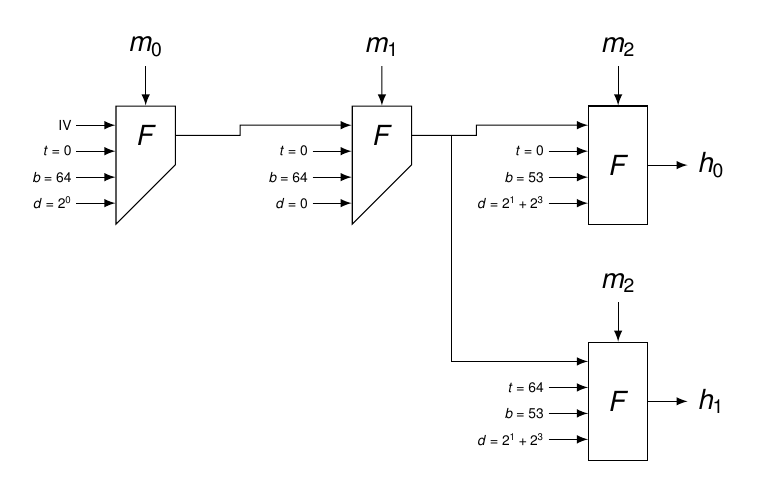
\begin{tikzpicture}[
comp/.style={draw, trapezium, trapezium left angle=0, trapezium right angle=45, shape border rotate=270, minimum height=0.5cm, minimum width=1.5cm, trapezium stretches=false,anchor=north},
fullcomp/.style={draw, rectangle, minimum height=1.5cm, minimum width=0.75cm, trapezium stretches=false,anchor=north},
]

\begin{scope}[xshift=0cm]
\node[comp] (f0) {$F$};
\node[above=0.5cm of f0] (m0) {$m_0$};
\coordinate (tmp) at ($(f0.north west) + (-0.5cm, -0.25cm)$);
\node[below = 0.00cm of tmp,scale=0.50,anchor=east] (iv) {$\mathrm{IV}$};
\node[below = 0.33cm of tmp,scale=0.50,anchor=east] (t0) {$t=0$};
\node[below = 0.66cm of tmp,scale=0.50,anchor=east] (b0) {$b=64$};
\node[below = 0.99cm of tmp,scale=0.50,anchor=east] (d0) {$d=2^0$};

\draw[-latex] (m0) -- (f0);
\draw[-latex] (iv) -- (iv -| f0.west);
\draw[-latex] (t0) -- (t0 -| f0.west);
\draw[-latex] (b0) -- (b0 -| f0.west);
\draw[-latex] (d0) -- (d0 -| f0.west);
\end{scope}

\begin{scope}[xshift=3cm]
\node[comp] (f1) {$F$};
\node[above=0.5cm of f1] (m1) {$m_1$};
\coordinate (tmp) at ($(f1.north west) + (-0.5cm, -0.25cm)$);

\node[below = 0.33cm of tmp,scale=0.5,anchor=east] (t1) {$t=0$};
\node[below = 0.66cm of tmp,scale=0.5,anchor=east] (b1) {$b=64$};
\node[below = 0.99cm of tmp,scale=0.5,anchor=east] (d1) {$d=0$};

\draw[-latex] (m1) -- (f1);
\draw[-latex] (t1) -- (t1 -| f1.west);
\draw[-latex] (b1) -- (b1 -| f1.west);
\draw[-latex] (d1) -- (d1 -| f1.west);
\end{scope}

\begin{scope}[xshift=6cm]
\node[fullcomp] (f2) {$F$};
\node[above=0.5cm of f2] (m2) {$m_2$};
\coordinate (tmp) at ($(f2.north west) + (-0.5cm, -0.25cm)$);

\node[below = 0.33cm of tmp,scale=0.5,anchor=east] (t2) {$t=0$};
\node[below = 0.66cm of tmp,scale=0.5,anchor=east] (b2) {$b=53$};
\node[below = 0.99cm of tmp,scale=0.5,anchor=east] (d2) {$d=2^1+2^3$};

\draw[-latex] (m2) -- (f2);
\draw[-latex] (t2) -- (t2 -| f2.west);
\draw[-latex] (b2) -- (b2 -| f2.west);
\draw[-latex] (d2) -- (d2 -| f2.west);
\end{scope}

\begin{scope}[xshift=6cm,yshift=-3cm]
\node[fullcomp] (f3) {$F$};
\node[above=0.5cm of f3] (m3) {$m_2$};
\coordinate (tmp) at ($(f3.north west) + (-0.5cm, -0.25cm)$);

\node[below = 0.33cm of tmp,scale=0.5,anchor=east] (t3) {$t=64$};
\node[below = 0.66cm of tmp,scale=0.5,anchor=east] (b3) {$b=53$};
\node[below = 0.99cm of tmp,scale=0.5,anchor=east] (d3) {$d=2^1+2^3$};

\draw[-latex] (m3) -- (f3);
\draw[-latex] (t3) -- (t3 -| f3.west);
\draw[-latex] (b3) -- (b3 -| f3.west);
\draw[-latex] (d3) -- (d3 -| f3.west);
\end{scope}

\coordinate (tmp) at (f1.west |- iv);
\coordinate (tmp2) at ($(f0)!0.40!(f1)$);
\draw[-latex] (f0) -- (f0 -| tmp2) -- (tmp2 |- tmp) -- (tmp);
\coordinate (tmp) at (f2.west |- iv);
\coordinate (tmp2) at ($(f1)!0.40!(f2)$);
\draw[-latex] (f1) -- (f1 -| tmp2) -- (tmp2 |- tmp) -- (tmp);

\coordinate (tmp) at ($(f3.north west) + (-0cm, -0.25cm)$);
\coordinate (tmp2) at ($(f1.east) + (0.5cm, 0)$);
\draw[-latex] (f1.east) -- (tmp2) -- (tmp2 |- tmp) -- (tmp);

\node[right=0.5cm of f2] (out) {$h_0$};
\draw[-latex] (f2) -- (out);
\node[right=0.5cm of f3] (out) {$h_1$};
\draw[-latex] (f3) -- (out);

\end{tikzpicture}
\caption{Example of compression function inputs when hashing a 181-byte input $(m_0, m_1, m_2)$ into a 128-byte output $(h_0, h_1)$. Trapezia indicate that the compression function output is truncated to 256 bits.}\label{fig:chunk}
\end{figure}

\subsection{Parent Node Chaining Values}\label{sec:parent}

Each parent node has exactly two children, each either a chunk or another
parent node. The chaining value of each parent node is given by a single call
to the compression function. The input chaining value $h_{0} \ldots h_{7}$ is
the key words $k_{0} \ldots k_{7}$. The message words $m_{0} \ldots m_{7}$ are
the chaining value of the left child, and the message words $m_{8} \ldots
m_{15}$ are the chaining value of the right child. The offset $t$ for parent
nodes is always 0. The number of bytes $b$ for parent nodes is always 64.
Parent nodes set the \texttt{PARENT} flag. If a parent node is the root of the
tree, it also sets the \texttt{ROOT} flag. The output of the truncated
compression function is the chaining value of the parent node.

\subsection{Extendable Output}\label{sec:extendable}

BLAKE3 can produce outputs of any byte length up to $2^{64}$ bytes. 
This is done by repeating the root compression---that is, the very last 
call to the compression function, which sets the \texttt{ROOT} flag---with 
incrementing values of the offset $t$. The results of these repeated root 
compressions are then concatenated to form the output.

When building the output, BLAKE3 uses the full output of the
compression function (cf. \S\ref{sec:compression}). Each 16-word output is
encoded as 64 bytes in little-endian order.

Observe that for the first output, the root compression always uses offset $t
= 0$. That is either because it is the last block of the only chunk, which has
a chunk offset of $0$, or because it is a parent node. Then as long as more 
bytes are needed, $t$ is incremented by 64, and the root compression is 
repeated on the same inputs. If the target output length is not a multiple of 64, 
the final compression output is truncated.

Because the repeated root compressions differ only in the value of $t$, the
implementation can execute any number of them in parallel. The caller can also
adjust $t$ to seek to any point in the output stream.

Note that in contrast to BLAKE2 and BLAKE2X, BLAKE3 does not domain separate
outputs of different lengths. Shorter outputs are prefixes of longer ones.

\section{Performance}\label{sec:performance}

\begin{figure}[h]
%% Creator: Matplotlib, PGF backend
%%
%% To include the figure in your LaTeX document, write
%%   \input{<filename>.pgf}
%%
%% Make sure the required packages are loaded in your preamble
%%   \usepackage{pgf}
%%
%% Figures using additional raster images can only be included by \input if
%% they are in the same directory as the main LaTeX file. For loading figures
%% from other directories you can use the `import` package
%%   \usepackage{import}
%% and then include the figures with
%%   \import{<path to file>}{<filename>.pgf}
%%
%% Matplotlib used the following preamble
%%   \usepackage{fontspec}
%%   \setmainfont{DejaVuSerif.ttf}[Path=/usr/lib/python3.8/site-packages/matplotlib/mpl-data/fonts/ttf/]
%%   \setsansfont{DejaVuSans.ttf}[Path=/usr/lib/python3.8/site-packages/matplotlib/mpl-data/fonts/ttf/]
%%   \setmonofont{DejaVuSansMono.ttf}[Path=/usr/lib/python3.8/site-packages/matplotlib/mpl-data/fonts/ttf/]
%%
\begingroup%
\makeatletter%
\begin{pgfpicture}%
\pgfpathrectangle{\pgfpointorigin}{\pgfqpoint{6.084224in}{4.615557in}}%
\pgfusepath{use as bounding box, clip}%
\begin{pgfscope}%
\pgfsetbuttcap%
\pgfsetmiterjoin%
\definecolor{currentfill}{rgb}{1.000000,1.000000,1.000000}%
\pgfsetfillcolor{currentfill}%
\pgfsetlinewidth{0.000000pt}%
\definecolor{currentstroke}{rgb}{1.000000,1.000000,1.000000}%
\pgfsetstrokecolor{currentstroke}%
\pgfsetdash{}{0pt}%
\pgfpathmoveto{\pgfqpoint{0.000000in}{0.000000in}}%
\pgfpathlineto{\pgfqpoint{6.084224in}{0.000000in}}%
\pgfpathlineto{\pgfqpoint{6.084224in}{4.615557in}}%
\pgfpathlineto{\pgfqpoint{0.000000in}{4.615557in}}%
\pgfpathclose%
\pgfusepath{fill}%
\end{pgfscope}%
\begin{pgfscope}%
\pgfsetbuttcap%
\pgfsetmiterjoin%
\definecolor{currentfill}{rgb}{0.917647,0.917647,0.949020}%
\pgfsetfillcolor{currentfill}%
\pgfsetlinewidth{0.000000pt}%
\definecolor{currentstroke}{rgb}{0.000000,0.000000,0.000000}%
\pgfsetstrokecolor{currentstroke}%
\pgfsetstrokeopacity{0.000000}%
\pgfsetdash{}{0pt}%
\pgfpathmoveto{\pgfqpoint{1.024224in}{0.819557in}}%
\pgfpathlineto{\pgfqpoint{5.984224in}{0.819557in}}%
\pgfpathlineto{\pgfqpoint{5.984224in}{4.515557in}}%
\pgfpathlineto{\pgfqpoint{1.024224in}{4.515557in}}%
\pgfpathclose%
\pgfusepath{fill}%
\end{pgfscope}%
\begin{pgfscope}%
\pgfpathrectangle{\pgfqpoint{1.024224in}{0.819557in}}{\pgfqpoint{4.960000in}{3.696000in}}%
\pgfusepath{clip}%
\pgfsetroundcap%
\pgfsetroundjoin%
\pgfsetlinewidth{1.003750pt}%
\definecolor{currentstroke}{rgb}{1.000000,1.000000,1.000000}%
\pgfsetstrokecolor{currentstroke}%
\pgfsetdash{}{0pt}%
\pgfpathmoveto{\pgfqpoint{1.249678in}{0.819557in}}%
\pgfpathlineto{\pgfqpoint{1.249678in}{4.515557in}}%
\pgfusepath{stroke}%
\end{pgfscope}%
\begin{pgfscope}%
\definecolor{textcolor}{rgb}{0.150000,0.150000,0.150000}%
\pgfsetstrokecolor{textcolor}%
\pgfsetfillcolor{textcolor}%
\pgftext[x=1.207530in,y=0.687613in,left,base,rotate=270.000000]{\color{textcolor}\sffamily\fontsize{11.000000}{13.200000}\selectfont 64}%
\end{pgfscope}%
\begin{pgfscope}%
\pgfpathrectangle{\pgfqpoint{1.024224in}{0.819557in}}{\pgfqpoint{4.960000in}{3.696000in}}%
\pgfusepath{clip}%
\pgfsetroundcap%
\pgfsetroundjoin%
\pgfsetlinewidth{1.003750pt}%
\definecolor{currentstroke}{rgb}{1.000000,1.000000,1.000000}%
\pgfsetstrokecolor{currentstroke}%
\pgfsetdash{}{0pt}%
\pgfpathmoveto{\pgfqpoint{1.500183in}{0.819557in}}%
\pgfpathlineto{\pgfqpoint{1.500183in}{4.515557in}}%
\pgfusepath{stroke}%
\end{pgfscope}%
\begin{pgfscope}%
\definecolor{textcolor}{rgb}{0.150000,0.150000,0.150000}%
\pgfsetstrokecolor{textcolor}%
\pgfsetfillcolor{textcolor}%
\pgftext[x=1.458035in,y=0.687613in,left,base,rotate=270.000000]{\color{textcolor}\sffamily\fontsize{11.000000}{13.200000}\selectfont 128}%
\end{pgfscope}%
\begin{pgfscope}%
\pgfpathrectangle{\pgfqpoint{1.024224in}{0.819557in}}{\pgfqpoint{4.960000in}{3.696000in}}%
\pgfusepath{clip}%
\pgfsetroundcap%
\pgfsetroundjoin%
\pgfsetlinewidth{1.003750pt}%
\definecolor{currentstroke}{rgb}{1.000000,1.000000,1.000000}%
\pgfsetstrokecolor{currentstroke}%
\pgfsetdash{}{0pt}%
\pgfpathmoveto{\pgfqpoint{1.750689in}{0.819557in}}%
\pgfpathlineto{\pgfqpoint{1.750689in}{4.515557in}}%
\pgfusepath{stroke}%
\end{pgfscope}%
\begin{pgfscope}%
\definecolor{textcolor}{rgb}{0.150000,0.150000,0.150000}%
\pgfsetstrokecolor{textcolor}%
\pgfsetfillcolor{textcolor}%
\pgftext[x=1.708540in,y=0.687613in,left,base,rotate=270.000000]{\color{textcolor}\sffamily\fontsize{11.000000}{13.200000}\selectfont 256}%
\end{pgfscope}%
\begin{pgfscope}%
\pgfpathrectangle{\pgfqpoint{1.024224in}{0.819557in}}{\pgfqpoint{4.960000in}{3.696000in}}%
\pgfusepath{clip}%
\pgfsetroundcap%
\pgfsetroundjoin%
\pgfsetlinewidth{1.003750pt}%
\definecolor{currentstroke}{rgb}{1.000000,1.000000,1.000000}%
\pgfsetstrokecolor{currentstroke}%
\pgfsetdash{}{0pt}%
\pgfpathmoveto{\pgfqpoint{2.001194in}{0.819557in}}%
\pgfpathlineto{\pgfqpoint{2.001194in}{4.515557in}}%
\pgfusepath{stroke}%
\end{pgfscope}%
\begin{pgfscope}%
\definecolor{textcolor}{rgb}{0.150000,0.150000,0.150000}%
\pgfsetstrokecolor{textcolor}%
\pgfsetfillcolor{textcolor}%
\pgftext[x=1.959045in,y=0.687613in,left,base,rotate=270.000000]{\color{textcolor}\sffamily\fontsize{11.000000}{13.200000}\selectfont 512}%
\end{pgfscope}%
\begin{pgfscope}%
\pgfpathrectangle{\pgfqpoint{1.024224in}{0.819557in}}{\pgfqpoint{4.960000in}{3.696000in}}%
\pgfusepath{clip}%
\pgfsetroundcap%
\pgfsetroundjoin%
\pgfsetlinewidth{1.003750pt}%
\definecolor{currentstroke}{rgb}{1.000000,1.000000,1.000000}%
\pgfsetstrokecolor{currentstroke}%
\pgfsetdash{}{0pt}%
\pgfpathmoveto{\pgfqpoint{2.251699in}{0.819557in}}%
\pgfpathlineto{\pgfqpoint{2.251699in}{4.515557in}}%
\pgfusepath{stroke}%
\end{pgfscope}%
\begin{pgfscope}%
\definecolor{textcolor}{rgb}{0.150000,0.150000,0.150000}%
\pgfsetstrokecolor{textcolor}%
\pgfsetfillcolor{textcolor}%
\pgftext[x=2.209550in,y=0.687613in,left,base,rotate=270.000000]{\color{textcolor}\sffamily\fontsize{11.000000}{13.200000}\selectfont 1 KiB}%
\end{pgfscope}%
\begin{pgfscope}%
\pgfpathrectangle{\pgfqpoint{1.024224in}{0.819557in}}{\pgfqpoint{4.960000in}{3.696000in}}%
\pgfusepath{clip}%
\pgfsetroundcap%
\pgfsetroundjoin%
\pgfsetlinewidth{1.003750pt}%
\definecolor{currentstroke}{rgb}{1.000000,1.000000,1.000000}%
\pgfsetstrokecolor{currentstroke}%
\pgfsetdash{}{0pt}%
\pgfpathmoveto{\pgfqpoint{2.502204in}{0.819557in}}%
\pgfpathlineto{\pgfqpoint{2.502204in}{4.515557in}}%
\pgfusepath{stroke}%
\end{pgfscope}%
\begin{pgfscope}%
\definecolor{textcolor}{rgb}{0.150000,0.150000,0.150000}%
\pgfsetstrokecolor{textcolor}%
\pgfsetfillcolor{textcolor}%
\pgftext[x=2.460055in,y=0.687613in,left,base,rotate=270.000000]{\color{textcolor}\sffamily\fontsize{11.000000}{13.200000}\selectfont 2 KiB}%
\end{pgfscope}%
\begin{pgfscope}%
\pgfpathrectangle{\pgfqpoint{1.024224in}{0.819557in}}{\pgfqpoint{4.960000in}{3.696000in}}%
\pgfusepath{clip}%
\pgfsetroundcap%
\pgfsetroundjoin%
\pgfsetlinewidth{1.003750pt}%
\definecolor{currentstroke}{rgb}{1.000000,1.000000,1.000000}%
\pgfsetstrokecolor{currentstroke}%
\pgfsetdash{}{0pt}%
\pgfpathmoveto{\pgfqpoint{2.752709in}{0.819557in}}%
\pgfpathlineto{\pgfqpoint{2.752709in}{4.515557in}}%
\pgfusepath{stroke}%
\end{pgfscope}%
\begin{pgfscope}%
\definecolor{textcolor}{rgb}{0.150000,0.150000,0.150000}%
\pgfsetstrokecolor{textcolor}%
\pgfsetfillcolor{textcolor}%
\pgftext[x=2.710560in,y=0.687613in,left,base,rotate=270.000000]{\color{textcolor}\sffamily\fontsize{11.000000}{13.200000}\selectfont 4 KiB}%
\end{pgfscope}%
\begin{pgfscope}%
\pgfpathrectangle{\pgfqpoint{1.024224in}{0.819557in}}{\pgfqpoint{4.960000in}{3.696000in}}%
\pgfusepath{clip}%
\pgfsetroundcap%
\pgfsetroundjoin%
\pgfsetlinewidth{1.003750pt}%
\definecolor{currentstroke}{rgb}{1.000000,1.000000,1.000000}%
\pgfsetstrokecolor{currentstroke}%
\pgfsetdash{}{0pt}%
\pgfpathmoveto{\pgfqpoint{3.003214in}{0.819557in}}%
\pgfpathlineto{\pgfqpoint{3.003214in}{4.515557in}}%
\pgfusepath{stroke}%
\end{pgfscope}%
\begin{pgfscope}%
\definecolor{textcolor}{rgb}{0.150000,0.150000,0.150000}%
\pgfsetstrokecolor{textcolor}%
\pgfsetfillcolor{textcolor}%
\pgftext[x=2.961065in,y=0.687613in,left,base,rotate=270.000000]{\color{textcolor}\sffamily\fontsize{11.000000}{13.200000}\selectfont 8 KiB}%
\end{pgfscope}%
\begin{pgfscope}%
\pgfpathrectangle{\pgfqpoint{1.024224in}{0.819557in}}{\pgfqpoint{4.960000in}{3.696000in}}%
\pgfusepath{clip}%
\pgfsetroundcap%
\pgfsetroundjoin%
\pgfsetlinewidth{1.003750pt}%
\definecolor{currentstroke}{rgb}{1.000000,1.000000,1.000000}%
\pgfsetstrokecolor{currentstroke}%
\pgfsetdash{}{0pt}%
\pgfpathmoveto{\pgfqpoint{3.253719in}{0.819557in}}%
\pgfpathlineto{\pgfqpoint{3.253719in}{4.515557in}}%
\pgfusepath{stroke}%
\end{pgfscope}%
\begin{pgfscope}%
\definecolor{textcolor}{rgb}{0.150000,0.150000,0.150000}%
\pgfsetstrokecolor{textcolor}%
\pgfsetfillcolor{textcolor}%
\pgftext[x=3.211571in,y=0.687613in,left,base,rotate=270.000000]{\color{textcolor}\sffamily\fontsize{11.000000}{13.200000}\selectfont 16 KiB}%
\end{pgfscope}%
\begin{pgfscope}%
\pgfpathrectangle{\pgfqpoint{1.024224in}{0.819557in}}{\pgfqpoint{4.960000in}{3.696000in}}%
\pgfusepath{clip}%
\pgfsetroundcap%
\pgfsetroundjoin%
\pgfsetlinewidth{1.003750pt}%
\definecolor{currentstroke}{rgb}{1.000000,1.000000,1.000000}%
\pgfsetstrokecolor{currentstroke}%
\pgfsetdash{}{0pt}%
\pgfpathmoveto{\pgfqpoint{3.504224in}{0.819557in}}%
\pgfpathlineto{\pgfqpoint{3.504224in}{4.515557in}}%
\pgfusepath{stroke}%
\end{pgfscope}%
\begin{pgfscope}%
\definecolor{textcolor}{rgb}{0.150000,0.150000,0.150000}%
\pgfsetstrokecolor{textcolor}%
\pgfsetfillcolor{textcolor}%
\pgftext[x=3.462076in,y=0.687613in,left,base,rotate=270.000000]{\color{textcolor}\sffamily\fontsize{11.000000}{13.200000}\selectfont 32 KiB}%
\end{pgfscope}%
\begin{pgfscope}%
\pgfpathrectangle{\pgfqpoint{1.024224in}{0.819557in}}{\pgfqpoint{4.960000in}{3.696000in}}%
\pgfusepath{clip}%
\pgfsetroundcap%
\pgfsetroundjoin%
\pgfsetlinewidth{1.003750pt}%
\definecolor{currentstroke}{rgb}{1.000000,1.000000,1.000000}%
\pgfsetstrokecolor{currentstroke}%
\pgfsetdash{}{0pt}%
\pgfpathmoveto{\pgfqpoint{3.754729in}{0.819557in}}%
\pgfpathlineto{\pgfqpoint{3.754729in}{4.515557in}}%
\pgfusepath{stroke}%
\end{pgfscope}%
\begin{pgfscope}%
\definecolor{textcolor}{rgb}{0.150000,0.150000,0.150000}%
\pgfsetstrokecolor{textcolor}%
\pgfsetfillcolor{textcolor}%
\pgftext[x=3.712581in,y=0.687613in,left,base,rotate=270.000000]{\color{textcolor}\sffamily\fontsize{11.000000}{13.200000}\selectfont 64 KiB}%
\end{pgfscope}%
\begin{pgfscope}%
\pgfpathrectangle{\pgfqpoint{1.024224in}{0.819557in}}{\pgfqpoint{4.960000in}{3.696000in}}%
\pgfusepath{clip}%
\pgfsetroundcap%
\pgfsetroundjoin%
\pgfsetlinewidth{1.003750pt}%
\definecolor{currentstroke}{rgb}{1.000000,1.000000,1.000000}%
\pgfsetstrokecolor{currentstroke}%
\pgfsetdash{}{0pt}%
\pgfpathmoveto{\pgfqpoint{4.005234in}{0.819557in}}%
\pgfpathlineto{\pgfqpoint{4.005234in}{4.515557in}}%
\pgfusepath{stroke}%
\end{pgfscope}%
\begin{pgfscope}%
\definecolor{textcolor}{rgb}{0.150000,0.150000,0.150000}%
\pgfsetstrokecolor{textcolor}%
\pgfsetfillcolor{textcolor}%
\pgftext[x=3.963086in,y=0.687613in,left,base,rotate=270.000000]{\color{textcolor}\sffamily\fontsize{11.000000}{13.200000}\selectfont 128 KiB}%
\end{pgfscope}%
\begin{pgfscope}%
\pgfpathrectangle{\pgfqpoint{1.024224in}{0.819557in}}{\pgfqpoint{4.960000in}{3.696000in}}%
\pgfusepath{clip}%
\pgfsetroundcap%
\pgfsetroundjoin%
\pgfsetlinewidth{1.003750pt}%
\definecolor{currentstroke}{rgb}{1.000000,1.000000,1.000000}%
\pgfsetstrokecolor{currentstroke}%
\pgfsetdash{}{0pt}%
\pgfpathmoveto{\pgfqpoint{4.255739in}{0.819557in}}%
\pgfpathlineto{\pgfqpoint{4.255739in}{4.515557in}}%
\pgfusepath{stroke}%
\end{pgfscope}%
\begin{pgfscope}%
\definecolor{textcolor}{rgb}{0.150000,0.150000,0.150000}%
\pgfsetstrokecolor{textcolor}%
\pgfsetfillcolor{textcolor}%
\pgftext[x=4.213591in,y=0.687613in,left,base,rotate=270.000000]{\color{textcolor}\sffamily\fontsize{11.000000}{13.200000}\selectfont 256 KiB}%
\end{pgfscope}%
\begin{pgfscope}%
\pgfpathrectangle{\pgfqpoint{1.024224in}{0.819557in}}{\pgfqpoint{4.960000in}{3.696000in}}%
\pgfusepath{clip}%
\pgfsetroundcap%
\pgfsetroundjoin%
\pgfsetlinewidth{1.003750pt}%
\definecolor{currentstroke}{rgb}{1.000000,1.000000,1.000000}%
\pgfsetstrokecolor{currentstroke}%
\pgfsetdash{}{0pt}%
\pgfpathmoveto{\pgfqpoint{4.506244in}{0.819557in}}%
\pgfpathlineto{\pgfqpoint{4.506244in}{4.515557in}}%
\pgfusepath{stroke}%
\end{pgfscope}%
\begin{pgfscope}%
\definecolor{textcolor}{rgb}{0.150000,0.150000,0.150000}%
\pgfsetstrokecolor{textcolor}%
\pgfsetfillcolor{textcolor}%
\pgftext[x=4.464096in,y=0.687613in,left,base,rotate=270.000000]{\color{textcolor}\sffamily\fontsize{11.000000}{13.200000}\selectfont 512 KiB}%
\end{pgfscope}%
\begin{pgfscope}%
\pgfpathrectangle{\pgfqpoint{1.024224in}{0.819557in}}{\pgfqpoint{4.960000in}{3.696000in}}%
\pgfusepath{clip}%
\pgfsetroundcap%
\pgfsetroundjoin%
\pgfsetlinewidth{1.003750pt}%
\definecolor{currentstroke}{rgb}{1.000000,1.000000,1.000000}%
\pgfsetstrokecolor{currentstroke}%
\pgfsetdash{}{0pt}%
\pgfpathmoveto{\pgfqpoint{4.756749in}{0.819557in}}%
\pgfpathlineto{\pgfqpoint{4.756749in}{4.515557in}}%
\pgfusepath{stroke}%
\end{pgfscope}%
\begin{pgfscope}%
\definecolor{textcolor}{rgb}{0.150000,0.150000,0.150000}%
\pgfsetstrokecolor{textcolor}%
\pgfsetfillcolor{textcolor}%
\pgftext[x=4.714601in,y=0.687613in,left,base,rotate=270.000000]{\color{textcolor}\sffamily\fontsize{11.000000}{13.200000}\selectfont 1 MiB}%
\end{pgfscope}%
\begin{pgfscope}%
\pgfpathrectangle{\pgfqpoint{1.024224in}{0.819557in}}{\pgfqpoint{4.960000in}{3.696000in}}%
\pgfusepath{clip}%
\pgfsetroundcap%
\pgfsetroundjoin%
\pgfsetlinewidth{1.003750pt}%
\definecolor{currentstroke}{rgb}{1.000000,1.000000,1.000000}%
\pgfsetstrokecolor{currentstroke}%
\pgfsetdash{}{0pt}%
\pgfpathmoveto{\pgfqpoint{5.007254in}{0.819557in}}%
\pgfpathlineto{\pgfqpoint{5.007254in}{4.515557in}}%
\pgfusepath{stroke}%
\end{pgfscope}%
\begin{pgfscope}%
\definecolor{textcolor}{rgb}{0.150000,0.150000,0.150000}%
\pgfsetstrokecolor{textcolor}%
\pgfsetfillcolor{textcolor}%
\pgftext[x=4.965106in,y=0.687613in,left,base,rotate=270.000000]{\color{textcolor}\sffamily\fontsize{11.000000}{13.200000}\selectfont 2 MiB}%
\end{pgfscope}%
\begin{pgfscope}%
\pgfpathrectangle{\pgfqpoint{1.024224in}{0.819557in}}{\pgfqpoint{4.960000in}{3.696000in}}%
\pgfusepath{clip}%
\pgfsetroundcap%
\pgfsetroundjoin%
\pgfsetlinewidth{1.003750pt}%
\definecolor{currentstroke}{rgb}{1.000000,1.000000,1.000000}%
\pgfsetstrokecolor{currentstroke}%
\pgfsetdash{}{0pt}%
\pgfpathmoveto{\pgfqpoint{5.257759in}{0.819557in}}%
\pgfpathlineto{\pgfqpoint{5.257759in}{4.515557in}}%
\pgfusepath{stroke}%
\end{pgfscope}%
\begin{pgfscope}%
\definecolor{textcolor}{rgb}{0.150000,0.150000,0.150000}%
\pgfsetstrokecolor{textcolor}%
\pgfsetfillcolor{textcolor}%
\pgftext[x=5.215611in,y=0.687613in,left,base,rotate=270.000000]{\color{textcolor}\sffamily\fontsize{11.000000}{13.200000}\selectfont 4 MiB}%
\end{pgfscope}%
\begin{pgfscope}%
\pgfpathrectangle{\pgfqpoint{1.024224in}{0.819557in}}{\pgfqpoint{4.960000in}{3.696000in}}%
\pgfusepath{clip}%
\pgfsetroundcap%
\pgfsetroundjoin%
\pgfsetlinewidth{1.003750pt}%
\definecolor{currentstroke}{rgb}{1.000000,1.000000,1.000000}%
\pgfsetstrokecolor{currentstroke}%
\pgfsetdash{}{0pt}%
\pgfpathmoveto{\pgfqpoint{5.508264in}{0.819557in}}%
\pgfpathlineto{\pgfqpoint{5.508264in}{4.515557in}}%
\pgfusepath{stroke}%
\end{pgfscope}%
\begin{pgfscope}%
\definecolor{textcolor}{rgb}{0.150000,0.150000,0.150000}%
\pgfsetstrokecolor{textcolor}%
\pgfsetfillcolor{textcolor}%
\pgftext[x=5.466116in,y=0.687613in,left,base,rotate=270.000000]{\color{textcolor}\sffamily\fontsize{11.000000}{13.200000}\selectfont 8 MiB}%
\end{pgfscope}%
\begin{pgfscope}%
\pgfpathrectangle{\pgfqpoint{1.024224in}{0.819557in}}{\pgfqpoint{4.960000in}{3.696000in}}%
\pgfusepath{clip}%
\pgfsetroundcap%
\pgfsetroundjoin%
\pgfsetlinewidth{1.003750pt}%
\definecolor{currentstroke}{rgb}{1.000000,1.000000,1.000000}%
\pgfsetstrokecolor{currentstroke}%
\pgfsetdash{}{0pt}%
\pgfpathmoveto{\pgfqpoint{5.758769in}{0.819557in}}%
\pgfpathlineto{\pgfqpoint{5.758769in}{4.515557in}}%
\pgfusepath{stroke}%
\end{pgfscope}%
\begin{pgfscope}%
\definecolor{textcolor}{rgb}{0.150000,0.150000,0.150000}%
\pgfsetstrokecolor{textcolor}%
\pgfsetfillcolor{textcolor}%
\pgftext[x=5.716621in,y=0.687613in,left,base,rotate=270.000000]{\color{textcolor}\sffamily\fontsize{11.000000}{13.200000}\selectfont 16 MiB}%
\end{pgfscope}%
\begin{pgfscope}%
\pgfpathrectangle{\pgfqpoint{1.024224in}{0.819557in}}{\pgfqpoint{4.960000in}{3.696000in}}%
\pgfusepath{clip}%
\pgfsetroundcap%
\pgfsetroundjoin%
\pgfsetlinewidth{1.003750pt}%
\definecolor{currentstroke}{rgb}{1.000000,1.000000,1.000000}%
\pgfsetstrokecolor{currentstroke}%
\pgfsetdash{}{0pt}%
\pgfpathmoveto{\pgfqpoint{1.024224in}{0.819557in}}%
\pgfpathlineto{\pgfqpoint{5.984224in}{0.819557in}}%
\pgfusepath{stroke}%
\end{pgfscope}%
\begin{pgfscope}%
\definecolor{textcolor}{rgb}{0.150000,0.150000,0.150000}%
\pgfsetstrokecolor{textcolor}%
\pgfsetfillcolor{textcolor}%
\pgftext[x=0.795077in,y=0.761519in,left,base]{\color{textcolor}\sffamily\fontsize{11.000000}{13.200000}\selectfont 0}%
\end{pgfscope}%
\begin{pgfscope}%
\pgfpathrectangle{\pgfqpoint{1.024224in}{0.819557in}}{\pgfqpoint{4.960000in}{3.696000in}}%
\pgfusepath{clip}%
\pgfsetroundcap%
\pgfsetroundjoin%
\pgfsetlinewidth{1.003750pt}%
\definecolor{currentstroke}{rgb}{1.000000,1.000000,1.000000}%
\pgfsetstrokecolor{currentstroke}%
\pgfsetdash{}{0pt}%
\pgfpathmoveto{\pgfqpoint{1.024224in}{1.379538in}}%
\pgfpathlineto{\pgfqpoint{5.984224in}{1.379538in}}%
\pgfusepath{stroke}%
\end{pgfscope}%
\begin{pgfscope}%
\definecolor{textcolor}{rgb}{0.150000,0.150000,0.150000}%
\pgfsetstrokecolor{textcolor}%
\pgfsetfillcolor{textcolor}%
\pgftext[x=0.503472in,y=1.321501in,left,base]{\color{textcolor}\sffamily\fontsize{11.000000}{13.200000}\selectfont 1000}%
\end{pgfscope}%
\begin{pgfscope}%
\pgfpathrectangle{\pgfqpoint{1.024224in}{0.819557in}}{\pgfqpoint{4.960000in}{3.696000in}}%
\pgfusepath{clip}%
\pgfsetroundcap%
\pgfsetroundjoin%
\pgfsetlinewidth{1.003750pt}%
\definecolor{currentstroke}{rgb}{1.000000,1.000000,1.000000}%
\pgfsetstrokecolor{currentstroke}%
\pgfsetdash{}{0pt}%
\pgfpathmoveto{\pgfqpoint{1.024224in}{1.939519in}}%
\pgfpathlineto{\pgfqpoint{5.984224in}{1.939519in}}%
\pgfusepath{stroke}%
\end{pgfscope}%
\begin{pgfscope}%
\definecolor{textcolor}{rgb}{0.150000,0.150000,0.150000}%
\pgfsetstrokecolor{textcolor}%
\pgfsetfillcolor{textcolor}%
\pgftext[x=0.503472in,y=1.881482in,left,base]{\color{textcolor}\sffamily\fontsize{11.000000}{13.200000}\selectfont 2000}%
\end{pgfscope}%
\begin{pgfscope}%
\pgfpathrectangle{\pgfqpoint{1.024224in}{0.819557in}}{\pgfqpoint{4.960000in}{3.696000in}}%
\pgfusepath{clip}%
\pgfsetroundcap%
\pgfsetroundjoin%
\pgfsetlinewidth{1.003750pt}%
\definecolor{currentstroke}{rgb}{1.000000,1.000000,1.000000}%
\pgfsetstrokecolor{currentstroke}%
\pgfsetdash{}{0pt}%
\pgfpathmoveto{\pgfqpoint{1.024224in}{2.499501in}}%
\pgfpathlineto{\pgfqpoint{5.984224in}{2.499501in}}%
\pgfusepath{stroke}%
\end{pgfscope}%
\begin{pgfscope}%
\definecolor{textcolor}{rgb}{0.150000,0.150000,0.150000}%
\pgfsetstrokecolor{textcolor}%
\pgfsetfillcolor{textcolor}%
\pgftext[x=0.503472in,y=2.441463in,left,base]{\color{textcolor}\sffamily\fontsize{11.000000}{13.200000}\selectfont 3000}%
\end{pgfscope}%
\begin{pgfscope}%
\pgfpathrectangle{\pgfqpoint{1.024224in}{0.819557in}}{\pgfqpoint{4.960000in}{3.696000in}}%
\pgfusepath{clip}%
\pgfsetroundcap%
\pgfsetroundjoin%
\pgfsetlinewidth{1.003750pt}%
\definecolor{currentstroke}{rgb}{1.000000,1.000000,1.000000}%
\pgfsetstrokecolor{currentstroke}%
\pgfsetdash{}{0pt}%
\pgfpathmoveto{\pgfqpoint{1.024224in}{3.059482in}}%
\pgfpathlineto{\pgfqpoint{5.984224in}{3.059482in}}%
\pgfusepath{stroke}%
\end{pgfscope}%
\begin{pgfscope}%
\definecolor{textcolor}{rgb}{0.150000,0.150000,0.150000}%
\pgfsetstrokecolor{textcolor}%
\pgfsetfillcolor{textcolor}%
\pgftext[x=0.503472in,y=3.001444in,left,base]{\color{textcolor}\sffamily\fontsize{11.000000}{13.200000}\selectfont 4000}%
\end{pgfscope}%
\begin{pgfscope}%
\pgfpathrectangle{\pgfqpoint{1.024224in}{0.819557in}}{\pgfqpoint{4.960000in}{3.696000in}}%
\pgfusepath{clip}%
\pgfsetroundcap%
\pgfsetroundjoin%
\pgfsetlinewidth{1.003750pt}%
\definecolor{currentstroke}{rgb}{1.000000,1.000000,1.000000}%
\pgfsetstrokecolor{currentstroke}%
\pgfsetdash{}{0pt}%
\pgfpathmoveto{\pgfqpoint{1.024224in}{3.619463in}}%
\pgfpathlineto{\pgfqpoint{5.984224in}{3.619463in}}%
\pgfusepath{stroke}%
\end{pgfscope}%
\begin{pgfscope}%
\definecolor{textcolor}{rgb}{0.150000,0.150000,0.150000}%
\pgfsetstrokecolor{textcolor}%
\pgfsetfillcolor{textcolor}%
\pgftext[x=0.503472in,y=3.561425in,left,base]{\color{textcolor}\sffamily\fontsize{11.000000}{13.200000}\selectfont 5000}%
\end{pgfscope}%
\begin{pgfscope}%
\pgfpathrectangle{\pgfqpoint{1.024224in}{0.819557in}}{\pgfqpoint{4.960000in}{3.696000in}}%
\pgfusepath{clip}%
\pgfsetroundcap%
\pgfsetroundjoin%
\pgfsetlinewidth{1.003750pt}%
\definecolor{currentstroke}{rgb}{1.000000,1.000000,1.000000}%
\pgfsetstrokecolor{currentstroke}%
\pgfsetdash{}{0pt}%
\pgfpathmoveto{\pgfqpoint{1.024224in}{4.179444in}}%
\pgfpathlineto{\pgfqpoint{5.984224in}{4.179444in}}%
\pgfusepath{stroke}%
\end{pgfscope}%
\begin{pgfscope}%
\definecolor{textcolor}{rgb}{0.150000,0.150000,0.150000}%
\pgfsetstrokecolor{textcolor}%
\pgfsetfillcolor{textcolor}%
\pgftext[x=0.503472in,y=4.121407in,left,base]{\color{textcolor}\sffamily\fontsize{11.000000}{13.200000}\selectfont 6000}%
\end{pgfscope}%
\begin{pgfscope}%
\definecolor{textcolor}{rgb}{0.150000,0.150000,0.150000}%
\pgfsetstrokecolor{textcolor}%
\pgfsetfillcolor{textcolor}%
\pgftext[x=0.226628in,y=1.891434in,left,base,rotate=90.000000]{\color{textcolor}\sffamily\fontsize{12.000000}{14.400000}\selectfont Throughput (MB/s)}%
\end{pgfscope}%
\begin{pgfscope}%
\definecolor{textcolor}{rgb}{0.150000,0.150000,0.150000}%
\pgfsetstrokecolor{textcolor}%
\pgfsetfillcolor{textcolor}%
\pgftext[x=0.413249in,y=2.667557in,left,base,rotate=90.000000]{\color{textcolor}\sffamily\fontsize{12.000000}{14.400000}\selectfont }%
\end{pgfscope}%
\begin{pgfscope}%
\pgfpathrectangle{\pgfqpoint{1.024224in}{0.819557in}}{\pgfqpoint{4.960000in}{3.696000in}}%
\pgfusepath{clip}%
\pgfsetroundcap%
\pgfsetroundjoin%
\pgfsetlinewidth{1.204500pt}%
\definecolor{currentstroke}{rgb}{0.298039,0.447059,0.690196}%
\pgfsetstrokecolor{currentstroke}%
\pgfsetdash{}{0pt}%
\pgfpathmoveto{\pgfqpoint{1.249678in}{1.029314in}}%
\pgfpathlineto{\pgfqpoint{1.500183in}{1.054214in}}%
\pgfpathlineto{\pgfqpoint{1.750689in}{1.066155in}}%
\pgfpathlineto{\pgfqpoint{2.001194in}{1.072273in}}%
\pgfpathlineto{\pgfqpoint{2.251699in}{1.075454in}}%
\pgfpathlineto{\pgfqpoint{2.502204in}{1.077065in}}%
\pgfpathlineto{\pgfqpoint{2.752709in}{1.072138in}}%
\pgfpathlineto{\pgfqpoint{3.003214in}{1.284706in}}%
\pgfpathlineto{\pgfqpoint{3.253719in}{1.669588in}}%
\pgfpathlineto{\pgfqpoint{3.504224in}{1.303836in}}%
\pgfpathlineto{\pgfqpoint{3.754729in}{1.699495in}}%
\pgfpathlineto{\pgfqpoint{4.005234in}{2.389485in}}%
\pgfpathlineto{\pgfqpoint{4.255739in}{2.931791in}}%
\pgfpathlineto{\pgfqpoint{4.506244in}{3.389612in}}%
\pgfpathlineto{\pgfqpoint{4.756749in}{3.753651in}}%
\pgfpathlineto{\pgfqpoint{5.007254in}{4.047347in}}%
\pgfpathlineto{\pgfqpoint{5.257759in}{4.179557in}}%
\pgfpathlineto{\pgfqpoint{5.508264in}{4.103759in}}%
\pgfpathlineto{\pgfqpoint{5.758769in}{4.134949in}}%
\pgfusepath{stroke}%
\end{pgfscope}%
\begin{pgfscope}%
\pgfpathrectangle{\pgfqpoint{1.024224in}{0.819557in}}{\pgfqpoint{4.960000in}{3.696000in}}%
\pgfusepath{clip}%
\pgfsetbuttcap%
\pgfsetroundjoin%
\pgfsetlinewidth{1.204500pt}%
\definecolor{currentstroke}{rgb}{0.866667,0.517647,0.321569}%
\pgfsetstrokecolor{currentstroke}%
\pgfsetdash{{4.800000pt}{1.800000pt}}{0.000000pt}%
\pgfpathmoveto{\pgfqpoint{1.249678in}{0.973698in}}%
\pgfpathlineto{\pgfqpoint{1.500183in}{0.987473in}}%
\pgfpathlineto{\pgfqpoint{1.750689in}{0.993196in}}%
\pgfpathlineto{\pgfqpoint{2.001194in}{0.996778in}}%
\pgfpathlineto{\pgfqpoint{2.251699in}{0.998524in}}%
\pgfpathlineto{\pgfqpoint{2.502204in}{0.999328in}}%
\pgfpathlineto{\pgfqpoint{2.752709in}{0.999802in}}%
\pgfpathlineto{\pgfqpoint{3.003214in}{0.999934in}}%
\pgfpathlineto{\pgfqpoint{3.253719in}{1.000028in}}%
\pgfpathlineto{\pgfqpoint{3.504224in}{1.000109in}}%
\pgfpathlineto{\pgfqpoint{3.754729in}{0.999903in}}%
\pgfpathlineto{\pgfqpoint{4.005234in}{1.000155in}}%
\pgfpathlineto{\pgfqpoint{4.255739in}{1.000038in}}%
\pgfpathlineto{\pgfqpoint{4.506244in}{0.999847in}}%
\pgfpathlineto{\pgfqpoint{4.756749in}{0.999944in}}%
\pgfpathlineto{\pgfqpoint{5.007254in}{0.999976in}}%
\pgfpathlineto{\pgfqpoint{5.257759in}{0.999829in}}%
\pgfpathlineto{\pgfqpoint{5.508264in}{0.999154in}}%
\pgfpathlineto{\pgfqpoint{5.758769in}{0.998641in}}%
\pgfusepath{stroke}%
\end{pgfscope}%
\begin{pgfscope}%
\pgfpathrectangle{\pgfqpoint{1.024224in}{0.819557in}}{\pgfqpoint{4.960000in}{3.696000in}}%
\pgfusepath{clip}%
\pgfsetbuttcap%
\pgfsetroundjoin%
\pgfsetlinewidth{1.204500pt}%
\definecolor{currentstroke}{rgb}{0.333333,0.658824,0.407843}%
\pgfsetstrokecolor{currentstroke}%
\pgfsetdash{{1.200000pt}{1.200000pt}}{0.000000pt}%
\pgfpathmoveto{\pgfqpoint{1.249678in}{0.933928in}}%
\pgfpathlineto{\pgfqpoint{1.500183in}{1.050648in}}%
\pgfpathlineto{\pgfqpoint{1.750689in}{1.072004in}}%
\pgfpathlineto{\pgfqpoint{2.001194in}{1.084488in}}%
\pgfpathlineto{\pgfqpoint{2.251699in}{1.091446in}}%
\pgfpathlineto{\pgfqpoint{2.502204in}{1.095000in}}%
\pgfpathlineto{\pgfqpoint{2.752709in}{1.096782in}}%
\pgfpathlineto{\pgfqpoint{3.003214in}{1.097683in}}%
\pgfpathlineto{\pgfqpoint{3.253719in}{1.097929in}}%
\pgfpathlineto{\pgfqpoint{3.504224in}{1.097638in}}%
\pgfpathlineto{\pgfqpoint{3.754729in}{1.098326in}}%
\pgfpathlineto{\pgfqpoint{4.005234in}{1.098519in}}%
\pgfpathlineto{\pgfqpoint{4.255739in}{1.098210in}}%
\pgfpathlineto{\pgfqpoint{4.506244in}{1.097868in}}%
\pgfpathlineto{\pgfqpoint{4.756749in}{1.097701in}}%
\pgfpathlineto{\pgfqpoint{5.007254in}{1.097825in}}%
\pgfpathlineto{\pgfqpoint{5.257759in}{1.097517in}}%
\pgfpathlineto{\pgfqpoint{5.508264in}{1.095574in}}%
\pgfpathlineto{\pgfqpoint{5.758769in}{1.094285in}}%
\pgfusepath{stroke}%
\end{pgfscope}%
\begin{pgfscope}%
\pgfpathrectangle{\pgfqpoint{1.024224in}{0.819557in}}{\pgfqpoint{4.960000in}{3.696000in}}%
\pgfusepath{clip}%
\pgfsetbuttcap%
\pgfsetroundjoin%
\pgfsetlinewidth{1.204500pt}%
\definecolor{currentstroke}{rgb}{0.768627,0.305882,0.321569}%
\pgfsetstrokecolor{currentstroke}%
\pgfsetdash{{3.600000pt}{1.200000pt}{1.800000pt}{1.200000pt}}{0.000000pt}%
\pgfpathmoveto{\pgfqpoint{1.249678in}{0.838889in}}%
\pgfpathlineto{\pgfqpoint{1.500183in}{0.858330in}}%
\pgfpathlineto{\pgfqpoint{1.750689in}{0.897672in}}%
\pgfpathlineto{\pgfqpoint{2.001194in}{0.978047in}}%
\pgfpathlineto{\pgfqpoint{2.251699in}{1.075828in}}%
\pgfpathlineto{\pgfqpoint{2.502204in}{1.188946in}}%
\pgfpathlineto{\pgfqpoint{2.752709in}{1.293984in}}%
\pgfpathlineto{\pgfqpoint{3.003214in}{1.372248in}}%
\pgfpathlineto{\pgfqpoint{3.253719in}{1.420062in}}%
\pgfpathlineto{\pgfqpoint{3.504224in}{1.441976in}}%
\pgfpathlineto{\pgfqpoint{3.754729in}{1.456658in}}%
\pgfpathlineto{\pgfqpoint{4.005234in}{1.459796in}}%
\pgfpathlineto{\pgfqpoint{4.255739in}{1.463589in}}%
\pgfpathlineto{\pgfqpoint{4.506244in}{1.463588in}}%
\pgfpathlineto{\pgfqpoint{4.756749in}{1.462830in}}%
\pgfpathlineto{\pgfqpoint{5.007254in}{1.463629in}}%
\pgfpathlineto{\pgfqpoint{5.257759in}{1.460890in}}%
\pgfpathlineto{\pgfqpoint{5.508264in}{1.446267in}}%
\pgfpathlineto{\pgfqpoint{5.758769in}{1.440383in}}%
\pgfusepath{stroke}%
\end{pgfscope}%
\begin{pgfscope}%
\pgfpathrectangle{\pgfqpoint{1.024224in}{0.819557in}}{\pgfqpoint{4.960000in}{3.696000in}}%
\pgfusepath{clip}%
\pgfsetbuttcap%
\pgfsetroundjoin%
\pgfsetlinewidth{1.204500pt}%
\definecolor{currentstroke}{rgb}{0.505882,0.447059,0.701961}%
\pgfsetstrokecolor{currentstroke}%
\pgfsetdash{{6.000000pt}{1.200000pt}{1.200000pt}{1.200000pt}}{0.000000pt}%
\pgfpathmoveto{\pgfqpoint{1.249678in}{0.845581in}}%
\pgfpathlineto{\pgfqpoint{1.500183in}{0.871798in}}%
\pgfpathlineto{\pgfqpoint{1.750689in}{0.924145in}}%
\pgfpathlineto{\pgfqpoint{2.001194in}{1.030809in}}%
\pgfpathlineto{\pgfqpoint{2.251699in}{1.131574in}}%
\pgfpathlineto{\pgfqpoint{2.502204in}{1.228495in}}%
\pgfpathlineto{\pgfqpoint{2.752709in}{1.303693in}}%
\pgfpathlineto{\pgfqpoint{3.003214in}{1.354226in}}%
\pgfpathlineto{\pgfqpoint{3.253719in}{1.380522in}}%
\pgfpathlineto{\pgfqpoint{3.504224in}{1.391293in}}%
\pgfpathlineto{\pgfqpoint{3.754729in}{1.399055in}}%
\pgfpathlineto{\pgfqpoint{4.005234in}{1.399660in}}%
\pgfpathlineto{\pgfqpoint{4.255739in}{1.402012in}}%
\pgfpathlineto{\pgfqpoint{4.506244in}{1.400655in}}%
\pgfpathlineto{\pgfqpoint{4.756749in}{1.399276in}}%
\pgfpathlineto{\pgfqpoint{5.007254in}{1.399519in}}%
\pgfpathlineto{\pgfqpoint{5.257759in}{1.398291in}}%
\pgfpathlineto{\pgfqpoint{5.508264in}{1.386463in}}%
\pgfpathlineto{\pgfqpoint{5.758769in}{1.381778in}}%
\pgfusepath{stroke}%
\end{pgfscope}%
\begin{pgfscope}%
\pgfpathrectangle{\pgfqpoint{1.024224in}{0.819557in}}{\pgfqpoint{4.960000in}{3.696000in}}%
\pgfusepath{clip}%
\pgfsetbuttcap%
\pgfsetroundjoin%
\pgfsetlinewidth{1.204500pt}%
\definecolor{currentstroke}{rgb}{0.576471,0.470588,0.376471}%
\pgfsetstrokecolor{currentstroke}%
\pgfsetdash{{6.000000pt}{1.200000pt}{2.400000pt}{1.200000pt}{2.400000pt}{1.200000pt}}{0.000000pt}%
\pgfpathmoveto{\pgfqpoint{1.249678in}{0.858580in}}%
\pgfpathlineto{\pgfqpoint{1.500183in}{0.879039in}}%
\pgfpathlineto{\pgfqpoint{1.750689in}{0.898698in}}%
\pgfpathlineto{\pgfqpoint{2.001194in}{0.914189in}}%
\pgfpathlineto{\pgfqpoint{2.251699in}{0.924355in}}%
\pgfpathlineto{\pgfqpoint{2.502204in}{0.930279in}}%
\pgfpathlineto{\pgfqpoint{2.752709in}{0.933231in}}%
\pgfpathlineto{\pgfqpoint{3.003214in}{0.935163in}}%
\pgfpathlineto{\pgfqpoint{3.253719in}{0.935713in}}%
\pgfpathlineto{\pgfqpoint{3.504224in}{0.935933in}}%
\pgfpathlineto{\pgfqpoint{3.754729in}{0.936188in}}%
\pgfpathlineto{\pgfqpoint{4.005234in}{0.936322in}}%
\pgfpathlineto{\pgfqpoint{4.255739in}{0.936472in}}%
\pgfpathlineto{\pgfqpoint{4.506244in}{0.936312in}}%
\pgfpathlineto{\pgfqpoint{4.756749in}{0.936424in}}%
\pgfpathlineto{\pgfqpoint{5.007254in}{0.936372in}}%
\pgfpathlineto{\pgfqpoint{5.257759in}{0.936695in}}%
\pgfpathlineto{\pgfqpoint{5.508264in}{0.936282in}}%
\pgfpathlineto{\pgfqpoint{5.758769in}{0.936121in}}%
\pgfusepath{stroke}%
\end{pgfscope}%
\begin{pgfscope}%
\pgfpathrectangle{\pgfqpoint{1.024224in}{0.819557in}}{\pgfqpoint{4.960000in}{3.696000in}}%
\pgfusepath{clip}%
\pgfsetbuttcap%
\pgfsetroundjoin%
\pgfsetlinewidth{1.204500pt}%
\definecolor{currentstroke}{rgb}{0.854902,0.545098,0.764706}%
\pgfsetstrokecolor{currentstroke}%
\pgfsetdash{{2.400000pt}{2.400000pt}{3.600000pt}{1.800000pt}}{0.000000pt}%
\pgfpathmoveto{\pgfqpoint{1.249678in}{0.863422in}}%
\pgfpathlineto{\pgfqpoint{1.500183in}{0.875075in}}%
\pgfpathlineto{\pgfqpoint{1.750689in}{0.906085in}}%
\pgfpathlineto{\pgfqpoint{2.001194in}{0.935311in}}%
\pgfpathlineto{\pgfqpoint{2.251699in}{0.958881in}}%
\pgfpathlineto{\pgfqpoint{2.502204in}{0.974744in}}%
\pgfpathlineto{\pgfqpoint{2.752709in}{0.984351in}}%
\pgfpathlineto{\pgfqpoint{3.003214in}{0.989894in}}%
\pgfpathlineto{\pgfqpoint{3.253719in}{0.992208in}}%
\pgfpathlineto{\pgfqpoint{3.504224in}{0.993738in}}%
\pgfpathlineto{\pgfqpoint{3.754729in}{0.994430in}}%
\pgfpathlineto{\pgfqpoint{4.005234in}{0.994762in}}%
\pgfpathlineto{\pgfqpoint{4.255739in}{0.994804in}}%
\pgfpathlineto{\pgfqpoint{4.506244in}{0.994807in}}%
\pgfpathlineto{\pgfqpoint{4.756749in}{0.994914in}}%
\pgfpathlineto{\pgfqpoint{5.007254in}{0.994825in}}%
\pgfpathlineto{\pgfqpoint{5.257759in}{0.994852in}}%
\pgfpathlineto{\pgfqpoint{5.508264in}{0.994397in}}%
\pgfpathlineto{\pgfqpoint{5.758769in}{0.993877in}}%
\pgfusepath{stroke}%
\end{pgfscope}%
\begin{pgfscope}%
\pgfpathrectangle{\pgfqpoint{1.024224in}{0.819557in}}{\pgfqpoint{4.960000in}{3.696000in}}%
\pgfusepath{clip}%
\pgfsetbuttcap%
\pgfsetroundjoin%
\pgfsetlinewidth{1.204500pt}%
\definecolor{currentstroke}{rgb}{0.549020,0.549020,0.549020}%
\pgfsetstrokecolor{currentstroke}%
\pgfsetdash{{1.200000pt}{3.000000pt}{3.600000pt}{1.440000pt}}{0.000000pt}%
\pgfpathmoveto{\pgfqpoint{1.249678in}{0.850858in}}%
\pgfpathlineto{\pgfqpoint{1.500183in}{0.882412in}}%
\pgfpathlineto{\pgfqpoint{1.750689in}{0.892807in}}%
\pgfpathlineto{\pgfqpoint{2.001194in}{0.900260in}}%
\pgfpathlineto{\pgfqpoint{2.251699in}{0.903621in}}%
\pgfpathlineto{\pgfqpoint{2.502204in}{0.906459in}}%
\pgfpathlineto{\pgfqpoint{2.752709in}{0.910635in}}%
\pgfpathlineto{\pgfqpoint{3.003214in}{0.912939in}}%
\pgfpathlineto{\pgfqpoint{3.253719in}{0.913949in}}%
\pgfpathlineto{\pgfqpoint{3.504224in}{0.914463in}}%
\pgfpathlineto{\pgfqpoint{3.754729in}{0.914465in}}%
\pgfpathlineto{\pgfqpoint{4.005234in}{0.914483in}}%
\pgfpathlineto{\pgfqpoint{4.255739in}{0.914432in}}%
\pgfpathlineto{\pgfqpoint{4.506244in}{0.914391in}}%
\pgfpathlineto{\pgfqpoint{4.756749in}{0.914388in}}%
\pgfpathlineto{\pgfqpoint{5.007254in}{0.914351in}}%
\pgfpathlineto{\pgfqpoint{5.257759in}{0.914314in}}%
\pgfpathlineto{\pgfqpoint{5.508264in}{0.914097in}}%
\pgfpathlineto{\pgfqpoint{5.758769in}{0.914040in}}%
\pgfusepath{stroke}%
\end{pgfscope}%
\begin{pgfscope}%
\pgfsetrectcap%
\pgfsetmiterjoin%
\pgfsetlinewidth{1.254687pt}%
\definecolor{currentstroke}{rgb}{1.000000,1.000000,1.000000}%
\pgfsetstrokecolor{currentstroke}%
\pgfsetdash{}{0pt}%
\pgfpathmoveto{\pgfqpoint{1.024224in}{0.819557in}}%
\pgfpathlineto{\pgfqpoint{1.024224in}{4.515557in}}%
\pgfusepath{stroke}%
\end{pgfscope}%
\begin{pgfscope}%
\pgfsetrectcap%
\pgfsetmiterjoin%
\pgfsetlinewidth{1.254687pt}%
\definecolor{currentstroke}{rgb}{1.000000,1.000000,1.000000}%
\pgfsetstrokecolor{currentstroke}%
\pgfsetdash{}{0pt}%
\pgfpathmoveto{\pgfqpoint{5.984224in}{0.819557in}}%
\pgfpathlineto{\pgfqpoint{5.984224in}{4.515557in}}%
\pgfusepath{stroke}%
\end{pgfscope}%
\begin{pgfscope}%
\pgfsetrectcap%
\pgfsetmiterjoin%
\pgfsetlinewidth{1.254687pt}%
\definecolor{currentstroke}{rgb}{1.000000,1.000000,1.000000}%
\pgfsetstrokecolor{currentstroke}%
\pgfsetdash{}{0pt}%
\pgfpathmoveto{\pgfqpoint{1.024224in}{0.819557in}}%
\pgfpathlineto{\pgfqpoint{5.984224in}{0.819557in}}%
\pgfusepath{stroke}%
\end{pgfscope}%
\begin{pgfscope}%
\pgfsetrectcap%
\pgfsetmiterjoin%
\pgfsetlinewidth{1.254687pt}%
\definecolor{currentstroke}{rgb}{1.000000,1.000000,1.000000}%
\pgfsetstrokecolor{currentstroke}%
\pgfsetdash{}{0pt}%
\pgfpathmoveto{\pgfqpoint{1.024224in}{4.515557in}}%
\pgfpathlineto{\pgfqpoint{5.984224in}{4.515557in}}%
\pgfusepath{stroke}%
\end{pgfscope}%
\begin{pgfscope}%
\pgfsetbuttcap%
\pgfsetmiterjoin%
\definecolor{currentfill}{rgb}{0.917647,0.917647,0.949020}%
\pgfsetfillcolor{currentfill}%
\pgfsetlinewidth{0.803000pt}%
\definecolor{currentstroke}{rgb}{0.800000,0.800000,0.800000}%
\pgfsetstrokecolor{currentstroke}%
\pgfsetdash{}{0pt}%
\pgfpathmoveto{\pgfqpoint{1.109779in}{2.982624in}}%
\pgfpathlineto{\pgfqpoint{2.697690in}{2.982624in}}%
\pgfpathquadraticcurveto{\pgfqpoint{2.722135in}{2.982624in}}{\pgfqpoint{2.722135in}{3.007068in}}%
\pgfpathlineto{\pgfqpoint{2.722135in}{4.430001in}}%
\pgfpathquadraticcurveto{\pgfqpoint{2.722135in}{4.454446in}}{\pgfqpoint{2.697690in}{4.454446in}}%
\pgfpathlineto{\pgfqpoint{1.109779in}{4.454446in}}%
\pgfpathquadraticcurveto{\pgfqpoint{1.085335in}{4.454446in}}{\pgfqpoint{1.085335in}{4.430001in}}%
\pgfpathlineto{\pgfqpoint{1.085335in}{3.007068in}}%
\pgfpathquadraticcurveto{\pgfqpoint{1.085335in}{2.982624in}}{\pgfqpoint{1.109779in}{2.982624in}}%
\pgfpathclose%
\pgfusepath{stroke,fill}%
\end{pgfscope}%
\begin{pgfscope}%
\pgfsetroundcap%
\pgfsetroundjoin%
\pgfsetlinewidth{1.204500pt}%
\definecolor{currentstroke}{rgb}{0.298039,0.447059,0.690196}%
\pgfsetstrokecolor{currentstroke}%
\pgfsetdash{}{0pt}%
\pgfpathmoveto{\pgfqpoint{1.134224in}{4.355474in}}%
\pgfpathlineto{\pgfqpoint{1.378668in}{4.355474in}}%
\pgfusepath{stroke}%
\end{pgfscope}%
\begin{pgfscope}%
\definecolor{textcolor}{rgb}{0.150000,0.150000,0.150000}%
\pgfsetstrokecolor{textcolor}%
\pgfsetfillcolor{textcolor}%
\pgftext[x=1.476446in,y=4.312697in,left,base]{\color{textcolor}\sffamily\fontsize{8.800000}{10.560000}\selectfont BLAKE3}%
\end{pgfscope}%
\begin{pgfscope}%
\pgfsetbuttcap%
\pgfsetroundjoin%
\pgfsetlinewidth{1.204500pt}%
\definecolor{currentstroke}{rgb}{0.866667,0.517647,0.321569}%
\pgfsetstrokecolor{currentstroke}%
\pgfsetdash{{4.800000pt}{1.800000pt}}{0.000000pt}%
\pgfpathmoveto{\pgfqpoint{1.134224in}{4.176080in}}%
\pgfpathlineto{\pgfqpoint{1.378668in}{4.176080in}}%
\pgfusepath{stroke}%
\end{pgfscope}%
\begin{pgfscope}%
\definecolor{textcolor}{rgb}{0.150000,0.150000,0.150000}%
\pgfsetstrokecolor{textcolor}%
\pgfsetfillcolor{textcolor}%
\pgftext[x=1.476446in,y=4.133302in,left,base]{\color{textcolor}\sffamily\fontsize{8.800000}{10.560000}\selectfont BLAKE2s}%
\end{pgfscope}%
\begin{pgfscope}%
\pgfsetbuttcap%
\pgfsetroundjoin%
\pgfsetlinewidth{1.204500pt}%
\definecolor{currentstroke}{rgb}{0.333333,0.658824,0.407843}%
\pgfsetstrokecolor{currentstroke}%
\pgfsetdash{{1.200000pt}{1.200000pt}}{0.000000pt}%
\pgfpathmoveto{\pgfqpoint{1.134224in}{3.996686in}}%
\pgfpathlineto{\pgfqpoint{1.378668in}{3.996686in}}%
\pgfusepath{stroke}%
\end{pgfscope}%
\begin{pgfscope}%
\definecolor{textcolor}{rgb}{0.150000,0.150000,0.150000}%
\pgfsetstrokecolor{textcolor}%
\pgfsetfillcolor{textcolor}%
\pgftext[x=1.476446in,y=3.953908in,left,base]{\color{textcolor}\sffamily\fontsize{8.800000}{10.560000}\selectfont BLAKE2b}%
\end{pgfscope}%
\begin{pgfscope}%
\pgfsetbuttcap%
\pgfsetroundjoin%
\pgfsetlinewidth{1.204500pt}%
\definecolor{currentstroke}{rgb}{0.768627,0.305882,0.321569}%
\pgfsetstrokecolor{currentstroke}%
\pgfsetdash{{3.600000pt}{1.200000pt}{1.800000pt}{1.200000pt}}{0.000000pt}%
\pgfpathmoveto{\pgfqpoint{1.134224in}{3.817291in}}%
\pgfpathlineto{\pgfqpoint{1.378668in}{3.817291in}}%
\pgfusepath{stroke}%
\end{pgfscope}%
\begin{pgfscope}%
\definecolor{textcolor}{rgb}{0.150000,0.150000,0.150000}%
\pgfsetstrokecolor{textcolor}%
\pgfsetfillcolor{textcolor}%
\pgftext[x=1.476446in,y=3.774513in,left,base]{\color{textcolor}\sffamily\fontsize{8.800000}{10.560000}\selectfont BLAKE2sp}%
\end{pgfscope}%
\begin{pgfscope}%
\pgfsetbuttcap%
\pgfsetroundjoin%
\pgfsetlinewidth{1.204500pt}%
\definecolor{currentstroke}{rgb}{0.505882,0.447059,0.701961}%
\pgfsetstrokecolor{currentstroke}%
\pgfsetdash{{6.000000pt}{1.200000pt}{1.200000pt}{1.200000pt}}{0.000000pt}%
\pgfpathmoveto{\pgfqpoint{1.134224in}{3.637897in}}%
\pgfpathlineto{\pgfqpoint{1.378668in}{3.637897in}}%
\pgfusepath{stroke}%
\end{pgfscope}%
\begin{pgfscope}%
\definecolor{textcolor}{rgb}{0.150000,0.150000,0.150000}%
\pgfsetstrokecolor{textcolor}%
\pgfsetfillcolor{textcolor}%
\pgftext[x=1.476446in,y=3.595119in,left,base]{\color{textcolor}\sffamily\fontsize{8.800000}{10.560000}\selectfont BLAKE2bp}%
\end{pgfscope}%
\begin{pgfscope}%
\pgfsetbuttcap%
\pgfsetroundjoin%
\pgfsetlinewidth{1.204500pt}%
\definecolor{currentstroke}{rgb}{0.576471,0.470588,0.376471}%
\pgfsetstrokecolor{currentstroke}%
\pgfsetdash{{6.000000pt}{1.200000pt}{2.400000pt}{1.200000pt}{2.400000pt}{1.200000pt}}{0.000000pt}%
\pgfpathmoveto{\pgfqpoint{1.134224in}{3.458502in}}%
\pgfpathlineto{\pgfqpoint{1.378668in}{3.458502in}}%
\pgfusepath{stroke}%
\end{pgfscope}%
\begin{pgfscope}%
\definecolor{textcolor}{rgb}{0.150000,0.150000,0.150000}%
\pgfsetstrokecolor{textcolor}%
\pgfsetfillcolor{textcolor}%
\pgftext[x=1.476446in,y=3.415724in,left,base]{\color{textcolor}\sffamily\fontsize{8.800000}{10.560000}\selectfont OpenSSL SHA-256}%
\end{pgfscope}%
\begin{pgfscope}%
\pgfsetbuttcap%
\pgfsetroundjoin%
\pgfsetlinewidth{1.204500pt}%
\definecolor{currentstroke}{rgb}{0.854902,0.545098,0.764706}%
\pgfsetstrokecolor{currentstroke}%
\pgfsetdash{{2.400000pt}{2.400000pt}{3.600000pt}{1.800000pt}}{0.000000pt}%
\pgfpathmoveto{\pgfqpoint{1.134224in}{3.279108in}}%
\pgfpathlineto{\pgfqpoint{1.378668in}{3.279108in}}%
\pgfusepath{stroke}%
\end{pgfscope}%
\begin{pgfscope}%
\definecolor{textcolor}{rgb}{0.150000,0.150000,0.150000}%
\pgfsetstrokecolor{textcolor}%
\pgfsetfillcolor{textcolor}%
\pgftext[x=1.476446in,y=3.236330in,left,base]{\color{textcolor}\sffamily\fontsize{8.800000}{10.560000}\selectfont OpenSSL SHA-512}%
\end{pgfscope}%
\begin{pgfscope}%
\pgfsetbuttcap%
\pgfsetroundjoin%
\pgfsetlinewidth{1.204500pt}%
\definecolor{currentstroke}{rgb}{0.549020,0.549020,0.549020}%
\pgfsetstrokecolor{currentstroke}%
\pgfsetdash{{1.200000pt}{3.000000pt}{3.600000pt}{1.440000pt}}{0.000000pt}%
\pgfpathmoveto{\pgfqpoint{1.134224in}{3.099713in}}%
\pgfpathlineto{\pgfqpoint{1.378668in}{3.099713in}}%
\pgfusepath{stroke}%
\end{pgfscope}%
\begin{pgfscope}%
\definecolor{textcolor}{rgb}{0.150000,0.150000,0.150000}%
\pgfsetstrokecolor{textcolor}%
\pgfsetfillcolor{textcolor}%
\pgftext[x=1.476446in,y=3.056936in,left,base]{\color{textcolor}\sffamily\fontsize{8.800000}{10.560000}\selectfont OpenSSL SHA3-256}%
\end{pgfscope}%
\end{pgfpicture}%
\makeatother%
\endgroup%

\caption{Throughput for a multi-threaded implementation of BLAKE3 at various
    input lengths on an Intel Kaby Lake processor.}
\label{fig:avx2_rayon}
\end{figure}

% TODO: This figure compares an AVX-512 implementation of BLAKE3 to an AVX2
% implementation of BLAKE2, making BLAKE2 look worse than it should. We need a
% proper AVX-512 implementation of BLAKE2, using the new rotation instructions.
\begin{figure}[h]
%% Creator: Matplotlib, PGF backend
%%
%% To include the figure in your LaTeX document, write
%%   \input{<filename>.pgf}
%%
%% Make sure the required packages are loaded in your preamble
%%   \usepackage{pgf}
%%
%% Figures using additional raster images can only be included by \input if
%% they are in the same directory as the main LaTeX file. For loading figures
%% from other directories you can use the `import` package
%%   \usepackage{import}
%% and then include the figures with
%%   \import{<path to file>}{<filename>.pgf}
%%
%% Matplotlib used the following preamble
%%   \usepackage{fontspec}
%%   \setmainfont{DejaVuSerif.ttf}[Path=/usr/lib/python3.8/site-packages/matplotlib/mpl-data/fonts/ttf/]
%%   \setsansfont{DejaVuSans.ttf}[Path=/usr/lib/python3.8/site-packages/matplotlib/mpl-data/fonts/ttf/]
%%   \setmonofont{DejaVuSansMono.ttf}[Path=/usr/lib/python3.8/site-packages/matplotlib/mpl-data/fonts/ttf/]
%%
\begingroup%
\makeatletter%
\begin{pgfpicture}%
\pgfpathrectangle{\pgfpointorigin}{\pgfqpoint{6.084224in}{4.615557in}}%
\pgfusepath{use as bounding box, clip}%
\begin{pgfscope}%
\pgfsetbuttcap%
\pgfsetmiterjoin%
\definecolor{currentfill}{rgb}{1.000000,1.000000,1.000000}%
\pgfsetfillcolor{currentfill}%
\pgfsetlinewidth{0.000000pt}%
\definecolor{currentstroke}{rgb}{1.000000,1.000000,1.000000}%
\pgfsetstrokecolor{currentstroke}%
\pgfsetdash{}{0pt}%
\pgfpathmoveto{\pgfqpoint{0.000000in}{0.000000in}}%
\pgfpathlineto{\pgfqpoint{6.084224in}{0.000000in}}%
\pgfpathlineto{\pgfqpoint{6.084224in}{4.615557in}}%
\pgfpathlineto{\pgfqpoint{0.000000in}{4.615557in}}%
\pgfpathclose%
\pgfusepath{fill}%
\end{pgfscope}%
\begin{pgfscope}%
\pgfsetbuttcap%
\pgfsetmiterjoin%
\definecolor{currentfill}{rgb}{0.917647,0.917647,0.949020}%
\pgfsetfillcolor{currentfill}%
\pgfsetlinewidth{0.000000pt}%
\definecolor{currentstroke}{rgb}{0.000000,0.000000,0.000000}%
\pgfsetstrokecolor{currentstroke}%
\pgfsetstrokeopacity{0.000000}%
\pgfsetdash{}{0pt}%
\pgfpathmoveto{\pgfqpoint{1.024224in}{0.819557in}}%
\pgfpathlineto{\pgfqpoint{5.984224in}{0.819557in}}%
\pgfpathlineto{\pgfqpoint{5.984224in}{4.515557in}}%
\pgfpathlineto{\pgfqpoint{1.024224in}{4.515557in}}%
\pgfpathclose%
\pgfusepath{fill}%
\end{pgfscope}%
\begin{pgfscope}%
\pgfpathrectangle{\pgfqpoint{1.024224in}{0.819557in}}{\pgfqpoint{4.960000in}{3.696000in}}%
\pgfusepath{clip}%
\pgfsetroundcap%
\pgfsetroundjoin%
\pgfsetlinewidth{1.003750pt}%
\definecolor{currentstroke}{rgb}{1.000000,1.000000,1.000000}%
\pgfsetstrokecolor{currentstroke}%
\pgfsetdash{}{0pt}%
\pgfpathmoveto{\pgfqpoint{1.249678in}{0.819557in}}%
\pgfpathlineto{\pgfqpoint{1.249678in}{4.515557in}}%
\pgfusepath{stroke}%
\end{pgfscope}%
\begin{pgfscope}%
\definecolor{textcolor}{rgb}{0.150000,0.150000,0.150000}%
\pgfsetstrokecolor{textcolor}%
\pgfsetfillcolor{textcolor}%
\pgftext[x=1.207530in,y=0.687613in,left,base,rotate=270.000000]{\color{textcolor}\sffamily\fontsize{11.000000}{13.200000}\selectfont 64}%
\end{pgfscope}%
\begin{pgfscope}%
\pgfpathrectangle{\pgfqpoint{1.024224in}{0.819557in}}{\pgfqpoint{4.960000in}{3.696000in}}%
\pgfusepath{clip}%
\pgfsetroundcap%
\pgfsetroundjoin%
\pgfsetlinewidth{1.003750pt}%
\definecolor{currentstroke}{rgb}{1.000000,1.000000,1.000000}%
\pgfsetstrokecolor{currentstroke}%
\pgfsetdash{}{0pt}%
\pgfpathmoveto{\pgfqpoint{1.571756in}{0.819557in}}%
\pgfpathlineto{\pgfqpoint{1.571756in}{4.515557in}}%
\pgfusepath{stroke}%
\end{pgfscope}%
\begin{pgfscope}%
\definecolor{textcolor}{rgb}{0.150000,0.150000,0.150000}%
\pgfsetstrokecolor{textcolor}%
\pgfsetfillcolor{textcolor}%
\pgftext[x=1.529608in,y=0.687613in,left,base,rotate=270.000000]{\color{textcolor}\sffamily\fontsize{11.000000}{13.200000}\selectfont 128}%
\end{pgfscope}%
\begin{pgfscope}%
\pgfpathrectangle{\pgfqpoint{1.024224in}{0.819557in}}{\pgfqpoint{4.960000in}{3.696000in}}%
\pgfusepath{clip}%
\pgfsetroundcap%
\pgfsetroundjoin%
\pgfsetlinewidth{1.003750pt}%
\definecolor{currentstroke}{rgb}{1.000000,1.000000,1.000000}%
\pgfsetstrokecolor{currentstroke}%
\pgfsetdash{}{0pt}%
\pgfpathmoveto{\pgfqpoint{1.893834in}{0.819557in}}%
\pgfpathlineto{\pgfqpoint{1.893834in}{4.515557in}}%
\pgfusepath{stroke}%
\end{pgfscope}%
\begin{pgfscope}%
\definecolor{textcolor}{rgb}{0.150000,0.150000,0.150000}%
\pgfsetstrokecolor{textcolor}%
\pgfsetfillcolor{textcolor}%
\pgftext[x=1.851686in,y=0.687613in,left,base,rotate=270.000000]{\color{textcolor}\sffamily\fontsize{11.000000}{13.200000}\selectfont 256}%
\end{pgfscope}%
\begin{pgfscope}%
\pgfpathrectangle{\pgfqpoint{1.024224in}{0.819557in}}{\pgfqpoint{4.960000in}{3.696000in}}%
\pgfusepath{clip}%
\pgfsetroundcap%
\pgfsetroundjoin%
\pgfsetlinewidth{1.003750pt}%
\definecolor{currentstroke}{rgb}{1.000000,1.000000,1.000000}%
\pgfsetstrokecolor{currentstroke}%
\pgfsetdash{}{0pt}%
\pgfpathmoveto{\pgfqpoint{2.215912in}{0.819557in}}%
\pgfpathlineto{\pgfqpoint{2.215912in}{4.515557in}}%
\pgfusepath{stroke}%
\end{pgfscope}%
\begin{pgfscope}%
\definecolor{textcolor}{rgb}{0.150000,0.150000,0.150000}%
\pgfsetstrokecolor{textcolor}%
\pgfsetfillcolor{textcolor}%
\pgftext[x=2.173764in,y=0.687613in,left,base,rotate=270.000000]{\color{textcolor}\sffamily\fontsize{11.000000}{13.200000}\selectfont 512}%
\end{pgfscope}%
\begin{pgfscope}%
\pgfpathrectangle{\pgfqpoint{1.024224in}{0.819557in}}{\pgfqpoint{4.960000in}{3.696000in}}%
\pgfusepath{clip}%
\pgfsetroundcap%
\pgfsetroundjoin%
\pgfsetlinewidth{1.003750pt}%
\definecolor{currentstroke}{rgb}{1.000000,1.000000,1.000000}%
\pgfsetstrokecolor{currentstroke}%
\pgfsetdash{}{0pt}%
\pgfpathmoveto{\pgfqpoint{2.537990in}{0.819557in}}%
\pgfpathlineto{\pgfqpoint{2.537990in}{4.515557in}}%
\pgfusepath{stroke}%
\end{pgfscope}%
\begin{pgfscope}%
\definecolor{textcolor}{rgb}{0.150000,0.150000,0.150000}%
\pgfsetstrokecolor{textcolor}%
\pgfsetfillcolor{textcolor}%
\pgftext[x=2.495842in,y=0.687613in,left,base,rotate=270.000000]{\color{textcolor}\sffamily\fontsize{11.000000}{13.200000}\selectfont 1 KiB}%
\end{pgfscope}%
\begin{pgfscope}%
\pgfpathrectangle{\pgfqpoint{1.024224in}{0.819557in}}{\pgfqpoint{4.960000in}{3.696000in}}%
\pgfusepath{clip}%
\pgfsetroundcap%
\pgfsetroundjoin%
\pgfsetlinewidth{1.003750pt}%
\definecolor{currentstroke}{rgb}{1.000000,1.000000,1.000000}%
\pgfsetstrokecolor{currentstroke}%
\pgfsetdash{}{0pt}%
\pgfpathmoveto{\pgfqpoint{2.860068in}{0.819557in}}%
\pgfpathlineto{\pgfqpoint{2.860068in}{4.515557in}}%
\pgfusepath{stroke}%
\end{pgfscope}%
\begin{pgfscope}%
\definecolor{textcolor}{rgb}{0.150000,0.150000,0.150000}%
\pgfsetstrokecolor{textcolor}%
\pgfsetfillcolor{textcolor}%
\pgftext[x=2.817920in,y=0.687613in,left,base,rotate=270.000000]{\color{textcolor}\sffamily\fontsize{11.000000}{13.200000}\selectfont 2 KiB}%
\end{pgfscope}%
\begin{pgfscope}%
\pgfpathrectangle{\pgfqpoint{1.024224in}{0.819557in}}{\pgfqpoint{4.960000in}{3.696000in}}%
\pgfusepath{clip}%
\pgfsetroundcap%
\pgfsetroundjoin%
\pgfsetlinewidth{1.003750pt}%
\definecolor{currentstroke}{rgb}{1.000000,1.000000,1.000000}%
\pgfsetstrokecolor{currentstroke}%
\pgfsetdash{}{0pt}%
\pgfpathmoveto{\pgfqpoint{3.182146in}{0.819557in}}%
\pgfpathlineto{\pgfqpoint{3.182146in}{4.515557in}}%
\pgfusepath{stroke}%
\end{pgfscope}%
\begin{pgfscope}%
\definecolor{textcolor}{rgb}{0.150000,0.150000,0.150000}%
\pgfsetstrokecolor{textcolor}%
\pgfsetfillcolor{textcolor}%
\pgftext[x=3.139998in,y=0.687613in,left,base,rotate=270.000000]{\color{textcolor}\sffamily\fontsize{11.000000}{13.200000}\selectfont 4 KiB}%
\end{pgfscope}%
\begin{pgfscope}%
\pgfpathrectangle{\pgfqpoint{1.024224in}{0.819557in}}{\pgfqpoint{4.960000in}{3.696000in}}%
\pgfusepath{clip}%
\pgfsetroundcap%
\pgfsetroundjoin%
\pgfsetlinewidth{1.003750pt}%
\definecolor{currentstroke}{rgb}{1.000000,1.000000,1.000000}%
\pgfsetstrokecolor{currentstroke}%
\pgfsetdash{}{0pt}%
\pgfpathmoveto{\pgfqpoint{3.504224in}{0.819557in}}%
\pgfpathlineto{\pgfqpoint{3.504224in}{4.515557in}}%
\pgfusepath{stroke}%
\end{pgfscope}%
\begin{pgfscope}%
\definecolor{textcolor}{rgb}{0.150000,0.150000,0.150000}%
\pgfsetstrokecolor{textcolor}%
\pgfsetfillcolor{textcolor}%
\pgftext[x=3.462076in,y=0.687613in,left,base,rotate=270.000000]{\color{textcolor}\sffamily\fontsize{11.000000}{13.200000}\selectfont 8 KiB}%
\end{pgfscope}%
\begin{pgfscope}%
\pgfpathrectangle{\pgfqpoint{1.024224in}{0.819557in}}{\pgfqpoint{4.960000in}{3.696000in}}%
\pgfusepath{clip}%
\pgfsetroundcap%
\pgfsetroundjoin%
\pgfsetlinewidth{1.003750pt}%
\definecolor{currentstroke}{rgb}{1.000000,1.000000,1.000000}%
\pgfsetstrokecolor{currentstroke}%
\pgfsetdash{}{0pt}%
\pgfpathmoveto{\pgfqpoint{3.826302in}{0.819557in}}%
\pgfpathlineto{\pgfqpoint{3.826302in}{4.515557in}}%
\pgfusepath{stroke}%
\end{pgfscope}%
\begin{pgfscope}%
\definecolor{textcolor}{rgb}{0.150000,0.150000,0.150000}%
\pgfsetstrokecolor{textcolor}%
\pgfsetfillcolor{textcolor}%
\pgftext[x=3.784154in,y=0.687613in,left,base,rotate=270.000000]{\color{textcolor}\sffamily\fontsize{11.000000}{13.200000}\selectfont 16 KiB}%
\end{pgfscope}%
\begin{pgfscope}%
\pgfpathrectangle{\pgfqpoint{1.024224in}{0.819557in}}{\pgfqpoint{4.960000in}{3.696000in}}%
\pgfusepath{clip}%
\pgfsetroundcap%
\pgfsetroundjoin%
\pgfsetlinewidth{1.003750pt}%
\definecolor{currentstroke}{rgb}{1.000000,1.000000,1.000000}%
\pgfsetstrokecolor{currentstroke}%
\pgfsetdash{}{0pt}%
\pgfpathmoveto{\pgfqpoint{4.148380in}{0.819557in}}%
\pgfpathlineto{\pgfqpoint{4.148380in}{4.515557in}}%
\pgfusepath{stroke}%
\end{pgfscope}%
\begin{pgfscope}%
\definecolor{textcolor}{rgb}{0.150000,0.150000,0.150000}%
\pgfsetstrokecolor{textcolor}%
\pgfsetfillcolor{textcolor}%
\pgftext[x=4.106231in,y=0.687613in,left,base,rotate=270.000000]{\color{textcolor}\sffamily\fontsize{11.000000}{13.200000}\selectfont 32 KiB}%
\end{pgfscope}%
\begin{pgfscope}%
\pgfpathrectangle{\pgfqpoint{1.024224in}{0.819557in}}{\pgfqpoint{4.960000in}{3.696000in}}%
\pgfusepath{clip}%
\pgfsetroundcap%
\pgfsetroundjoin%
\pgfsetlinewidth{1.003750pt}%
\definecolor{currentstroke}{rgb}{1.000000,1.000000,1.000000}%
\pgfsetstrokecolor{currentstroke}%
\pgfsetdash{}{0pt}%
\pgfpathmoveto{\pgfqpoint{4.470458in}{0.819557in}}%
\pgfpathlineto{\pgfqpoint{4.470458in}{4.515557in}}%
\pgfusepath{stroke}%
\end{pgfscope}%
\begin{pgfscope}%
\definecolor{textcolor}{rgb}{0.150000,0.150000,0.150000}%
\pgfsetstrokecolor{textcolor}%
\pgfsetfillcolor{textcolor}%
\pgftext[x=4.428309in,y=0.687613in,left,base,rotate=270.000000]{\color{textcolor}\sffamily\fontsize{11.000000}{13.200000}\selectfont 64 KiB}%
\end{pgfscope}%
\begin{pgfscope}%
\pgfpathrectangle{\pgfqpoint{1.024224in}{0.819557in}}{\pgfqpoint{4.960000in}{3.696000in}}%
\pgfusepath{clip}%
\pgfsetroundcap%
\pgfsetroundjoin%
\pgfsetlinewidth{1.003750pt}%
\definecolor{currentstroke}{rgb}{1.000000,1.000000,1.000000}%
\pgfsetstrokecolor{currentstroke}%
\pgfsetdash{}{0pt}%
\pgfpathmoveto{\pgfqpoint{4.792536in}{0.819557in}}%
\pgfpathlineto{\pgfqpoint{4.792536in}{4.515557in}}%
\pgfusepath{stroke}%
\end{pgfscope}%
\begin{pgfscope}%
\definecolor{textcolor}{rgb}{0.150000,0.150000,0.150000}%
\pgfsetstrokecolor{textcolor}%
\pgfsetfillcolor{textcolor}%
\pgftext[x=4.750387in,y=0.687613in,left,base,rotate=270.000000]{\color{textcolor}\sffamily\fontsize{11.000000}{13.200000}\selectfont 128 KiB}%
\end{pgfscope}%
\begin{pgfscope}%
\pgfpathrectangle{\pgfqpoint{1.024224in}{0.819557in}}{\pgfqpoint{4.960000in}{3.696000in}}%
\pgfusepath{clip}%
\pgfsetroundcap%
\pgfsetroundjoin%
\pgfsetlinewidth{1.003750pt}%
\definecolor{currentstroke}{rgb}{1.000000,1.000000,1.000000}%
\pgfsetstrokecolor{currentstroke}%
\pgfsetdash{}{0pt}%
\pgfpathmoveto{\pgfqpoint{5.114613in}{0.819557in}}%
\pgfpathlineto{\pgfqpoint{5.114613in}{4.515557in}}%
\pgfusepath{stroke}%
\end{pgfscope}%
\begin{pgfscope}%
\definecolor{textcolor}{rgb}{0.150000,0.150000,0.150000}%
\pgfsetstrokecolor{textcolor}%
\pgfsetfillcolor{textcolor}%
\pgftext[x=5.072465in,y=0.687613in,left,base,rotate=270.000000]{\color{textcolor}\sffamily\fontsize{11.000000}{13.200000}\selectfont 256 KiB}%
\end{pgfscope}%
\begin{pgfscope}%
\pgfpathrectangle{\pgfqpoint{1.024224in}{0.819557in}}{\pgfqpoint{4.960000in}{3.696000in}}%
\pgfusepath{clip}%
\pgfsetroundcap%
\pgfsetroundjoin%
\pgfsetlinewidth{1.003750pt}%
\definecolor{currentstroke}{rgb}{1.000000,1.000000,1.000000}%
\pgfsetstrokecolor{currentstroke}%
\pgfsetdash{}{0pt}%
\pgfpathmoveto{\pgfqpoint{5.436691in}{0.819557in}}%
\pgfpathlineto{\pgfqpoint{5.436691in}{4.515557in}}%
\pgfusepath{stroke}%
\end{pgfscope}%
\begin{pgfscope}%
\definecolor{textcolor}{rgb}{0.150000,0.150000,0.150000}%
\pgfsetstrokecolor{textcolor}%
\pgfsetfillcolor{textcolor}%
\pgftext[x=5.394543in,y=0.687613in,left,base,rotate=270.000000]{\color{textcolor}\sffamily\fontsize{11.000000}{13.200000}\selectfont 512 KiB}%
\end{pgfscope}%
\begin{pgfscope}%
\pgfpathrectangle{\pgfqpoint{1.024224in}{0.819557in}}{\pgfqpoint{4.960000in}{3.696000in}}%
\pgfusepath{clip}%
\pgfsetroundcap%
\pgfsetroundjoin%
\pgfsetlinewidth{1.003750pt}%
\definecolor{currentstroke}{rgb}{1.000000,1.000000,1.000000}%
\pgfsetstrokecolor{currentstroke}%
\pgfsetdash{}{0pt}%
\pgfpathmoveto{\pgfqpoint{5.758769in}{0.819557in}}%
\pgfpathlineto{\pgfqpoint{5.758769in}{4.515557in}}%
\pgfusepath{stroke}%
\end{pgfscope}%
\begin{pgfscope}%
\definecolor{textcolor}{rgb}{0.150000,0.150000,0.150000}%
\pgfsetstrokecolor{textcolor}%
\pgfsetfillcolor{textcolor}%
\pgftext[x=5.716621in,y=0.687613in,left,base,rotate=270.000000]{\color{textcolor}\sffamily\fontsize{11.000000}{13.200000}\selectfont 1 MiB}%
\end{pgfscope}%
\begin{pgfscope}%
\pgfpathrectangle{\pgfqpoint{1.024224in}{0.819557in}}{\pgfqpoint{4.960000in}{3.696000in}}%
\pgfusepath{clip}%
\pgfsetroundcap%
\pgfsetroundjoin%
\pgfsetlinewidth{1.003750pt}%
\definecolor{currentstroke}{rgb}{1.000000,1.000000,1.000000}%
\pgfsetstrokecolor{currentstroke}%
\pgfsetdash{}{0pt}%
\pgfpathmoveto{\pgfqpoint{1.024224in}{0.819557in}}%
\pgfpathlineto{\pgfqpoint{5.984224in}{0.819557in}}%
\pgfusepath{stroke}%
\end{pgfscope}%
\begin{pgfscope}%
\definecolor{textcolor}{rgb}{0.150000,0.150000,0.150000}%
\pgfsetstrokecolor{textcolor}%
\pgfsetfillcolor{textcolor}%
\pgftext[x=0.795077in,y=0.761519in,left,base]{\color{textcolor}\sffamily\fontsize{11.000000}{13.200000}\selectfont 0}%
\end{pgfscope}%
\begin{pgfscope}%
\pgfpathrectangle{\pgfqpoint{1.024224in}{0.819557in}}{\pgfqpoint{4.960000in}{3.696000in}}%
\pgfusepath{clip}%
\pgfsetroundcap%
\pgfsetroundjoin%
\pgfsetlinewidth{1.003750pt}%
\definecolor{currentstroke}{rgb}{1.000000,1.000000,1.000000}%
\pgfsetstrokecolor{currentstroke}%
\pgfsetdash{}{0pt}%
\pgfpathmoveto{\pgfqpoint{1.024224in}{1.488397in}}%
\pgfpathlineto{\pgfqpoint{5.984224in}{1.488397in}}%
\pgfusepath{stroke}%
\end{pgfscope}%
\begin{pgfscope}%
\definecolor{textcolor}{rgb}{0.150000,0.150000,0.150000}%
\pgfsetstrokecolor{textcolor}%
\pgfsetfillcolor{textcolor}%
\pgftext[x=0.503472in,y=1.430359in,left,base]{\color{textcolor}\sffamily\fontsize{11.000000}{13.200000}\selectfont 1000}%
\end{pgfscope}%
\begin{pgfscope}%
\pgfpathrectangle{\pgfqpoint{1.024224in}{0.819557in}}{\pgfqpoint{4.960000in}{3.696000in}}%
\pgfusepath{clip}%
\pgfsetroundcap%
\pgfsetroundjoin%
\pgfsetlinewidth{1.003750pt}%
\definecolor{currentstroke}{rgb}{1.000000,1.000000,1.000000}%
\pgfsetstrokecolor{currentstroke}%
\pgfsetdash{}{0pt}%
\pgfpathmoveto{\pgfqpoint{1.024224in}{2.157237in}}%
\pgfpathlineto{\pgfqpoint{5.984224in}{2.157237in}}%
\pgfusepath{stroke}%
\end{pgfscope}%
\begin{pgfscope}%
\definecolor{textcolor}{rgb}{0.150000,0.150000,0.150000}%
\pgfsetstrokecolor{textcolor}%
\pgfsetfillcolor{textcolor}%
\pgftext[x=0.503472in,y=2.099199in,left,base]{\color{textcolor}\sffamily\fontsize{11.000000}{13.200000}\selectfont 2000}%
\end{pgfscope}%
\begin{pgfscope}%
\pgfpathrectangle{\pgfqpoint{1.024224in}{0.819557in}}{\pgfqpoint{4.960000in}{3.696000in}}%
\pgfusepath{clip}%
\pgfsetroundcap%
\pgfsetroundjoin%
\pgfsetlinewidth{1.003750pt}%
\definecolor{currentstroke}{rgb}{1.000000,1.000000,1.000000}%
\pgfsetstrokecolor{currentstroke}%
\pgfsetdash{}{0pt}%
\pgfpathmoveto{\pgfqpoint{1.024224in}{2.826077in}}%
\pgfpathlineto{\pgfqpoint{5.984224in}{2.826077in}}%
\pgfusepath{stroke}%
\end{pgfscope}%
\begin{pgfscope}%
\definecolor{textcolor}{rgb}{0.150000,0.150000,0.150000}%
\pgfsetstrokecolor{textcolor}%
\pgfsetfillcolor{textcolor}%
\pgftext[x=0.503472in,y=2.768039in,left,base]{\color{textcolor}\sffamily\fontsize{11.000000}{13.200000}\selectfont 3000}%
\end{pgfscope}%
\begin{pgfscope}%
\pgfpathrectangle{\pgfqpoint{1.024224in}{0.819557in}}{\pgfqpoint{4.960000in}{3.696000in}}%
\pgfusepath{clip}%
\pgfsetroundcap%
\pgfsetroundjoin%
\pgfsetlinewidth{1.003750pt}%
\definecolor{currentstroke}{rgb}{1.000000,1.000000,1.000000}%
\pgfsetstrokecolor{currentstroke}%
\pgfsetdash{}{0pt}%
\pgfpathmoveto{\pgfqpoint{1.024224in}{3.494917in}}%
\pgfpathlineto{\pgfqpoint{5.984224in}{3.494917in}}%
\pgfusepath{stroke}%
\end{pgfscope}%
\begin{pgfscope}%
\definecolor{textcolor}{rgb}{0.150000,0.150000,0.150000}%
\pgfsetstrokecolor{textcolor}%
\pgfsetfillcolor{textcolor}%
\pgftext[x=0.503472in,y=3.436879in,left,base]{\color{textcolor}\sffamily\fontsize{11.000000}{13.200000}\selectfont 4000}%
\end{pgfscope}%
\begin{pgfscope}%
\pgfpathrectangle{\pgfqpoint{1.024224in}{0.819557in}}{\pgfqpoint{4.960000in}{3.696000in}}%
\pgfusepath{clip}%
\pgfsetroundcap%
\pgfsetroundjoin%
\pgfsetlinewidth{1.003750pt}%
\definecolor{currentstroke}{rgb}{1.000000,1.000000,1.000000}%
\pgfsetstrokecolor{currentstroke}%
\pgfsetdash{}{0pt}%
\pgfpathmoveto{\pgfqpoint{1.024224in}{4.163757in}}%
\pgfpathlineto{\pgfqpoint{5.984224in}{4.163757in}}%
\pgfusepath{stroke}%
\end{pgfscope}%
\begin{pgfscope}%
\definecolor{textcolor}{rgb}{0.150000,0.150000,0.150000}%
\pgfsetstrokecolor{textcolor}%
\pgfsetfillcolor{textcolor}%
\pgftext[x=0.503472in,y=4.105719in,left,base]{\color{textcolor}\sffamily\fontsize{11.000000}{13.200000}\selectfont 5000}%
\end{pgfscope}%
\begin{pgfscope}%
\definecolor{textcolor}{rgb}{0.150000,0.150000,0.150000}%
\pgfsetstrokecolor{textcolor}%
\pgfsetfillcolor{textcolor}%
\pgftext[x=0.226628in,y=1.891434in,left,base,rotate=90.000000]{\color{textcolor}\sffamily\fontsize{12.000000}{14.400000}\selectfont Throughput (MB/s)}%
\end{pgfscope}%
\begin{pgfscope}%
\definecolor{textcolor}{rgb}{0.150000,0.150000,0.150000}%
\pgfsetstrokecolor{textcolor}%
\pgfsetfillcolor{textcolor}%
\pgftext[x=0.413249in,y=2.667557in,left,base,rotate=90.000000]{\color{textcolor}\sffamily\fontsize{12.000000}{14.400000}\selectfont }%
\end{pgfscope}%
\begin{pgfscope}%
\pgfpathrectangle{\pgfqpoint{1.024224in}{0.819557in}}{\pgfqpoint{4.960000in}{3.696000in}}%
\pgfusepath{clip}%
\pgfsetroundcap%
\pgfsetroundjoin%
\pgfsetlinewidth{1.204500pt}%
\definecolor{currentstroke}{rgb}{0.298039,0.447059,0.690196}%
\pgfsetstrokecolor{currentstroke}%
\pgfsetdash{}{0pt}%
\pgfpathmoveto{\pgfqpoint{1.249678in}{1.275930in}}%
\pgfpathlineto{\pgfqpoint{1.571756in}{1.396350in}}%
\pgfpathlineto{\pgfqpoint{1.893834in}{1.461356in}}%
\pgfpathlineto{\pgfqpoint{2.215912in}{1.499647in}}%
\pgfpathlineto{\pgfqpoint{2.537990in}{1.520855in}}%
\pgfpathlineto{\pgfqpoint{2.860068in}{1.520774in}}%
\pgfpathlineto{\pgfqpoint{3.182146in}{1.505076in}}%
\pgfpathlineto{\pgfqpoint{3.504224in}{2.322822in}}%
\pgfpathlineto{\pgfqpoint{3.826302in}{3.371532in}}%
\pgfpathlineto{\pgfqpoint{4.148380in}{4.179557in}}%
\pgfpathlineto{\pgfqpoint{4.470458in}{4.041748in}}%
\pgfpathlineto{\pgfqpoint{4.792536in}{4.041305in}}%
\pgfpathlineto{\pgfqpoint{5.114613in}{4.037060in}}%
\pgfpathlineto{\pgfqpoint{5.436691in}{4.035120in}}%
\pgfpathlineto{\pgfqpoint{5.758769in}{3.932751in}}%
\pgfusepath{stroke}%
\end{pgfscope}%
\begin{pgfscope}%
\pgfpathrectangle{\pgfqpoint{1.024224in}{0.819557in}}{\pgfqpoint{4.960000in}{3.696000in}}%
\pgfusepath{clip}%
\pgfsetbuttcap%
\pgfsetroundjoin%
\pgfsetlinewidth{1.204500pt}%
\definecolor{currentstroke}{rgb}{0.866667,0.517647,0.321569}%
\pgfsetstrokecolor{currentstroke}%
\pgfsetdash{{4.800000pt}{1.800000pt}}{0.000000pt}%
\pgfpathmoveto{\pgfqpoint{1.249678in}{1.165830in}}%
\pgfpathlineto{\pgfqpoint{1.571756in}{1.196956in}}%
\pgfpathlineto{\pgfqpoint{1.893834in}{1.210742in}}%
\pgfpathlineto{\pgfqpoint{2.215912in}{1.218169in}}%
\pgfpathlineto{\pgfqpoint{2.537990in}{1.222038in}}%
\pgfpathlineto{\pgfqpoint{2.860068in}{1.224484in}}%
\pgfpathlineto{\pgfqpoint{3.182146in}{1.225005in}}%
\pgfpathlineto{\pgfqpoint{3.504224in}{1.225921in}}%
\pgfpathlineto{\pgfqpoint{3.826302in}{1.226216in}}%
\pgfpathlineto{\pgfqpoint{4.148380in}{1.226317in}}%
\pgfpathlineto{\pgfqpoint{4.470458in}{1.226456in}}%
\pgfpathlineto{\pgfqpoint{4.792536in}{1.226552in}}%
\pgfpathlineto{\pgfqpoint{5.114613in}{1.226558in}}%
\pgfpathlineto{\pgfqpoint{5.436691in}{1.226557in}}%
\pgfpathlineto{\pgfqpoint{5.758769in}{1.226400in}}%
\pgfusepath{stroke}%
\end{pgfscope}%
\begin{pgfscope}%
\pgfpathrectangle{\pgfqpoint{1.024224in}{0.819557in}}{\pgfqpoint{4.960000in}{3.696000in}}%
\pgfusepath{clip}%
\pgfsetbuttcap%
\pgfsetroundjoin%
\pgfsetlinewidth{1.204500pt}%
\definecolor{currentstroke}{rgb}{0.333333,0.658824,0.407843}%
\pgfsetstrokecolor{currentstroke}%
\pgfsetdash{{1.200000pt}{1.200000pt}}{0.000000pt}%
\pgfpathmoveto{\pgfqpoint{1.249678in}{1.076495in}}%
\pgfpathlineto{\pgfqpoint{1.571756in}{1.338158in}}%
\pgfpathlineto{\pgfqpoint{1.893834in}{1.387968in}}%
\pgfpathlineto{\pgfqpoint{2.215912in}{1.415978in}}%
\pgfpathlineto{\pgfqpoint{2.537990in}{1.431055in}}%
\pgfpathlineto{\pgfqpoint{2.860068in}{1.438964in}}%
\pgfpathlineto{\pgfqpoint{3.182146in}{1.442968in}}%
\pgfpathlineto{\pgfqpoint{3.504224in}{1.445032in}}%
\pgfpathlineto{\pgfqpoint{3.826302in}{1.445678in}}%
\pgfpathlineto{\pgfqpoint{4.148380in}{1.445743in}}%
\pgfpathlineto{\pgfqpoint{4.470458in}{1.446523in}}%
\pgfpathlineto{\pgfqpoint{4.792536in}{1.446661in}}%
\pgfpathlineto{\pgfqpoint{5.114613in}{1.446839in}}%
\pgfpathlineto{\pgfqpoint{5.436691in}{1.446881in}}%
\pgfpathlineto{\pgfqpoint{5.758769in}{1.446358in}}%
\pgfusepath{stroke}%
\end{pgfscope}%
\begin{pgfscope}%
\pgfpathrectangle{\pgfqpoint{1.024224in}{0.819557in}}{\pgfqpoint{4.960000in}{3.696000in}}%
\pgfusepath{clip}%
\pgfsetbuttcap%
\pgfsetroundjoin%
\pgfsetlinewidth{1.204500pt}%
\definecolor{currentstroke}{rgb}{0.768627,0.305882,0.321569}%
\pgfsetstrokecolor{currentstroke}%
\pgfsetdash{{3.600000pt}{1.200000pt}{1.800000pt}{1.200000pt}}{0.000000pt}%
\pgfpathmoveto{\pgfqpoint{1.249678in}{0.862593in}}%
\pgfpathlineto{\pgfqpoint{1.571756in}{0.905835in}}%
\pgfpathlineto{\pgfqpoint{1.893834in}{0.993463in}}%
\pgfpathlineto{\pgfqpoint{2.215912in}{1.172852in}}%
\pgfpathlineto{\pgfqpoint{2.537990in}{1.391113in}}%
\pgfpathlineto{\pgfqpoint{2.860068in}{1.645414in}}%
\pgfpathlineto{\pgfqpoint{3.182146in}{1.881327in}}%
\pgfpathlineto{\pgfqpoint{3.504224in}{2.059102in}}%
\pgfpathlineto{\pgfqpoint{3.826302in}{2.166535in}}%
\pgfpathlineto{\pgfqpoint{4.148380in}{2.216154in}}%
\pgfpathlineto{\pgfqpoint{4.470458in}{2.246621in}}%
\pgfpathlineto{\pgfqpoint{4.792536in}{2.265064in}}%
\pgfpathlineto{\pgfqpoint{5.114613in}{2.274497in}}%
\pgfpathlineto{\pgfqpoint{5.436691in}{2.280080in}}%
\pgfpathlineto{\pgfqpoint{5.758769in}{2.277657in}}%
\pgfusepath{stroke}%
\end{pgfscope}%
\begin{pgfscope}%
\pgfpathrectangle{\pgfqpoint{1.024224in}{0.819557in}}{\pgfqpoint{4.960000in}{3.696000in}}%
\pgfusepath{clip}%
\pgfsetbuttcap%
\pgfsetroundjoin%
\pgfsetlinewidth{1.204500pt}%
\definecolor{currentstroke}{rgb}{0.505882,0.447059,0.701961}%
\pgfsetstrokecolor{currentstroke}%
\pgfsetdash{{6.000000pt}{1.200000pt}{1.200000pt}{1.200000pt}}{0.000000pt}%
\pgfpathmoveto{\pgfqpoint{1.249678in}{0.878300in}}%
\pgfpathlineto{\pgfqpoint{1.571756in}{0.937572in}}%
\pgfpathlineto{\pgfqpoint{1.893834in}{1.055922in}}%
\pgfpathlineto{\pgfqpoint{2.215912in}{1.296421in}}%
\pgfpathlineto{\pgfqpoint{2.537990in}{1.522658in}}%
\pgfpathlineto{\pgfqpoint{2.860068in}{1.738967in}}%
\pgfpathlineto{\pgfqpoint{3.182146in}{1.907007in}}%
\pgfpathlineto{\pgfqpoint{3.504224in}{2.016128in}}%
\pgfpathlineto{\pgfqpoint{3.826302in}{2.075359in}}%
\pgfpathlineto{\pgfqpoint{4.148380in}{2.107929in}}%
\pgfpathlineto{\pgfqpoint{4.470458in}{2.117073in}}%
\pgfpathlineto{\pgfqpoint{4.792536in}{2.127466in}}%
\pgfpathlineto{\pgfqpoint{5.114613in}{2.132744in}}%
\pgfpathlineto{\pgfqpoint{5.436691in}{2.135898in}}%
\pgfpathlineto{\pgfqpoint{5.758769in}{2.130505in}}%
\pgfusepath{stroke}%
\end{pgfscope}%
\begin{pgfscope}%
\pgfpathrectangle{\pgfqpoint{1.024224in}{0.819557in}}{\pgfqpoint{4.960000in}{3.696000in}}%
\pgfusepath{clip}%
\pgfsetbuttcap%
\pgfsetroundjoin%
\pgfsetlinewidth{1.204500pt}%
\definecolor{currentstroke}{rgb}{0.576471,0.470588,0.376471}%
\pgfsetstrokecolor{currentstroke}%
\pgfsetdash{{6.000000pt}{1.200000pt}{2.400000pt}{1.200000pt}{2.400000pt}{1.200000pt}}{0.000000pt}%
\pgfpathmoveto{\pgfqpoint{1.249678in}{0.907217in}}%
\pgfpathlineto{\pgfqpoint{1.571756in}{0.952999in}}%
\pgfpathlineto{\pgfqpoint{1.893834in}{0.996373in}}%
\pgfpathlineto{\pgfqpoint{2.215912in}{1.031319in}}%
\pgfpathlineto{\pgfqpoint{2.537990in}{1.054491in}}%
\pgfpathlineto{\pgfqpoint{2.860068in}{1.067927in}}%
\pgfpathlineto{\pgfqpoint{3.182146in}{1.075255in}}%
\pgfpathlineto{\pgfqpoint{3.504224in}{1.079390in}}%
\pgfpathlineto{\pgfqpoint{3.826302in}{1.080907in}}%
\pgfpathlineto{\pgfqpoint{4.148380in}{1.081052in}}%
\pgfpathlineto{\pgfqpoint{4.470458in}{1.082078in}}%
\pgfpathlineto{\pgfqpoint{4.792536in}{1.082531in}}%
\pgfpathlineto{\pgfqpoint{5.114613in}{1.082895in}}%
\pgfpathlineto{\pgfqpoint{5.436691in}{1.083037in}}%
\pgfpathlineto{\pgfqpoint{5.758769in}{1.082818in}}%
\pgfusepath{stroke}%
\end{pgfscope}%
\begin{pgfscope}%
\pgfpathrectangle{\pgfqpoint{1.024224in}{0.819557in}}{\pgfqpoint{4.960000in}{3.696000in}}%
\pgfusepath{clip}%
\pgfsetbuttcap%
\pgfsetroundjoin%
\pgfsetlinewidth{1.204500pt}%
\definecolor{currentstroke}{rgb}{0.854902,0.545098,0.764706}%
\pgfsetstrokecolor{currentstroke}%
\pgfsetdash{{2.400000pt}{2.400000pt}{3.600000pt}{1.800000pt}}{0.000000pt}%
\pgfpathmoveto{\pgfqpoint{1.249678in}{0.912665in}}%
\pgfpathlineto{\pgfqpoint{1.571756in}{0.941876in}}%
\pgfpathlineto{\pgfqpoint{1.893834in}{1.012653in}}%
\pgfpathlineto{\pgfqpoint{2.215912in}{1.077665in}}%
\pgfpathlineto{\pgfqpoint{2.537990in}{1.131672in}}%
\pgfpathlineto{\pgfqpoint{2.860068in}{1.167151in}}%
\pgfpathlineto{\pgfqpoint{3.182146in}{1.189850in}}%
\pgfpathlineto{\pgfqpoint{3.504224in}{1.202387in}}%
\pgfpathlineto{\pgfqpoint{3.826302in}{1.208266in}}%
\pgfpathlineto{\pgfqpoint{4.148380in}{1.210849in}}%
\pgfpathlineto{\pgfqpoint{4.470458in}{1.212702in}}%
\pgfpathlineto{\pgfqpoint{4.792536in}{1.213667in}}%
\pgfpathlineto{\pgfqpoint{5.114613in}{1.214181in}}%
\pgfpathlineto{\pgfqpoint{5.436691in}{1.214462in}}%
\pgfpathlineto{\pgfqpoint{5.758769in}{1.215451in}}%
\pgfusepath{stroke}%
\end{pgfscope}%
\begin{pgfscope}%
\pgfpathrectangle{\pgfqpoint{1.024224in}{0.819557in}}{\pgfqpoint{4.960000in}{3.696000in}}%
\pgfusepath{clip}%
\pgfsetbuttcap%
\pgfsetroundjoin%
\pgfsetlinewidth{1.204500pt}%
\definecolor{currentstroke}{rgb}{0.549020,0.549020,0.549020}%
\pgfsetstrokecolor{currentstroke}%
\pgfsetdash{{1.200000pt}{3.000000pt}{3.600000pt}{1.440000pt}}{0.000000pt}%
\pgfpathmoveto{\pgfqpoint{1.249678in}{0.892166in}}%
\pgfpathlineto{\pgfqpoint{1.571756in}{0.963678in}}%
\pgfpathlineto{\pgfqpoint{1.893834in}{0.987273in}}%
\pgfpathlineto{\pgfqpoint{2.215912in}{1.002286in}}%
\pgfpathlineto{\pgfqpoint{2.537990in}{1.009537in}}%
\pgfpathlineto{\pgfqpoint{2.860068in}{1.015309in}}%
\pgfpathlineto{\pgfqpoint{3.182146in}{1.024854in}}%
\pgfpathlineto{\pgfqpoint{3.504224in}{1.029685in}}%
\pgfpathlineto{\pgfqpoint{3.826302in}{1.032143in}}%
\pgfpathlineto{\pgfqpoint{4.148380in}{1.032860in}}%
\pgfpathlineto{\pgfqpoint{4.470458in}{1.032870in}}%
\pgfpathlineto{\pgfqpoint{4.792536in}{1.032982in}}%
\pgfpathlineto{\pgfqpoint{5.114613in}{1.033009in}}%
\pgfpathlineto{\pgfqpoint{5.436691in}{1.033103in}}%
\pgfpathlineto{\pgfqpoint{5.758769in}{1.033051in}}%
\pgfusepath{stroke}%
\end{pgfscope}%
\begin{pgfscope}%
\pgfsetrectcap%
\pgfsetmiterjoin%
\pgfsetlinewidth{1.254687pt}%
\definecolor{currentstroke}{rgb}{1.000000,1.000000,1.000000}%
\pgfsetstrokecolor{currentstroke}%
\pgfsetdash{}{0pt}%
\pgfpathmoveto{\pgfqpoint{1.024224in}{0.819557in}}%
\pgfpathlineto{\pgfqpoint{1.024224in}{4.515557in}}%
\pgfusepath{stroke}%
\end{pgfscope}%
\begin{pgfscope}%
\pgfsetrectcap%
\pgfsetmiterjoin%
\pgfsetlinewidth{1.254687pt}%
\definecolor{currentstroke}{rgb}{1.000000,1.000000,1.000000}%
\pgfsetstrokecolor{currentstroke}%
\pgfsetdash{}{0pt}%
\pgfpathmoveto{\pgfqpoint{5.984224in}{0.819557in}}%
\pgfpathlineto{\pgfqpoint{5.984224in}{4.515557in}}%
\pgfusepath{stroke}%
\end{pgfscope}%
\begin{pgfscope}%
\pgfsetrectcap%
\pgfsetmiterjoin%
\pgfsetlinewidth{1.254687pt}%
\definecolor{currentstroke}{rgb}{1.000000,1.000000,1.000000}%
\pgfsetstrokecolor{currentstroke}%
\pgfsetdash{}{0pt}%
\pgfpathmoveto{\pgfqpoint{1.024224in}{0.819557in}}%
\pgfpathlineto{\pgfqpoint{5.984224in}{0.819557in}}%
\pgfusepath{stroke}%
\end{pgfscope}%
\begin{pgfscope}%
\pgfsetrectcap%
\pgfsetmiterjoin%
\pgfsetlinewidth{1.254687pt}%
\definecolor{currentstroke}{rgb}{1.000000,1.000000,1.000000}%
\pgfsetstrokecolor{currentstroke}%
\pgfsetdash{}{0pt}%
\pgfpathmoveto{\pgfqpoint{1.024224in}{4.515557in}}%
\pgfpathlineto{\pgfqpoint{5.984224in}{4.515557in}}%
\pgfusepath{stroke}%
\end{pgfscope}%
\begin{pgfscope}%
\pgfsetbuttcap%
\pgfsetmiterjoin%
\definecolor{currentfill}{rgb}{0.917647,0.917647,0.949020}%
\pgfsetfillcolor{currentfill}%
\pgfsetlinewidth{0.803000pt}%
\definecolor{currentstroke}{rgb}{0.800000,0.800000,0.800000}%
\pgfsetstrokecolor{currentstroke}%
\pgfsetdash{}{0pt}%
\pgfpathmoveto{\pgfqpoint{1.109779in}{2.982624in}}%
\pgfpathlineto{\pgfqpoint{2.697690in}{2.982624in}}%
\pgfpathquadraticcurveto{\pgfqpoint{2.722135in}{2.982624in}}{\pgfqpoint{2.722135in}{3.007068in}}%
\pgfpathlineto{\pgfqpoint{2.722135in}{4.430001in}}%
\pgfpathquadraticcurveto{\pgfqpoint{2.722135in}{4.454446in}}{\pgfqpoint{2.697690in}{4.454446in}}%
\pgfpathlineto{\pgfqpoint{1.109779in}{4.454446in}}%
\pgfpathquadraticcurveto{\pgfqpoint{1.085335in}{4.454446in}}{\pgfqpoint{1.085335in}{4.430001in}}%
\pgfpathlineto{\pgfqpoint{1.085335in}{3.007068in}}%
\pgfpathquadraticcurveto{\pgfqpoint{1.085335in}{2.982624in}}{\pgfqpoint{1.109779in}{2.982624in}}%
\pgfpathclose%
\pgfusepath{stroke,fill}%
\end{pgfscope}%
\begin{pgfscope}%
\pgfsetroundcap%
\pgfsetroundjoin%
\pgfsetlinewidth{1.204500pt}%
\definecolor{currentstroke}{rgb}{0.298039,0.447059,0.690196}%
\pgfsetstrokecolor{currentstroke}%
\pgfsetdash{}{0pt}%
\pgfpathmoveto{\pgfqpoint{1.134224in}{4.355474in}}%
\pgfpathlineto{\pgfqpoint{1.378668in}{4.355474in}}%
\pgfusepath{stroke}%
\end{pgfscope}%
\begin{pgfscope}%
\definecolor{textcolor}{rgb}{0.150000,0.150000,0.150000}%
\pgfsetstrokecolor{textcolor}%
\pgfsetfillcolor{textcolor}%
\pgftext[x=1.476446in,y=4.312697in,left,base]{\color{textcolor}\sffamily\fontsize{8.800000}{10.560000}\selectfont BLAKE3}%
\end{pgfscope}%
\begin{pgfscope}%
\pgfsetbuttcap%
\pgfsetroundjoin%
\pgfsetlinewidth{1.204500pt}%
\definecolor{currentstroke}{rgb}{0.866667,0.517647,0.321569}%
\pgfsetstrokecolor{currentstroke}%
\pgfsetdash{{4.800000pt}{1.800000pt}}{0.000000pt}%
\pgfpathmoveto{\pgfqpoint{1.134224in}{4.176080in}}%
\pgfpathlineto{\pgfqpoint{1.378668in}{4.176080in}}%
\pgfusepath{stroke}%
\end{pgfscope}%
\begin{pgfscope}%
\definecolor{textcolor}{rgb}{0.150000,0.150000,0.150000}%
\pgfsetstrokecolor{textcolor}%
\pgfsetfillcolor{textcolor}%
\pgftext[x=1.476446in,y=4.133302in,left,base]{\color{textcolor}\sffamily\fontsize{8.800000}{10.560000}\selectfont BLAKE2s}%
\end{pgfscope}%
\begin{pgfscope}%
\pgfsetbuttcap%
\pgfsetroundjoin%
\pgfsetlinewidth{1.204500pt}%
\definecolor{currentstroke}{rgb}{0.333333,0.658824,0.407843}%
\pgfsetstrokecolor{currentstroke}%
\pgfsetdash{{1.200000pt}{1.200000pt}}{0.000000pt}%
\pgfpathmoveto{\pgfqpoint{1.134224in}{3.996686in}}%
\pgfpathlineto{\pgfqpoint{1.378668in}{3.996686in}}%
\pgfusepath{stroke}%
\end{pgfscope}%
\begin{pgfscope}%
\definecolor{textcolor}{rgb}{0.150000,0.150000,0.150000}%
\pgfsetstrokecolor{textcolor}%
\pgfsetfillcolor{textcolor}%
\pgftext[x=1.476446in,y=3.953908in,left,base]{\color{textcolor}\sffamily\fontsize{8.800000}{10.560000}\selectfont BLAKE2b}%
\end{pgfscope}%
\begin{pgfscope}%
\pgfsetbuttcap%
\pgfsetroundjoin%
\pgfsetlinewidth{1.204500pt}%
\definecolor{currentstroke}{rgb}{0.768627,0.305882,0.321569}%
\pgfsetstrokecolor{currentstroke}%
\pgfsetdash{{3.600000pt}{1.200000pt}{1.800000pt}{1.200000pt}}{0.000000pt}%
\pgfpathmoveto{\pgfqpoint{1.134224in}{3.817291in}}%
\pgfpathlineto{\pgfqpoint{1.378668in}{3.817291in}}%
\pgfusepath{stroke}%
\end{pgfscope}%
\begin{pgfscope}%
\definecolor{textcolor}{rgb}{0.150000,0.150000,0.150000}%
\pgfsetstrokecolor{textcolor}%
\pgfsetfillcolor{textcolor}%
\pgftext[x=1.476446in,y=3.774513in,left,base]{\color{textcolor}\sffamily\fontsize{8.800000}{10.560000}\selectfont BLAKE2sp}%
\end{pgfscope}%
\begin{pgfscope}%
\pgfsetbuttcap%
\pgfsetroundjoin%
\pgfsetlinewidth{1.204500pt}%
\definecolor{currentstroke}{rgb}{0.505882,0.447059,0.701961}%
\pgfsetstrokecolor{currentstroke}%
\pgfsetdash{{6.000000pt}{1.200000pt}{1.200000pt}{1.200000pt}}{0.000000pt}%
\pgfpathmoveto{\pgfqpoint{1.134224in}{3.637897in}}%
\pgfpathlineto{\pgfqpoint{1.378668in}{3.637897in}}%
\pgfusepath{stroke}%
\end{pgfscope}%
\begin{pgfscope}%
\definecolor{textcolor}{rgb}{0.150000,0.150000,0.150000}%
\pgfsetstrokecolor{textcolor}%
\pgfsetfillcolor{textcolor}%
\pgftext[x=1.476446in,y=3.595119in,left,base]{\color{textcolor}\sffamily\fontsize{8.800000}{10.560000}\selectfont BLAKE2bp}%
\end{pgfscope}%
\begin{pgfscope}%
\pgfsetbuttcap%
\pgfsetroundjoin%
\pgfsetlinewidth{1.204500pt}%
\definecolor{currentstroke}{rgb}{0.576471,0.470588,0.376471}%
\pgfsetstrokecolor{currentstroke}%
\pgfsetdash{{6.000000pt}{1.200000pt}{2.400000pt}{1.200000pt}{2.400000pt}{1.200000pt}}{0.000000pt}%
\pgfpathmoveto{\pgfqpoint{1.134224in}{3.458502in}}%
\pgfpathlineto{\pgfqpoint{1.378668in}{3.458502in}}%
\pgfusepath{stroke}%
\end{pgfscope}%
\begin{pgfscope}%
\definecolor{textcolor}{rgb}{0.150000,0.150000,0.150000}%
\pgfsetstrokecolor{textcolor}%
\pgfsetfillcolor{textcolor}%
\pgftext[x=1.476446in,y=3.415724in,left,base]{\color{textcolor}\sffamily\fontsize{8.800000}{10.560000}\selectfont OpenSSL SHA-256}%
\end{pgfscope}%
\begin{pgfscope}%
\pgfsetbuttcap%
\pgfsetroundjoin%
\pgfsetlinewidth{1.204500pt}%
\definecolor{currentstroke}{rgb}{0.854902,0.545098,0.764706}%
\pgfsetstrokecolor{currentstroke}%
\pgfsetdash{{2.400000pt}{2.400000pt}{3.600000pt}{1.800000pt}}{0.000000pt}%
\pgfpathmoveto{\pgfqpoint{1.134224in}{3.279108in}}%
\pgfpathlineto{\pgfqpoint{1.378668in}{3.279108in}}%
\pgfusepath{stroke}%
\end{pgfscope}%
\begin{pgfscope}%
\definecolor{textcolor}{rgb}{0.150000,0.150000,0.150000}%
\pgfsetstrokecolor{textcolor}%
\pgfsetfillcolor{textcolor}%
\pgftext[x=1.476446in,y=3.236330in,left,base]{\color{textcolor}\sffamily\fontsize{8.800000}{10.560000}\selectfont OpenSSL SHA-512}%
\end{pgfscope}%
\begin{pgfscope}%
\pgfsetbuttcap%
\pgfsetroundjoin%
\pgfsetlinewidth{1.204500pt}%
\definecolor{currentstroke}{rgb}{0.549020,0.549020,0.549020}%
\pgfsetstrokecolor{currentstroke}%
\pgfsetdash{{1.200000pt}{3.000000pt}{3.600000pt}{1.440000pt}}{0.000000pt}%
\pgfpathmoveto{\pgfqpoint{1.134224in}{3.099713in}}%
\pgfpathlineto{\pgfqpoint{1.378668in}{3.099713in}}%
\pgfusepath{stroke}%
\end{pgfscope}%
\begin{pgfscope}%
\definecolor{textcolor}{rgb}{0.150000,0.150000,0.150000}%
\pgfsetstrokecolor{textcolor}%
\pgfsetfillcolor{textcolor}%
\pgftext[x=1.476446in,y=3.056936in,left,base]{\color{textcolor}\sffamily\fontsize{8.800000}{10.560000}\selectfont OpenSSL SHA3-256}%
\end{pgfscope}%
\end{pgfpicture}%
\makeatother%
\endgroup%

\caption{Throughput for a single-threaded implementation of BLAKE3 at various
    input lengths on an Intel Skylake-SP processor.}
\label{fig:avx512_c}
\end{figure}

\begin{figure}[h]
%% Creator: Matplotlib, PGF backend
%%
%% To include the figure in your LaTeX document, write
%%   \input{<filename>.pgf}
%%
%% Make sure the required packages are loaded in your preamble
%%   \usepackage{pgf}
%%
%% Figures using additional raster images can only be included by \input if
%% they are in the same directory as the main LaTeX file. For loading figures
%% from other directories you can use the `import` package
%%   \usepackage{import}
%% and then include the figures with
%%   \import{<path to file>}{<filename>.pgf}
%%
%% Matplotlib used the following preamble
%%   \usepackage{fontspec}
%%   \setmainfont{DejaVuSerif.ttf}[Path=/usr/lib/python3.8/site-packages/matplotlib/mpl-data/fonts/ttf/]
%%   \setsansfont{DejaVuSans.ttf}[Path=/usr/lib/python3.8/site-packages/matplotlib/mpl-data/fonts/ttf/]
%%   \setmonofont{DejaVuSansMono.ttf}[Path=/usr/lib/python3.8/site-packages/matplotlib/mpl-data/fonts/ttf/]
%%
\begingroup%
\makeatletter%
\begin{pgfpicture}%
\pgfpathrectangle{\pgfpointorigin}{\pgfqpoint{5.889820in}{4.615557in}}%
\pgfusepath{use as bounding box, clip}%
\begin{pgfscope}%
\pgfsetbuttcap%
\pgfsetmiterjoin%
\definecolor{currentfill}{rgb}{1.000000,1.000000,1.000000}%
\pgfsetfillcolor{currentfill}%
\pgfsetlinewidth{0.000000pt}%
\definecolor{currentstroke}{rgb}{1.000000,1.000000,1.000000}%
\pgfsetstrokecolor{currentstroke}%
\pgfsetdash{}{0pt}%
\pgfpathmoveto{\pgfqpoint{0.000000in}{0.000000in}}%
\pgfpathlineto{\pgfqpoint{5.889820in}{0.000000in}}%
\pgfpathlineto{\pgfqpoint{5.889820in}{4.615557in}}%
\pgfpathlineto{\pgfqpoint{0.000000in}{4.615557in}}%
\pgfpathclose%
\pgfusepath{fill}%
\end{pgfscope}%
\begin{pgfscope}%
\pgfsetbuttcap%
\pgfsetmiterjoin%
\definecolor{currentfill}{rgb}{0.917647,0.917647,0.949020}%
\pgfsetfillcolor{currentfill}%
\pgfsetlinewidth{0.000000pt}%
\definecolor{currentstroke}{rgb}{0.000000,0.000000,0.000000}%
\pgfsetstrokecolor{currentstroke}%
\pgfsetstrokeopacity{0.000000}%
\pgfsetdash{}{0pt}%
\pgfpathmoveto{\pgfqpoint{0.829820in}{0.819557in}}%
\pgfpathlineto{\pgfqpoint{5.789820in}{0.819557in}}%
\pgfpathlineto{\pgfqpoint{5.789820in}{4.515557in}}%
\pgfpathlineto{\pgfqpoint{0.829820in}{4.515557in}}%
\pgfpathclose%
\pgfusepath{fill}%
\end{pgfscope}%
\begin{pgfscope}%
\pgfpathrectangle{\pgfqpoint{0.829820in}{0.819557in}}{\pgfqpoint{4.960000in}{3.696000in}}%
\pgfusepath{clip}%
\pgfsetroundcap%
\pgfsetroundjoin%
\pgfsetlinewidth{1.003750pt}%
\definecolor{currentstroke}{rgb}{1.000000,1.000000,1.000000}%
\pgfsetstrokecolor{currentstroke}%
\pgfsetdash{}{0pt}%
\pgfpathmoveto{\pgfqpoint{1.055275in}{0.819557in}}%
\pgfpathlineto{\pgfqpoint{1.055275in}{4.515557in}}%
\pgfusepath{stroke}%
\end{pgfscope}%
\begin{pgfscope}%
\definecolor{textcolor}{rgb}{0.150000,0.150000,0.150000}%
\pgfsetstrokecolor{textcolor}%
\pgfsetfillcolor{textcolor}%
\pgftext[x=1.013126in,y=0.687613in,left,base,rotate=270.000000]{\color{textcolor}\sffamily\fontsize{11.000000}{13.200000}\selectfont 64}%
\end{pgfscope}%
\begin{pgfscope}%
\pgfpathrectangle{\pgfqpoint{0.829820in}{0.819557in}}{\pgfqpoint{4.960000in}{3.696000in}}%
\pgfusepath{clip}%
\pgfsetroundcap%
\pgfsetroundjoin%
\pgfsetlinewidth{1.003750pt}%
\definecolor{currentstroke}{rgb}{1.000000,1.000000,1.000000}%
\pgfsetstrokecolor{currentstroke}%
\pgfsetdash{}{0pt}%
\pgfpathmoveto{\pgfqpoint{1.377353in}{0.819557in}}%
\pgfpathlineto{\pgfqpoint{1.377353in}{4.515557in}}%
\pgfusepath{stroke}%
\end{pgfscope}%
\begin{pgfscope}%
\definecolor{textcolor}{rgb}{0.150000,0.150000,0.150000}%
\pgfsetstrokecolor{textcolor}%
\pgfsetfillcolor{textcolor}%
\pgftext[x=1.335204in,y=0.687613in,left,base,rotate=270.000000]{\color{textcolor}\sffamily\fontsize{11.000000}{13.200000}\selectfont 128}%
\end{pgfscope}%
\begin{pgfscope}%
\pgfpathrectangle{\pgfqpoint{0.829820in}{0.819557in}}{\pgfqpoint{4.960000in}{3.696000in}}%
\pgfusepath{clip}%
\pgfsetroundcap%
\pgfsetroundjoin%
\pgfsetlinewidth{1.003750pt}%
\definecolor{currentstroke}{rgb}{1.000000,1.000000,1.000000}%
\pgfsetstrokecolor{currentstroke}%
\pgfsetdash{}{0pt}%
\pgfpathmoveto{\pgfqpoint{1.699431in}{0.819557in}}%
\pgfpathlineto{\pgfqpoint{1.699431in}{4.515557in}}%
\pgfusepath{stroke}%
\end{pgfscope}%
\begin{pgfscope}%
\definecolor{textcolor}{rgb}{0.150000,0.150000,0.150000}%
\pgfsetstrokecolor{textcolor}%
\pgfsetfillcolor{textcolor}%
\pgftext[x=1.657282in,y=0.687613in,left,base,rotate=270.000000]{\color{textcolor}\sffamily\fontsize{11.000000}{13.200000}\selectfont 256}%
\end{pgfscope}%
\begin{pgfscope}%
\pgfpathrectangle{\pgfqpoint{0.829820in}{0.819557in}}{\pgfqpoint{4.960000in}{3.696000in}}%
\pgfusepath{clip}%
\pgfsetroundcap%
\pgfsetroundjoin%
\pgfsetlinewidth{1.003750pt}%
\definecolor{currentstroke}{rgb}{1.000000,1.000000,1.000000}%
\pgfsetstrokecolor{currentstroke}%
\pgfsetdash{}{0pt}%
\pgfpathmoveto{\pgfqpoint{2.021508in}{0.819557in}}%
\pgfpathlineto{\pgfqpoint{2.021508in}{4.515557in}}%
\pgfusepath{stroke}%
\end{pgfscope}%
\begin{pgfscope}%
\definecolor{textcolor}{rgb}{0.150000,0.150000,0.150000}%
\pgfsetstrokecolor{textcolor}%
\pgfsetfillcolor{textcolor}%
\pgftext[x=1.979360in,y=0.687613in,left,base,rotate=270.000000]{\color{textcolor}\sffamily\fontsize{11.000000}{13.200000}\selectfont 512}%
\end{pgfscope}%
\begin{pgfscope}%
\pgfpathrectangle{\pgfqpoint{0.829820in}{0.819557in}}{\pgfqpoint{4.960000in}{3.696000in}}%
\pgfusepath{clip}%
\pgfsetroundcap%
\pgfsetroundjoin%
\pgfsetlinewidth{1.003750pt}%
\definecolor{currentstroke}{rgb}{1.000000,1.000000,1.000000}%
\pgfsetstrokecolor{currentstroke}%
\pgfsetdash{}{0pt}%
\pgfpathmoveto{\pgfqpoint{2.343586in}{0.819557in}}%
\pgfpathlineto{\pgfqpoint{2.343586in}{4.515557in}}%
\pgfusepath{stroke}%
\end{pgfscope}%
\begin{pgfscope}%
\definecolor{textcolor}{rgb}{0.150000,0.150000,0.150000}%
\pgfsetstrokecolor{textcolor}%
\pgfsetfillcolor{textcolor}%
\pgftext[x=2.301438in,y=0.687613in,left,base,rotate=270.000000]{\color{textcolor}\sffamily\fontsize{11.000000}{13.200000}\selectfont 1 KiB}%
\end{pgfscope}%
\begin{pgfscope}%
\pgfpathrectangle{\pgfqpoint{0.829820in}{0.819557in}}{\pgfqpoint{4.960000in}{3.696000in}}%
\pgfusepath{clip}%
\pgfsetroundcap%
\pgfsetroundjoin%
\pgfsetlinewidth{1.003750pt}%
\definecolor{currentstroke}{rgb}{1.000000,1.000000,1.000000}%
\pgfsetstrokecolor{currentstroke}%
\pgfsetdash{}{0pt}%
\pgfpathmoveto{\pgfqpoint{2.665664in}{0.819557in}}%
\pgfpathlineto{\pgfqpoint{2.665664in}{4.515557in}}%
\pgfusepath{stroke}%
\end{pgfscope}%
\begin{pgfscope}%
\definecolor{textcolor}{rgb}{0.150000,0.150000,0.150000}%
\pgfsetstrokecolor{textcolor}%
\pgfsetfillcolor{textcolor}%
\pgftext[x=2.623516in,y=0.687613in,left,base,rotate=270.000000]{\color{textcolor}\sffamily\fontsize{11.000000}{13.200000}\selectfont 2 KiB}%
\end{pgfscope}%
\begin{pgfscope}%
\pgfpathrectangle{\pgfqpoint{0.829820in}{0.819557in}}{\pgfqpoint{4.960000in}{3.696000in}}%
\pgfusepath{clip}%
\pgfsetroundcap%
\pgfsetroundjoin%
\pgfsetlinewidth{1.003750pt}%
\definecolor{currentstroke}{rgb}{1.000000,1.000000,1.000000}%
\pgfsetstrokecolor{currentstroke}%
\pgfsetdash{}{0pt}%
\pgfpathmoveto{\pgfqpoint{2.987742in}{0.819557in}}%
\pgfpathlineto{\pgfqpoint{2.987742in}{4.515557in}}%
\pgfusepath{stroke}%
\end{pgfscope}%
\begin{pgfscope}%
\definecolor{textcolor}{rgb}{0.150000,0.150000,0.150000}%
\pgfsetstrokecolor{textcolor}%
\pgfsetfillcolor{textcolor}%
\pgftext[x=2.945594in,y=0.687613in,left,base,rotate=270.000000]{\color{textcolor}\sffamily\fontsize{11.000000}{13.200000}\selectfont 4 KiB}%
\end{pgfscope}%
\begin{pgfscope}%
\pgfpathrectangle{\pgfqpoint{0.829820in}{0.819557in}}{\pgfqpoint{4.960000in}{3.696000in}}%
\pgfusepath{clip}%
\pgfsetroundcap%
\pgfsetroundjoin%
\pgfsetlinewidth{1.003750pt}%
\definecolor{currentstroke}{rgb}{1.000000,1.000000,1.000000}%
\pgfsetstrokecolor{currentstroke}%
\pgfsetdash{}{0pt}%
\pgfpathmoveto{\pgfqpoint{3.309820in}{0.819557in}}%
\pgfpathlineto{\pgfqpoint{3.309820in}{4.515557in}}%
\pgfusepath{stroke}%
\end{pgfscope}%
\begin{pgfscope}%
\definecolor{textcolor}{rgb}{0.150000,0.150000,0.150000}%
\pgfsetstrokecolor{textcolor}%
\pgfsetfillcolor{textcolor}%
\pgftext[x=3.267672in,y=0.687613in,left,base,rotate=270.000000]{\color{textcolor}\sffamily\fontsize{11.000000}{13.200000}\selectfont 8 KiB}%
\end{pgfscope}%
\begin{pgfscope}%
\pgfpathrectangle{\pgfqpoint{0.829820in}{0.819557in}}{\pgfqpoint{4.960000in}{3.696000in}}%
\pgfusepath{clip}%
\pgfsetroundcap%
\pgfsetroundjoin%
\pgfsetlinewidth{1.003750pt}%
\definecolor{currentstroke}{rgb}{1.000000,1.000000,1.000000}%
\pgfsetstrokecolor{currentstroke}%
\pgfsetdash{}{0pt}%
\pgfpathmoveto{\pgfqpoint{3.631898in}{0.819557in}}%
\pgfpathlineto{\pgfqpoint{3.631898in}{4.515557in}}%
\pgfusepath{stroke}%
\end{pgfscope}%
\begin{pgfscope}%
\definecolor{textcolor}{rgb}{0.150000,0.150000,0.150000}%
\pgfsetstrokecolor{textcolor}%
\pgfsetfillcolor{textcolor}%
\pgftext[x=3.589750in,y=0.687613in,left,base,rotate=270.000000]{\color{textcolor}\sffamily\fontsize{11.000000}{13.200000}\selectfont 16 KiB}%
\end{pgfscope}%
\begin{pgfscope}%
\pgfpathrectangle{\pgfqpoint{0.829820in}{0.819557in}}{\pgfqpoint{4.960000in}{3.696000in}}%
\pgfusepath{clip}%
\pgfsetroundcap%
\pgfsetroundjoin%
\pgfsetlinewidth{1.003750pt}%
\definecolor{currentstroke}{rgb}{1.000000,1.000000,1.000000}%
\pgfsetstrokecolor{currentstroke}%
\pgfsetdash{}{0pt}%
\pgfpathmoveto{\pgfqpoint{3.953976in}{0.819557in}}%
\pgfpathlineto{\pgfqpoint{3.953976in}{4.515557in}}%
\pgfusepath{stroke}%
\end{pgfscope}%
\begin{pgfscope}%
\definecolor{textcolor}{rgb}{0.150000,0.150000,0.150000}%
\pgfsetstrokecolor{textcolor}%
\pgfsetfillcolor{textcolor}%
\pgftext[x=3.911828in,y=0.687613in,left,base,rotate=270.000000]{\color{textcolor}\sffamily\fontsize{11.000000}{13.200000}\selectfont 32 KiB}%
\end{pgfscope}%
\begin{pgfscope}%
\pgfpathrectangle{\pgfqpoint{0.829820in}{0.819557in}}{\pgfqpoint{4.960000in}{3.696000in}}%
\pgfusepath{clip}%
\pgfsetroundcap%
\pgfsetroundjoin%
\pgfsetlinewidth{1.003750pt}%
\definecolor{currentstroke}{rgb}{1.000000,1.000000,1.000000}%
\pgfsetstrokecolor{currentstroke}%
\pgfsetdash{}{0pt}%
\pgfpathmoveto{\pgfqpoint{4.276054in}{0.819557in}}%
\pgfpathlineto{\pgfqpoint{4.276054in}{4.515557in}}%
\pgfusepath{stroke}%
\end{pgfscope}%
\begin{pgfscope}%
\definecolor{textcolor}{rgb}{0.150000,0.150000,0.150000}%
\pgfsetstrokecolor{textcolor}%
\pgfsetfillcolor{textcolor}%
\pgftext[x=4.233906in,y=0.687613in,left,base,rotate=270.000000]{\color{textcolor}\sffamily\fontsize{11.000000}{13.200000}\selectfont 64 KiB}%
\end{pgfscope}%
\begin{pgfscope}%
\pgfpathrectangle{\pgfqpoint{0.829820in}{0.819557in}}{\pgfqpoint{4.960000in}{3.696000in}}%
\pgfusepath{clip}%
\pgfsetroundcap%
\pgfsetroundjoin%
\pgfsetlinewidth{1.003750pt}%
\definecolor{currentstroke}{rgb}{1.000000,1.000000,1.000000}%
\pgfsetstrokecolor{currentstroke}%
\pgfsetdash{}{0pt}%
\pgfpathmoveto{\pgfqpoint{4.598132in}{0.819557in}}%
\pgfpathlineto{\pgfqpoint{4.598132in}{4.515557in}}%
\pgfusepath{stroke}%
\end{pgfscope}%
\begin{pgfscope}%
\definecolor{textcolor}{rgb}{0.150000,0.150000,0.150000}%
\pgfsetstrokecolor{textcolor}%
\pgfsetfillcolor{textcolor}%
\pgftext[x=4.555984in,y=0.687613in,left,base,rotate=270.000000]{\color{textcolor}\sffamily\fontsize{11.000000}{13.200000}\selectfont 128 KiB}%
\end{pgfscope}%
\begin{pgfscope}%
\pgfpathrectangle{\pgfqpoint{0.829820in}{0.819557in}}{\pgfqpoint{4.960000in}{3.696000in}}%
\pgfusepath{clip}%
\pgfsetroundcap%
\pgfsetroundjoin%
\pgfsetlinewidth{1.003750pt}%
\definecolor{currentstroke}{rgb}{1.000000,1.000000,1.000000}%
\pgfsetstrokecolor{currentstroke}%
\pgfsetdash{}{0pt}%
\pgfpathmoveto{\pgfqpoint{4.920210in}{0.819557in}}%
\pgfpathlineto{\pgfqpoint{4.920210in}{4.515557in}}%
\pgfusepath{stroke}%
\end{pgfscope}%
\begin{pgfscope}%
\definecolor{textcolor}{rgb}{0.150000,0.150000,0.150000}%
\pgfsetstrokecolor{textcolor}%
\pgfsetfillcolor{textcolor}%
\pgftext[x=4.878061in,y=0.687613in,left,base,rotate=270.000000]{\color{textcolor}\sffamily\fontsize{11.000000}{13.200000}\selectfont 256 KiB}%
\end{pgfscope}%
\begin{pgfscope}%
\pgfpathrectangle{\pgfqpoint{0.829820in}{0.819557in}}{\pgfqpoint{4.960000in}{3.696000in}}%
\pgfusepath{clip}%
\pgfsetroundcap%
\pgfsetroundjoin%
\pgfsetlinewidth{1.003750pt}%
\definecolor{currentstroke}{rgb}{1.000000,1.000000,1.000000}%
\pgfsetstrokecolor{currentstroke}%
\pgfsetdash{}{0pt}%
\pgfpathmoveto{\pgfqpoint{5.242288in}{0.819557in}}%
\pgfpathlineto{\pgfqpoint{5.242288in}{4.515557in}}%
\pgfusepath{stroke}%
\end{pgfscope}%
\begin{pgfscope}%
\definecolor{textcolor}{rgb}{0.150000,0.150000,0.150000}%
\pgfsetstrokecolor{textcolor}%
\pgfsetfillcolor{textcolor}%
\pgftext[x=5.200139in,y=0.687613in,left,base,rotate=270.000000]{\color{textcolor}\sffamily\fontsize{11.000000}{13.200000}\selectfont 512 KiB}%
\end{pgfscope}%
\begin{pgfscope}%
\pgfpathrectangle{\pgfqpoint{0.829820in}{0.819557in}}{\pgfqpoint{4.960000in}{3.696000in}}%
\pgfusepath{clip}%
\pgfsetroundcap%
\pgfsetroundjoin%
\pgfsetlinewidth{1.003750pt}%
\definecolor{currentstroke}{rgb}{1.000000,1.000000,1.000000}%
\pgfsetstrokecolor{currentstroke}%
\pgfsetdash{}{0pt}%
\pgfpathmoveto{\pgfqpoint{5.564366in}{0.819557in}}%
\pgfpathlineto{\pgfqpoint{5.564366in}{4.515557in}}%
\pgfusepath{stroke}%
\end{pgfscope}%
\begin{pgfscope}%
\definecolor{textcolor}{rgb}{0.150000,0.150000,0.150000}%
\pgfsetstrokecolor{textcolor}%
\pgfsetfillcolor{textcolor}%
\pgftext[x=5.522217in,y=0.687613in,left,base,rotate=270.000000]{\color{textcolor}\sffamily\fontsize{11.000000}{13.200000}\selectfont 1 MiB}%
\end{pgfscope}%
\begin{pgfscope}%
\pgfpathrectangle{\pgfqpoint{0.829820in}{0.819557in}}{\pgfqpoint{4.960000in}{3.696000in}}%
\pgfusepath{clip}%
\pgfsetroundcap%
\pgfsetroundjoin%
\pgfsetlinewidth{1.003750pt}%
\definecolor{currentstroke}{rgb}{1.000000,1.000000,1.000000}%
\pgfsetstrokecolor{currentstroke}%
\pgfsetdash{}{0pt}%
\pgfpathmoveto{\pgfqpoint{0.829820in}{0.819557in}}%
\pgfpathlineto{\pgfqpoint{5.789820in}{0.819557in}}%
\pgfusepath{stroke}%
\end{pgfscope}%
\begin{pgfscope}%
\definecolor{textcolor}{rgb}{0.150000,0.150000,0.150000}%
\pgfsetstrokecolor{textcolor}%
\pgfsetfillcolor{textcolor}%
\pgftext[x=0.600674in,y=0.761519in,left,base]{\color{textcolor}\sffamily\fontsize{11.000000}{13.200000}\selectfont 0}%
\end{pgfscope}%
\begin{pgfscope}%
\pgfpathrectangle{\pgfqpoint{0.829820in}{0.819557in}}{\pgfqpoint{4.960000in}{3.696000in}}%
\pgfusepath{clip}%
\pgfsetroundcap%
\pgfsetroundjoin%
\pgfsetlinewidth{1.003750pt}%
\definecolor{currentstroke}{rgb}{1.000000,1.000000,1.000000}%
\pgfsetstrokecolor{currentstroke}%
\pgfsetdash{}{0pt}%
\pgfpathmoveto{\pgfqpoint{0.829820in}{1.574567in}}%
\pgfpathlineto{\pgfqpoint{5.789820in}{1.574567in}}%
\pgfusepath{stroke}%
\end{pgfscope}%
\begin{pgfscope}%
\definecolor{textcolor}{rgb}{0.150000,0.150000,0.150000}%
\pgfsetstrokecolor{textcolor}%
\pgfsetfillcolor{textcolor}%
\pgftext[x=0.503472in,y=1.516529in,left,base]{\color{textcolor}\sffamily\fontsize{11.000000}{13.200000}\selectfont 10}%
\end{pgfscope}%
\begin{pgfscope}%
\pgfpathrectangle{\pgfqpoint{0.829820in}{0.819557in}}{\pgfqpoint{4.960000in}{3.696000in}}%
\pgfusepath{clip}%
\pgfsetroundcap%
\pgfsetroundjoin%
\pgfsetlinewidth{1.003750pt}%
\definecolor{currentstroke}{rgb}{1.000000,1.000000,1.000000}%
\pgfsetstrokecolor{currentstroke}%
\pgfsetdash{}{0pt}%
\pgfpathmoveto{\pgfqpoint{0.829820in}{2.329577in}}%
\pgfpathlineto{\pgfqpoint{5.789820in}{2.329577in}}%
\pgfusepath{stroke}%
\end{pgfscope}%
\begin{pgfscope}%
\definecolor{textcolor}{rgb}{0.150000,0.150000,0.150000}%
\pgfsetstrokecolor{textcolor}%
\pgfsetfillcolor{textcolor}%
\pgftext[x=0.503472in,y=2.271539in,left,base]{\color{textcolor}\sffamily\fontsize{11.000000}{13.200000}\selectfont 20}%
\end{pgfscope}%
\begin{pgfscope}%
\pgfpathrectangle{\pgfqpoint{0.829820in}{0.819557in}}{\pgfqpoint{4.960000in}{3.696000in}}%
\pgfusepath{clip}%
\pgfsetroundcap%
\pgfsetroundjoin%
\pgfsetlinewidth{1.003750pt}%
\definecolor{currentstroke}{rgb}{1.000000,1.000000,1.000000}%
\pgfsetstrokecolor{currentstroke}%
\pgfsetdash{}{0pt}%
\pgfpathmoveto{\pgfqpoint{0.829820in}{3.084587in}}%
\pgfpathlineto{\pgfqpoint{5.789820in}{3.084587in}}%
\pgfusepath{stroke}%
\end{pgfscope}%
\begin{pgfscope}%
\definecolor{textcolor}{rgb}{0.150000,0.150000,0.150000}%
\pgfsetstrokecolor{textcolor}%
\pgfsetfillcolor{textcolor}%
\pgftext[x=0.503472in,y=3.026549in,left,base]{\color{textcolor}\sffamily\fontsize{11.000000}{13.200000}\selectfont 30}%
\end{pgfscope}%
\begin{pgfscope}%
\pgfpathrectangle{\pgfqpoint{0.829820in}{0.819557in}}{\pgfqpoint{4.960000in}{3.696000in}}%
\pgfusepath{clip}%
\pgfsetroundcap%
\pgfsetroundjoin%
\pgfsetlinewidth{1.003750pt}%
\definecolor{currentstroke}{rgb}{1.000000,1.000000,1.000000}%
\pgfsetstrokecolor{currentstroke}%
\pgfsetdash{}{0pt}%
\pgfpathmoveto{\pgfqpoint{0.829820in}{3.839597in}}%
\pgfpathlineto{\pgfqpoint{5.789820in}{3.839597in}}%
\pgfusepath{stroke}%
\end{pgfscope}%
\begin{pgfscope}%
\definecolor{textcolor}{rgb}{0.150000,0.150000,0.150000}%
\pgfsetstrokecolor{textcolor}%
\pgfsetfillcolor{textcolor}%
\pgftext[x=0.503472in,y=3.781559in,left,base]{\color{textcolor}\sffamily\fontsize{11.000000}{13.200000}\selectfont 40}%
\end{pgfscope}%
\begin{pgfscope}%
\definecolor{textcolor}{rgb}{0.150000,0.150000,0.150000}%
\pgfsetstrokecolor{textcolor}%
\pgfsetfillcolor{textcolor}%
\pgftext[x=0.226628in,y=1.891434in,left,base,rotate=90.000000]{\color{textcolor}\sffamily\fontsize{12.000000}{14.400000}\selectfont Throughput (MB/s)}%
\end{pgfscope}%
\begin{pgfscope}%
\definecolor{textcolor}{rgb}{0.150000,0.150000,0.150000}%
\pgfsetstrokecolor{textcolor}%
\pgfsetfillcolor{textcolor}%
\pgftext[x=0.413249in,y=2.667557in,left,base,rotate=90.000000]{\color{textcolor}\sffamily\fontsize{12.000000}{14.400000}\selectfont }%
\end{pgfscope}%
\begin{pgfscope}%
\pgfpathrectangle{\pgfqpoint{0.829820in}{0.819557in}}{\pgfqpoint{4.960000in}{3.696000in}}%
\pgfusepath{clip}%
\pgfsetroundcap%
\pgfsetroundjoin%
\pgfsetlinewidth{1.204500pt}%
\definecolor{currentstroke}{rgb}{0.298039,0.447059,0.690196}%
\pgfsetstrokecolor{currentstroke}%
\pgfsetdash{}{0pt}%
\pgfpathmoveto{\pgfqpoint{1.055275in}{3.428925in}}%
\pgfpathlineto{\pgfqpoint{1.377353in}{3.776121in}}%
\pgfpathlineto{\pgfqpoint{1.699431in}{3.982122in}}%
\pgfpathlineto{\pgfqpoint{2.021508in}{4.091036in}}%
\pgfpathlineto{\pgfqpoint{2.343586in}{4.150203in}}%
\pgfpathlineto{\pgfqpoint{2.665664in}{4.179557in}}%
\pgfpathlineto{\pgfqpoint{2.987742in}{4.133355in}}%
\pgfpathlineto{\pgfqpoint{3.309820in}{4.103345in}}%
\pgfpathlineto{\pgfqpoint{3.631898in}{4.000178in}}%
\pgfpathlineto{\pgfqpoint{3.953976in}{3.887807in}}%
\pgfpathlineto{\pgfqpoint{4.276054in}{3.830207in}}%
\pgfpathlineto{\pgfqpoint{4.598132in}{3.641502in}}%
\pgfpathlineto{\pgfqpoint{4.920210in}{3.550683in}}%
\pgfpathlineto{\pgfqpoint{5.242288in}{3.548626in}}%
\pgfpathlineto{\pgfqpoint{5.564366in}{3.549687in}}%
\pgfusepath{stroke}%
\end{pgfscope}%
\begin{pgfscope}%
\pgfpathrectangle{\pgfqpoint{0.829820in}{0.819557in}}{\pgfqpoint{4.960000in}{3.696000in}}%
\pgfusepath{clip}%
\pgfsetbuttcap%
\pgfsetroundjoin%
\pgfsetlinewidth{1.204500pt}%
\definecolor{currentstroke}{rgb}{0.866667,0.517647,0.321569}%
\pgfsetstrokecolor{currentstroke}%
\pgfsetdash{{4.800000pt}{1.800000pt}}{0.000000pt}%
\pgfpathmoveto{\pgfqpoint{1.055275in}{2.819837in}}%
\pgfpathlineto{\pgfqpoint{1.377353in}{3.005416in}}%
\pgfpathlineto{\pgfqpoint{1.699431in}{3.115698in}}%
\pgfpathlineto{\pgfqpoint{2.021508in}{3.176818in}}%
\pgfpathlineto{\pgfqpoint{2.343586in}{3.203617in}}%
\pgfpathlineto{\pgfqpoint{2.665664in}{3.223501in}}%
\pgfpathlineto{\pgfqpoint{2.987742in}{3.232716in}}%
\pgfpathlineto{\pgfqpoint{3.309820in}{3.227375in}}%
\pgfpathlineto{\pgfqpoint{3.631898in}{3.204427in}}%
\pgfpathlineto{\pgfqpoint{3.953976in}{3.134911in}}%
\pgfpathlineto{\pgfqpoint{4.276054in}{3.096956in}}%
\pgfpathlineto{\pgfqpoint{4.598132in}{2.991162in}}%
\pgfpathlineto{\pgfqpoint{4.920210in}{2.936594in}}%
\pgfpathlineto{\pgfqpoint{5.242288in}{2.937191in}}%
\pgfpathlineto{\pgfqpoint{5.564366in}{2.938183in}}%
\pgfusepath{stroke}%
\end{pgfscope}%
\begin{pgfscope}%
\pgfpathrectangle{\pgfqpoint{0.829820in}{0.819557in}}{\pgfqpoint{4.960000in}{3.696000in}}%
\pgfusepath{clip}%
\pgfsetbuttcap%
\pgfsetroundjoin%
\pgfsetlinewidth{1.204500pt}%
\definecolor{currentstroke}{rgb}{0.333333,0.658824,0.407843}%
\pgfsetstrokecolor{currentstroke}%
\pgfsetdash{{1.200000pt}{1.200000pt}}{0.000000pt}%
\pgfpathmoveto{\pgfqpoint{1.055275in}{1.266912in}}%
\pgfpathlineto{\pgfqpoint{1.377353in}{1.736768in}}%
\pgfpathlineto{\pgfqpoint{1.699431in}{1.773448in}}%
\pgfpathlineto{\pgfqpoint{2.021508in}{1.796146in}}%
\pgfpathlineto{\pgfqpoint{2.343586in}{1.804082in}}%
\pgfpathlineto{\pgfqpoint{2.665664in}{1.810832in}}%
\pgfpathlineto{\pgfqpoint{2.987742in}{1.811936in}}%
\pgfpathlineto{\pgfqpoint{3.309820in}{1.810854in}}%
\pgfpathlineto{\pgfqpoint{3.631898in}{1.802851in}}%
\pgfpathlineto{\pgfqpoint{3.953976in}{1.792847in}}%
\pgfpathlineto{\pgfqpoint{4.276054in}{1.784067in}}%
\pgfpathlineto{\pgfqpoint{4.598132in}{1.762915in}}%
\pgfpathlineto{\pgfqpoint{4.920210in}{1.756572in}}%
\pgfpathlineto{\pgfqpoint{5.242288in}{1.756480in}}%
\pgfpathlineto{\pgfqpoint{5.564366in}{1.756856in}}%
\pgfusepath{stroke}%
\end{pgfscope}%
\begin{pgfscope}%
\pgfpathrectangle{\pgfqpoint{0.829820in}{0.819557in}}{\pgfqpoint{4.960000in}{3.696000in}}%
\pgfusepath{clip}%
\pgfsetbuttcap%
\pgfsetroundjoin%
\pgfsetlinewidth{1.204500pt}%
\definecolor{currentstroke}{rgb}{0.768627,0.305882,0.321569}%
\pgfsetstrokecolor{currentstroke}%
\pgfsetdash{{3.600000pt}{1.200000pt}{1.800000pt}{1.200000pt}}{0.000000pt}%
\pgfpathmoveto{\pgfqpoint{1.055275in}{0.991582in}}%
\pgfpathlineto{\pgfqpoint{1.377353in}{1.163676in}}%
\pgfpathlineto{\pgfqpoint{1.699431in}{1.511218in}}%
\pgfpathlineto{\pgfqpoint{2.021508in}{2.215669in}}%
\pgfpathlineto{\pgfqpoint{2.343586in}{2.590804in}}%
\pgfpathlineto{\pgfqpoint{2.665664in}{2.863207in}}%
\pgfpathlineto{\pgfqpoint{2.987742in}{3.033050in}}%
\pgfpathlineto{\pgfqpoint{3.309820in}{3.122826in}}%
\pgfpathlineto{\pgfqpoint{3.631898in}{3.130394in}}%
\pgfpathlineto{\pgfqpoint{3.953976in}{3.068117in}}%
\pgfpathlineto{\pgfqpoint{4.276054in}{2.973363in}}%
\pgfpathlineto{\pgfqpoint{4.598132in}{2.897437in}}%
\pgfpathlineto{\pgfqpoint{4.920210in}{2.835984in}}%
\pgfpathlineto{\pgfqpoint{5.242288in}{2.840747in}}%
\pgfpathlineto{\pgfqpoint{5.564366in}{2.845754in}}%
\pgfusepath{stroke}%
\end{pgfscope}%
\begin{pgfscope}%
\pgfpathrectangle{\pgfqpoint{0.829820in}{0.819557in}}{\pgfqpoint{4.960000in}{3.696000in}}%
\pgfusepath{clip}%
\pgfsetbuttcap%
\pgfsetroundjoin%
\pgfsetlinewidth{1.204500pt}%
\definecolor{currentstroke}{rgb}{0.505882,0.447059,0.701961}%
\pgfsetstrokecolor{currentstroke}%
\pgfsetdash{{6.000000pt}{1.200000pt}{1.200000pt}{1.200000pt}}{0.000000pt}%
\pgfpathmoveto{\pgfqpoint{1.055275in}{0.896867in}}%
\pgfpathlineto{\pgfqpoint{1.377353in}{0.974047in}}%
\pgfpathlineto{\pgfqpoint{1.699431in}{1.129442in}}%
\pgfpathlineto{\pgfqpoint{2.021508in}{1.440663in}}%
\pgfpathlineto{\pgfqpoint{2.343586in}{1.584583in}}%
\pgfpathlineto{\pgfqpoint{2.665664in}{1.684570in}}%
\pgfpathlineto{\pgfqpoint{2.987742in}{1.743279in}}%
\pgfpathlineto{\pgfqpoint{3.309820in}{1.776925in}}%
\pgfpathlineto{\pgfqpoint{3.631898in}{1.780143in}}%
\pgfpathlineto{\pgfqpoint{3.953976in}{1.780557in}}%
\pgfpathlineto{\pgfqpoint{4.276054in}{1.771647in}}%
\pgfpathlineto{\pgfqpoint{4.598132in}{1.750783in}}%
\pgfpathlineto{\pgfqpoint{4.920210in}{1.744819in}}%
\pgfpathlineto{\pgfqpoint{5.242288in}{1.746753in}}%
\pgfpathlineto{\pgfqpoint{5.564366in}{1.748245in}}%
\pgfusepath{stroke}%
\end{pgfscope}%
\begin{pgfscope}%
\pgfpathrectangle{\pgfqpoint{0.829820in}{0.819557in}}{\pgfqpoint{4.960000in}{3.696000in}}%
\pgfusepath{clip}%
\pgfsetbuttcap%
\pgfsetroundjoin%
\pgfsetlinewidth{1.204500pt}%
\definecolor{currentstroke}{rgb}{0.576471,0.470588,0.376471}%
\pgfsetstrokecolor{currentstroke}%
\pgfsetdash{{6.000000pt}{1.200000pt}{2.400000pt}{1.200000pt}{2.400000pt}{1.200000pt}}{0.000000pt}%
\pgfpathmoveto{\pgfqpoint{1.055275in}{1.390509in}}%
\pgfpathlineto{\pgfqpoint{1.377353in}{1.751932in}}%
\pgfpathlineto{\pgfqpoint{1.699431in}{2.090818in}}%
\pgfpathlineto{\pgfqpoint{2.021508in}{2.485518in}}%
\pgfpathlineto{\pgfqpoint{2.343586in}{2.762500in}}%
\pgfpathlineto{\pgfqpoint{2.665664in}{2.944864in}}%
\pgfpathlineto{\pgfqpoint{2.987742in}{3.040753in}}%
\pgfpathlineto{\pgfqpoint{3.309820in}{3.084834in}}%
\pgfpathlineto{\pgfqpoint{3.631898in}{3.077800in}}%
\pgfpathlineto{\pgfqpoint{3.953976in}{3.047278in}}%
\pgfpathlineto{\pgfqpoint{4.276054in}{3.024958in}}%
\pgfpathlineto{\pgfqpoint{4.598132in}{2.934120in}}%
\pgfpathlineto{\pgfqpoint{4.920210in}{2.882389in}}%
\pgfpathlineto{\pgfqpoint{5.242288in}{2.887568in}}%
\pgfpathlineto{\pgfqpoint{5.564366in}{2.888758in}}%
\pgfusepath{stroke}%
\end{pgfscope}%
\begin{pgfscope}%
\pgfpathrectangle{\pgfqpoint{0.829820in}{0.819557in}}{\pgfqpoint{4.960000in}{3.696000in}}%
\pgfusepath{clip}%
\pgfsetbuttcap%
\pgfsetroundjoin%
\pgfsetlinewidth{1.204500pt}%
\definecolor{currentstroke}{rgb}{0.854902,0.545098,0.764706}%
\pgfsetstrokecolor{currentstroke}%
\pgfsetdash{{2.400000pt}{2.400000pt}{3.600000pt}{1.800000pt}}{0.000000pt}%
\pgfpathmoveto{\pgfqpoint{1.055275in}{1.167652in}}%
\pgfpathlineto{\pgfqpoint{1.377353in}{1.247645in}}%
\pgfpathlineto{\pgfqpoint{1.699431in}{1.422749in}}%
\pgfpathlineto{\pgfqpoint{2.021508in}{1.590710in}}%
\pgfpathlineto{\pgfqpoint{2.343586in}{1.709075in}}%
\pgfpathlineto{\pgfqpoint{2.665664in}{1.785668in}}%
\pgfpathlineto{\pgfqpoint{2.987742in}{1.828851in}}%
\pgfpathlineto{\pgfqpoint{3.309820in}{1.848729in}}%
\pgfpathlineto{\pgfqpoint{3.631898in}{1.847218in}}%
\pgfpathlineto{\pgfqpoint{3.953976in}{1.845672in}}%
\pgfpathlineto{\pgfqpoint{4.276054in}{1.835775in}}%
\pgfpathlineto{\pgfqpoint{4.598132in}{1.816057in}}%
\pgfpathlineto{\pgfqpoint{4.920210in}{1.809519in}}%
\pgfpathlineto{\pgfqpoint{5.242288in}{1.810532in}}%
\pgfpathlineto{\pgfqpoint{5.564366in}{1.809994in}}%
\pgfusepath{stroke}%
\end{pgfscope}%
\begin{pgfscope}%
\pgfpathrectangle{\pgfqpoint{0.829820in}{0.819557in}}{\pgfqpoint{4.960000in}{3.696000in}}%
\pgfusepath{clip}%
\pgfsetbuttcap%
\pgfsetroundjoin%
\pgfsetlinewidth{1.204500pt}%
\definecolor{currentstroke}{rgb}{0.549020,0.549020,0.549020}%
\pgfsetstrokecolor{currentstroke}%
\pgfsetdash{{1.200000pt}{3.000000pt}{3.600000pt}{1.440000pt}}{0.000000pt}%
\pgfpathmoveto{\pgfqpoint{1.055275in}{1.131659in}}%
\pgfpathlineto{\pgfqpoint{1.377353in}{1.438854in}}%
\pgfpathlineto{\pgfqpoint{1.699431in}{1.533757in}}%
\pgfpathlineto{\pgfqpoint{2.021508in}{1.598913in}}%
\pgfpathlineto{\pgfqpoint{2.343586in}{1.636999in}}%
\pgfpathlineto{\pgfqpoint{2.665664in}{1.658829in}}%
\pgfpathlineto{\pgfqpoint{2.987742in}{1.692880in}}%
\pgfpathlineto{\pgfqpoint{3.309820in}{1.712313in}}%
\pgfpathlineto{\pgfqpoint{3.631898in}{1.713537in}}%
\pgfpathlineto{\pgfqpoint{3.953976in}{1.712173in}}%
\pgfpathlineto{\pgfqpoint{4.276054in}{1.702224in}}%
\pgfpathlineto{\pgfqpoint{4.598132in}{1.688540in}}%
\pgfpathlineto{\pgfqpoint{4.920210in}{1.683856in}}%
\pgfpathlineto{\pgfqpoint{5.242288in}{1.679899in}}%
\pgfpathlineto{\pgfqpoint{5.564366in}{1.682546in}}%
\pgfusepath{stroke}%
\end{pgfscope}%
\begin{pgfscope}%
\pgfsetrectcap%
\pgfsetmiterjoin%
\pgfsetlinewidth{1.254687pt}%
\definecolor{currentstroke}{rgb}{1.000000,1.000000,1.000000}%
\pgfsetstrokecolor{currentstroke}%
\pgfsetdash{}{0pt}%
\pgfpathmoveto{\pgfqpoint{0.829820in}{0.819557in}}%
\pgfpathlineto{\pgfqpoint{0.829820in}{4.515557in}}%
\pgfusepath{stroke}%
\end{pgfscope}%
\begin{pgfscope}%
\pgfsetrectcap%
\pgfsetmiterjoin%
\pgfsetlinewidth{1.254687pt}%
\definecolor{currentstroke}{rgb}{1.000000,1.000000,1.000000}%
\pgfsetstrokecolor{currentstroke}%
\pgfsetdash{}{0pt}%
\pgfpathmoveto{\pgfqpoint{5.789820in}{0.819557in}}%
\pgfpathlineto{\pgfqpoint{5.789820in}{4.515557in}}%
\pgfusepath{stroke}%
\end{pgfscope}%
\begin{pgfscope}%
\pgfsetrectcap%
\pgfsetmiterjoin%
\pgfsetlinewidth{1.254687pt}%
\definecolor{currentstroke}{rgb}{1.000000,1.000000,1.000000}%
\pgfsetstrokecolor{currentstroke}%
\pgfsetdash{}{0pt}%
\pgfpathmoveto{\pgfqpoint{0.829820in}{0.819557in}}%
\pgfpathlineto{\pgfqpoint{5.789820in}{0.819557in}}%
\pgfusepath{stroke}%
\end{pgfscope}%
\begin{pgfscope}%
\pgfsetrectcap%
\pgfsetmiterjoin%
\pgfsetlinewidth{1.254687pt}%
\definecolor{currentstroke}{rgb}{1.000000,1.000000,1.000000}%
\pgfsetstrokecolor{currentstroke}%
\pgfsetdash{}{0pt}%
\pgfpathmoveto{\pgfqpoint{0.829820in}{4.515557in}}%
\pgfpathlineto{\pgfqpoint{5.789820in}{4.515557in}}%
\pgfusepath{stroke}%
\end{pgfscope}%
\begin{pgfscope}%
\pgfsetbuttcap%
\pgfsetmiterjoin%
\definecolor{currentfill}{rgb}{0.917647,0.917647,0.949020}%
\pgfsetfillcolor{currentfill}%
\pgfsetlinewidth{0.803000pt}%
\definecolor{currentstroke}{rgb}{0.800000,0.800000,0.800000}%
\pgfsetstrokecolor{currentstroke}%
\pgfsetdash{}{0pt}%
\pgfpathmoveto{\pgfqpoint{4.116354in}{0.880668in}}%
\pgfpathlineto{\pgfqpoint{5.704265in}{0.880668in}}%
\pgfpathquadraticcurveto{\pgfqpoint{5.728709in}{0.880668in}}{\pgfqpoint{5.728709in}{0.905113in}}%
\pgfpathlineto{\pgfqpoint{5.728709in}{2.328046in}}%
\pgfpathquadraticcurveto{\pgfqpoint{5.728709in}{2.352490in}}{\pgfqpoint{5.704265in}{2.352490in}}%
\pgfpathlineto{\pgfqpoint{4.116354in}{2.352490in}}%
\pgfpathquadraticcurveto{\pgfqpoint{4.091909in}{2.352490in}}{\pgfqpoint{4.091909in}{2.328046in}}%
\pgfpathlineto{\pgfqpoint{4.091909in}{0.905113in}}%
\pgfpathquadraticcurveto{\pgfqpoint{4.091909in}{0.880668in}}{\pgfqpoint{4.116354in}{0.880668in}}%
\pgfpathclose%
\pgfusepath{stroke,fill}%
\end{pgfscope}%
\begin{pgfscope}%
\pgfsetroundcap%
\pgfsetroundjoin%
\pgfsetlinewidth{1.204500pt}%
\definecolor{currentstroke}{rgb}{0.298039,0.447059,0.690196}%
\pgfsetstrokecolor{currentstroke}%
\pgfsetdash{}{0pt}%
\pgfpathmoveto{\pgfqpoint{4.140798in}{2.253519in}}%
\pgfpathlineto{\pgfqpoint{4.385243in}{2.253519in}}%
\pgfusepath{stroke}%
\end{pgfscope}%
\begin{pgfscope}%
\definecolor{textcolor}{rgb}{0.150000,0.150000,0.150000}%
\pgfsetstrokecolor{textcolor}%
\pgfsetfillcolor{textcolor}%
\pgftext[x=4.483021in,y=2.210741in,left,base]{\color{textcolor}\sffamily\fontsize{8.800000}{10.560000}\selectfont BLAKE3}%
\end{pgfscope}%
\begin{pgfscope}%
\pgfsetbuttcap%
\pgfsetroundjoin%
\pgfsetlinewidth{1.204500pt}%
\definecolor{currentstroke}{rgb}{0.866667,0.517647,0.321569}%
\pgfsetstrokecolor{currentstroke}%
\pgfsetdash{{4.800000pt}{1.800000pt}}{0.000000pt}%
\pgfpathmoveto{\pgfqpoint{4.140798in}{2.074124in}}%
\pgfpathlineto{\pgfqpoint{4.385243in}{2.074124in}}%
\pgfusepath{stroke}%
\end{pgfscope}%
\begin{pgfscope}%
\definecolor{textcolor}{rgb}{0.150000,0.150000,0.150000}%
\pgfsetstrokecolor{textcolor}%
\pgfsetfillcolor{textcolor}%
\pgftext[x=4.483021in,y=2.031347in,left,base]{\color{textcolor}\sffamily\fontsize{8.800000}{10.560000}\selectfont BLAKE2s}%
\end{pgfscope}%
\begin{pgfscope}%
\pgfsetbuttcap%
\pgfsetroundjoin%
\pgfsetlinewidth{1.204500pt}%
\definecolor{currentstroke}{rgb}{0.333333,0.658824,0.407843}%
\pgfsetstrokecolor{currentstroke}%
\pgfsetdash{{1.200000pt}{1.200000pt}}{0.000000pt}%
\pgfpathmoveto{\pgfqpoint{4.140798in}{1.894730in}}%
\pgfpathlineto{\pgfqpoint{4.385243in}{1.894730in}}%
\pgfusepath{stroke}%
\end{pgfscope}%
\begin{pgfscope}%
\definecolor{textcolor}{rgb}{0.150000,0.150000,0.150000}%
\pgfsetstrokecolor{textcolor}%
\pgfsetfillcolor{textcolor}%
\pgftext[x=4.483021in,y=1.851952in,left,base]{\color{textcolor}\sffamily\fontsize{8.800000}{10.560000}\selectfont BLAKE2b}%
\end{pgfscope}%
\begin{pgfscope}%
\pgfsetbuttcap%
\pgfsetroundjoin%
\pgfsetlinewidth{1.204500pt}%
\definecolor{currentstroke}{rgb}{0.768627,0.305882,0.321569}%
\pgfsetstrokecolor{currentstroke}%
\pgfsetdash{{3.600000pt}{1.200000pt}{1.800000pt}{1.200000pt}}{0.000000pt}%
\pgfpathmoveto{\pgfqpoint{4.140798in}{1.715336in}}%
\pgfpathlineto{\pgfqpoint{4.385243in}{1.715336in}}%
\pgfusepath{stroke}%
\end{pgfscope}%
\begin{pgfscope}%
\definecolor{textcolor}{rgb}{0.150000,0.150000,0.150000}%
\pgfsetstrokecolor{textcolor}%
\pgfsetfillcolor{textcolor}%
\pgftext[x=4.483021in,y=1.672558in,left,base]{\color{textcolor}\sffamily\fontsize{8.800000}{10.560000}\selectfont BLAKE2sp}%
\end{pgfscope}%
\begin{pgfscope}%
\pgfsetbuttcap%
\pgfsetroundjoin%
\pgfsetlinewidth{1.204500pt}%
\definecolor{currentstroke}{rgb}{0.505882,0.447059,0.701961}%
\pgfsetstrokecolor{currentstroke}%
\pgfsetdash{{6.000000pt}{1.200000pt}{1.200000pt}{1.200000pt}}{0.000000pt}%
\pgfpathmoveto{\pgfqpoint{4.140798in}{1.535941in}}%
\pgfpathlineto{\pgfqpoint{4.385243in}{1.535941in}}%
\pgfusepath{stroke}%
\end{pgfscope}%
\begin{pgfscope}%
\definecolor{textcolor}{rgb}{0.150000,0.150000,0.150000}%
\pgfsetstrokecolor{textcolor}%
\pgfsetfillcolor{textcolor}%
\pgftext[x=4.483021in,y=1.493163in,left,base]{\color{textcolor}\sffamily\fontsize{8.800000}{10.560000}\selectfont BLAKE2bp}%
\end{pgfscope}%
\begin{pgfscope}%
\pgfsetbuttcap%
\pgfsetroundjoin%
\pgfsetlinewidth{1.204500pt}%
\definecolor{currentstroke}{rgb}{0.576471,0.470588,0.376471}%
\pgfsetstrokecolor{currentstroke}%
\pgfsetdash{{6.000000pt}{1.200000pt}{2.400000pt}{1.200000pt}{2.400000pt}{1.200000pt}}{0.000000pt}%
\pgfpathmoveto{\pgfqpoint{4.140798in}{1.356547in}}%
\pgfpathlineto{\pgfqpoint{4.385243in}{1.356547in}}%
\pgfusepath{stroke}%
\end{pgfscope}%
\begin{pgfscope}%
\definecolor{textcolor}{rgb}{0.150000,0.150000,0.150000}%
\pgfsetstrokecolor{textcolor}%
\pgfsetfillcolor{textcolor}%
\pgftext[x=4.483021in,y=1.313769in,left,base]{\color{textcolor}\sffamily\fontsize{8.800000}{10.560000}\selectfont OpenSSL SHA-256}%
\end{pgfscope}%
\begin{pgfscope}%
\pgfsetbuttcap%
\pgfsetroundjoin%
\pgfsetlinewidth{1.204500pt}%
\definecolor{currentstroke}{rgb}{0.854902,0.545098,0.764706}%
\pgfsetstrokecolor{currentstroke}%
\pgfsetdash{{2.400000pt}{2.400000pt}{3.600000pt}{1.800000pt}}{0.000000pt}%
\pgfpathmoveto{\pgfqpoint{4.140798in}{1.177152in}}%
\pgfpathlineto{\pgfqpoint{4.385243in}{1.177152in}}%
\pgfusepath{stroke}%
\end{pgfscope}%
\begin{pgfscope}%
\definecolor{textcolor}{rgb}{0.150000,0.150000,0.150000}%
\pgfsetstrokecolor{textcolor}%
\pgfsetfillcolor{textcolor}%
\pgftext[x=4.483021in,y=1.134374in,left,base]{\color{textcolor}\sffamily\fontsize{8.800000}{10.560000}\selectfont OpenSSL SHA-512}%
\end{pgfscope}%
\begin{pgfscope}%
\pgfsetbuttcap%
\pgfsetroundjoin%
\pgfsetlinewidth{1.204500pt}%
\definecolor{currentstroke}{rgb}{0.549020,0.549020,0.549020}%
\pgfsetstrokecolor{currentstroke}%
\pgfsetdash{{1.200000pt}{3.000000pt}{3.600000pt}{1.440000pt}}{0.000000pt}%
\pgfpathmoveto{\pgfqpoint{4.140798in}{0.997758in}}%
\pgfpathlineto{\pgfqpoint{4.385243in}{0.997758in}}%
\pgfusepath{stroke}%
\end{pgfscope}%
\begin{pgfscope}%
\definecolor{textcolor}{rgb}{0.150000,0.150000,0.150000}%
\pgfsetstrokecolor{textcolor}%
\pgfsetfillcolor{textcolor}%
\pgftext[x=4.483021in,y=0.954980in,left,base]{\color{textcolor}\sffamily\fontsize{8.800000}{10.560000}\selectfont OpenSSL SHA3-256}%
\end{pgfscope}%
\end{pgfpicture}%
\makeatother%
\endgroup%

    \caption{Throughput at various input lengths on an ARM Cortex-M0
    processor.}
\label{fig:rpizero}
\end{figure}

Several factors contribute to the performance of BLAKE3, depending on the
platform and the size of the input:

\begin{itemize}
    \item The tree structure allows an implementation to compress multiple
        chunks in parallel using SIMD (cf.~\S\ref{sec:simd}). With enough
        input, this can occupy SIMD vectors of any width.
    \item The tree structure allows an implementation to use multiple threads.
        With enough input, this can occupy any number of cores.
    \item The compression function uses fewer rounds than in BLAKE2.
    \item The compression function performs well on smaller architectures.
\end{itemize}

Figure~\ref{fig:avx2_rayon} shows the throughput of a multi-threaded
implementation of BLAKE3 on a typical laptop computer. This benchmark ran on an
Intel Kaby Lake i5-8250U processor with 4 physical cores, supporting 256-bit
AVX2 vector instructions, and with Turbo Boost disabled. In this setting, the
implementation remains single-threaded for inputs up to 16~KiB. Parallel
compression using SIMD begins with 8~KiB inputs using 128-bit vectors, and with
16~KiB inputs using 256-bit vectors. The implementation begins multi-threading
with 32~KiB inputs, in this case causing a performance drop. (An implementation
tuned for this specific platform would forgo multi-threading for inputs shorter
than e.g.\ 128~KiB.) Peak throughput occurs at 4~MiB of input, at which point
BLAKE3 is $5\times$ faster than BLAKE2bp and BLAKE2sp and an order of magnitude
faster than BLAKE2b, BLAKE2s, SHA-2, and SHA-3.

Figure~\ref{fig:avx512_c} shows the throughput of a single-threaded
implementation of BLAKE3 on modern server hardware. This benchmark ran on an
AWS t3.nano instance with an Intel Skylake-SP 8175M processor, supporting
AVX-512 vector instructions. Here, BLAKE3 is the only algorithm able to take
advantage of 512-bit vector arithmetic. (Note that the KangarooTwelve
algorithm, not included in this benchmark, can also use 512-bit vectors.) The
fixed tree structures of BLAKE2bp and BLAKE2sp limit those algorithms to
256-bit vectors.

Figure~\ref{fig:rpizero} shows the throughput of BLAKE3 on a smaller embedded
platform. This benchmark ran on an ARM Cortex-M0 processor, without multiple
cores or SIMD support. Here, BLAKE2b, SHA-512, and SHA-3 perform relatively
poorly, because their compression functions require 64-bit arithmetic. BLAKE3
and BLAKE2s have similar performance profiles here, and the BLAKE3 compression
function uses fewer rounds.

Figures \ref{fig:avx2_rayon}, \ref{fig:avx512_c}, and \ref{fig:rpizero} also
highlight that BLAKE3 performs well for short inputs. The fixed tree structures
of BLAKE2bp and BLAKE2sp are costly when the input is short, because they
always compress a parent node and a fixed number of leaves. The advantage of
their fixed tree structures, however, comes at medium input lengths around
1-4~KiB, where BLAKE3 does not yet have enough chunks to operate in parallel.
This is the regime where BLAKE2bp and BLAKE2sp pull ahead of BLAKE3 in figures
\ref{fig:avx2_rayon} and \ref{fig:avx512_c}.

\section{Security}\label{sec:security}

It's safe :)

\section{Memory Requirement}\label{sec:memory}

BLAKE3 has a larger memory requirement than BLAKE2. An incremental
implementation needs to store a 32-byte chaining value for every level of the
tree below the root. The maximum input size is $2^{64}-1$ bytes, and the chunk
size is $2^{11}$ bytes, giving a maximum tree depth of $64 - 11 = 53$. The
stack of chaining values thus requires $53 \cdot 32 = 1696$ bytes. The
incremental state of the current chunk also requires at least 104 bytes for the
chaining value, the message block, and the chunk offset. The total size of the
reference implementation is 1848 bytes.

For comparison, BLAKE2s has a memory footprint similar to the BLAKE3 chunk
state alone, at least 104 bytes. BLAKE2b has twice the chaining value size and
block size, requiring at least 200 bytes. And the parallel modes BLAKE2bp and
BLAKE2sp both require at least 776 bytes.

Space-constrained implementations of BLAKE3 can save space by restricting the
maximum input size. For example, the maximum size of an IPv6 "jumbogram" is
$2^{32}-1$ bytes, or just under 4~GiB. At this size, the tree depth is 21 and
the chaining value stack is $21 \cdot 32 = 672$ bytes. For another example, the
maximum size of a TLS record is $2^{14}$ bytes, or exactly 16~KiB. At this
size, the tree depth is 3 and the chaining value stack is $3 \cdot 32 = 96$
bytes.

\section{Implementation}\label{sec:implementation}

\subsection{SIMD}\label{sec:simd}

There are two approaches to using SIMD in a BLAKE3 implementation, and both are
important for high performance at different input lengths. The first approach
is to use 128-bit vectors to represent the 4-word rows of the state matrix. The
second approach is to use vectors of any size to represent words in multiple
states, which are compressed in parallel.

The first approach is similar to how SIMD is used in BLAKE2b or BLAKE2s, and it
is applicable to inputs of any length, particularly short inputs where the
second approach does not apply. The state $v_0 \ldots v_{15}$ is arranged into
four 128-bit vectors. The first vector contains the state words $v_0 \ldots
v_3$, the second vector contains the state words $v_4 \ldots v_7$, and so on.
Implementing the G function (Appendix~\ref{sec:roundfn}) with vector
instructions thus mixes all four columns of the state matrix in parallel. A
diagonalization step then rotates the words within each row so that each
diagonal now lies along a column, and the vectorized G function is repeated to
mix diagonals. Finally the state is undiagonalized, to prepare for the column
step of the following round.

The second approach is similar to how SIMD is used in BLAKE2bp or BLAKE2sp. In
this approach, multiple chunks are compressed in parallel, and each vector
contains one word from the state matrix of each chunk. That is, the first
vector contains the $v_0$ word from each state, the second vector contains the
$v_1$ word from each state, and so on, using 16 vectors in total. The width of
the vectors determines the number of chunks, so for example 128-bit vectors
compress 4 chunks in parallel, and 256-bit vectors compress 8 chunks in
parallel. Here the G function operates on one column or diagonal at a time, but
across all of the states, and no diagonalization step is required. When enough
input is available, this approach is much more efficient than the first
approach. It also scales to wider instruction sets like AVX2 and AVX-512.

\subsection{Incremental Hashing}\label{sec:incremental}

How to merge subtrees, using that trick with counting 1 bits. Include a pretty
diagram.

\section{Applications}\label{sec:applications}

\subsection{Message Authentication Codes}\label{sec:mac}

Like BLAKE2, BLAKE3 has explicit support for a keyed mode,
\texttt{keyed\_hash}. This removes the need for a separate construction like
HMAC. The \texttt{keyed\_hash} mode is also more efficient than keyed BLAKE2 or
HMAC for short messages. BLAKE2 requires an extra compression for the key
block, and HMAC requires three extra compressions. The \texttt{keyed\_hash}
mode in BLAKE3 does not require any extra compressions.

\subsection{Key Derivation}\label{sec:kdf}

BLAKE3 has explicit support for a key derivation mode, \texttt{derive\_key}. In
this mode the input bytes should be a hardcoded, globally unique context
string. A good default format for such strings is \texttt{"[application] [date]
[purpose]"}, e.g., \texttt{"example.com 2019-12-25 16:18:03 session tokens
v1"}. If the key material is not already 256 bits, it can be converted to 256
bits using the \texttt{hash} mode. The \texttt{derive\_key} mode is intended to
replace the BLAKE2 personalization parameter for its most common use cases.

Key derivation can encourage better security than personalization, by
cryptographically isolating different components of an application from one
another. This limits the damage that one component can cause by accidentally
leaking its key. When an application needs to use one secret in multiple
algorithms or contexts, the best practice is to derive a separate key for each
use case, such that the original secret is only used with the key derivation
function. However, because the BLAKE3 modes are domain-separated, it is also
possible to use the same key with \texttt{keyed\_hash} and with
\texttt{derive\_key}. This can be necessary for backwards compatibility when an
application adds a new use case for an existing key, if the original use case
did not include a context-specific key derivation step.

Like \texttt{keyed\_hash}, \texttt{derive\_key} does not require any extra
compressions. For context strings up to 64 bytes and derived key lengths up to
64 bytes, \texttt{derive\_key} is a single compression. For comparison, HKDF
generally requires eight compressions.

\subsection{Streaming Verification}\label{sec:streamingverification}

Bao, basically.

\subsection{Incremental Update}\label{sec:incrementalupdate}

Giant disk images.

\section{Rationales}\label{sec:rationales}

\nocite{*}
\bibliographystyle{plainurl}
\bibliography{blake3}

[These references are placeholders. TODO.]

\begin{appendices}

\section{IV Constants}\label{sec:ivconstants}

    The constants $\IV_0 \ldots \IV_7$ used by the compression function are the
    same as in BLAKE2s. They are:
\begin{align*}
    \IV_0 &= \text{\texttt{0x6a09e667}} &
    \IV_1 &= \text{\texttt{0xbb67ae85}} \\
    \IV_2 &= \text{\texttt{0x3c6ef372}} &
    \IV_3 &= \text{\texttt{0xa54ff53a}} \\
    \IV_4 &= \text{\texttt{0x510e527f}} &
    \IV_5 &= \text{\texttt{0x9b05688c}} \\
    \IV_6 &= \text{\texttt{0x1f83d9ab}} &
    \IV_7 &= \text{\texttt{0x5be0cd19}}
\end{align*}

\section{Round Function}\label{sec:roundfn}

    The compression function transforms the internal state $v_{0} \ldots
    v_{15}$ through a sequence of 7 rounds. The round function is the same as
    in BLAKE2s. A round does:
\begin{align*}
    \GG_{0}&(v_{0}, v_{4}, v_{8}, v_{12}) &
    \GG_{1}&(v_{1}, v_{5}, v_{9}, v_{13}) &
    \GG_{2}&(v_{2}, v_{6}, v_{10}, v_{14}) &
    \GG_{3}&(v_{3}, v_{7}, v_{11}, v_{15}) \\
    \GG_{4}&(v_{0}, v_{5}, v_{10}, v_{15}) &
    \GG_{5}&(v_{1}, v_{6}, v_{11}, v_{12}) &
    \GG_{6}&(v_{2}, v_{7}, v_{8}, v_{13}) &
    \GG_{7}&(v_{3}, v_{4}, v_{9}, v_{14})
\end{align*}

    That is, a round applies a G function to each of the columns in parallel,
    and then to each of the diagonals in parallel. $\GG_i(a, b, c, d)$ is
    defined as follows. $\oplus$~denotes bitwise exclusive-or, $\ggg$~denotes
    bitwise right rotation, and $m_{\sigma_r(x)}$ is the message word whose
    index is the $x$\textsuperscript{th} entry in the message schedule for
    round $r$:
\begin{align*}
    a \ & \leftarrow \ a + b + m_{\sigma_r(2i)} \\
    d \ & \leftarrow \ (d \oplus a) \ggg 16 \\
    c \ & \leftarrow \ c + d \\
    b \ & \leftarrow \ (b \oplus c) \ggg 12 \\
    a \ & \leftarrow \ a + b + m_{\sigma_r(2i+1)} \\
    d \ & \leftarrow \ (d \oplus a) \ggg 8 \\
    c \ & \leftarrow \ c + d \\
    b \ & \leftarrow \ (b \oplus c) \ggg 7
\end{align*}

    The message schedules $\sigma_r$ are:

\begin{center}
\begin{tabular}{ | r | r r r r r r r r r r r r r r r r | }
    \hline
    $\sigma_0$ & 0 & 1 & 2 & 3 & 4 & 5 & 6 & 7 & 8 & 9 & 10 & 11 & 12 & 13 & 14 & 15 \\
    $\sigma_1$ & 14 & 10 & 4 & 8 & 9 & 15 & 13 & 6 & 1 & 12 & 0 & 2 & 11 & 7 & 5 & 3 \\
    $\sigma_2$ & 11 & 8 & 12 & 0 & 5 & 2 & 15 & 13 & 10 & 14 & 3 & 6 & 7 & 1 & 9 & 4 \\
    $\sigma_3$ & 7 & 9 & 3 & 1 & 13 & 12 & 11 & 14 & 2 & 6 & 5 & 10 & 4 & 0 & 15 & 8 \\
    $\sigma_4$ & 9 & 0 & 5 & 7 & 2 & 4 & 10 & 15 & 14 & 1 & 11 & 12 & 6 & 8 & 3 & 13 \\
    $\sigma_5$ & 2 & 12 & 6 & 10 & 0 & 11 & 8 & 3 & 4 & 13 & 7 & 5 & 15 & 14 & 1 & 9 \\
    $\sigma_6$ & 12 & 5 & 1 & 15 & 14 & 13 & 4 & 10 & 0 & 7 & 6 & 3 & 9 & 2 & 8 & 11 \\
    \hline
\end{tabular}
\end{center}

% \section{Rust Reference Implementation}\label{sec:referenceimpl}

% \inputminted[fontsize=\footnotesize]{rust}{reference_impl.rs}

\end{appendices}

\end{document}
